\section{RPM}

I the next pages I will introduce the proper way to build a RPM file suitable to be distributed by \href{https://www.fedora.org}{Fedora Linux} 
which is the upstream source for Red Hat Enterprise Linux. \\[0.25cm]
Maybe more importantly I will assume that you are working on Fedora Linux, 
that would make a lost of sense since we are talking about building Fedora RPMs here. 
Some of the commands I will use thereafter can only be found on Fedora, 
therefore I would recommend to download and install \href{https://getfedora.org/fr/workstation/download/}{the latest Fedora version} either on your computer or in a virtual machine. \\[0.5cm]
To prepare a RPM file you need first to install the appropriate tools: 
\begin{script}
\fprompt{~} sudo dnf install fedora-packager fedpkg rpmdevtools
\end{script}
\\[-0.5cm]
\noindent If I intend to provide tips and trick to help you prepare your RPM, I strongly recommend that you give a look to:
\begin{itemize}
\item The \href{https://rpm-packaging-guide.github.io/}{RPM Packaging Guide}.
\item The official \href{https://docs.fedoraproject.org/en-US/packaging-guidelines/}{Fedora packaging guidelines}. 
\item The \href{https://docs.fedoraproject.org/en-US/packaging-guidelines/}{Fedora packaging tutorial}.
\end{itemize}
Indeed this guide is not meant to be a thorough review of RPM packaging,  
that is actually much more complicated than for the simple desktop application used afterward to illustrate the process. 

\subsection{The "\bftt{.spec}" file}

The "\bftt{.spec}" file is a fundamental element in the packaging workflow. 
This file can be thought of as the "recipe" that the rpmbuild utility uses to actually build an RPM. 
It tells the build system what to do by defining instructions in a series of sections. \\
The next pages will introduce the basics required to create a simple "\bftt{.spec}" file, 
the complete example is provided in appendix~\ref{spec}. \\[0.25cm]
Please consider that each section of the "\bftt{.spec}" file as detailed between sections~\ref{rpminit}] and \ref{rpmlog} 
can be completed by your own set of specific instructions. \\[0.25cm] 
\noindent To create a new "\bftt{.spec}" file, use:
\begin{script}
\fprompt{~} rpmdev-newspec program
\end{script}
\clearpage
\noindent This will create a ready to be filled "\bftt{program.spec}" file: 
{\footnotesize{
\begin{script}
\comm{Initialization section - see [Sec.~\ref{rpminit}].}
\bad{Name:}           program
\bad{Version:}
\bad{Release:}        1\%{?dist}
\bad{Summary:}
\bad{License:}
\bad{URL:}
\bad{Source0:}

\comm{Information section - see [Sec.~\ref{rpminfo}].}
\bad{Provides:}

\dgtt{\%description}

\comm{Requirement sections - see [Sec.~\ref{rpmreq}].}
\bad{BuildRequires:}
\bad{Requires:}

\comm{Preparation to build section - see [Sec.~\ref{rpmprep}].}
\dgtt{\%prep}
\%autosetup

\comm{Build instructions section - see [Sec.~\ref{rpmbuild}].}
\dgtt{\%build}
\%configure
\%make\_build

\comm{Install instructions section - see [Sec.~\ref{rpminst}].}
\dgtt{\%install}
\%make\_install

\comm{Post-installation Linux integration section - see [Sec.~\ref{rpmpost}].}
\dgtt{\%check}

\comm{Package file paths section - see [Sec.~\ref{rpmfiles}].}
\dgtt{\%files}
\%license add-license-file-here
\%doc add-docs-here

\comm{ChangeLog section - see [Sec.~\ref{rpmlog}].}
\dgtt{\%changelog}
* \red{Wed Mar 29 2023} Your Name \blue{<\email>}
- 
\end{script}
}}
\\
\noindent In the next pages we will browse and complete this file section by section.

\clearpage
\subsubsection{Initialization section}
\label{rpminit}
\vspace{-0.75cm}
{\footnotesize{
\begin{script}
\comm{In a spec file, commented lines:}
\comm{\tabul Start by the \# symbol.}
\comm{\tabul When commenting a \% symbol, require to double it using another \%.}
\comm{Ex: This line is a commented line, \%\%\{Name\} is the first variable defined bellow.}

\comm{The name of the package, \bftt{MUST} be identical to the prefix name of the ".spec" file:}
\bad{Name:}      program
\comm{Optional, to define a variable using the \bftt{\%\%global} instruction.}
\comm{A variable \bftt{upname} is created, and used bellow as the name of the GitHub repository,}
\bftt{\%global} \var{upname} Program
\comm{Version of the program:}
\bad{Version:}   1.2.12
\comm{Release number of the RPM package, independent of the program's version.}
\comm{\tabul- Each time you provide a new release of program set this value to 1}
\comm{\tabul- Each time you modify something else in the package increment this number.}
\comm{Here the value is set to 3, meaning that it is the second modification}
\comm{of the package since release of version 1.2.12 of the program.}
\comm{\%\{?dist\} is a mandatory Fedora tag: .fc37, .fc38 ...}
\bad{Release:}   3\var{\%\{?dist\}}
\comm{Summary information about the program:}
\bad{Summary:}   An nice program
\comm{License information, should use the SPDX identifier, more information here:}
\comm{\tabul \href{https://spdx.org/licenses/}{https://spdx.org/licenses/}}
\comm{\tabul \href{https://docs.fedoraproject.org/en-US/legal/license-field/}{https://docs.fedoraproject.org/en-US/legal/license-field/}}
\bad{License:}   AGPL-3.0-or-later
\comm{Source tarball that uses a known build system.}
\comm{GitHub repository of the program, specify the archive to download using its tag:}
\comm{In this example the GitHub tag is "v1.2.12"}
\bad{Source0:}   \gitauth/\var{\%\{upname\}}/archive/refs/tags/v\var{\%\{version\}}.tar.gz
\comm{To sign the RPM package with a GPG key uncomment the next 2 lines:}
\comm{Source1:   ./v\%\%\{version\}.tar.gz.asc}
\comm{Source2:   \%\%\{name\}.gpg}
\comm{The webpage of the project:}
\bad{URL:}        https://www.\var{\%\{name\}}.com/
\end{script}
}}
\vspace{-0.5cm}

\subsubsection{Information section}
\label{rpminfo}
\vspace{-0.75cm}
{\footnotesize{
\begin{script}
\comm{Optional, to inform the package manager about your package.}
\comm{This allows your package to be required by another one,}
\comm{using the \bftt{Requires:} instruction - see [Sec.~\ref{rpmreq}]}
\bad{Provides:} \var{\%\{name\}} = \var{\%\{version\}}-\var{\%\{release\}}

\comm{A short description of the program capabilities, up to the next \%:}
\dgtt{\%description}
This program is amazing: 
- It uses GTK3 for the graphical user interface.
- It uses OpenGL to render 3D stuff
- It uses FFMPEG to encode videos
\end{script}
}}

\subsubsection{Requirement sections}
\label{rpmreq}

This section regroups requirements, to build and to run the program:
{\footnotesize{
\begin{script}
\comm{To set a requirement to build the program use the \bftt{BuildRequires:} instruction:}

\comm{If the GNU Autotools are required to build it:}
\bad{BuildRequires:} make
\bad{BuildRequires:} automake
\bad{BuildRequires:} autoconf
\end{script}
}}
\vspace{-0.75cm}
{\footnotesize{
\begin{script}
\comm{If CMake is required to build it:}
\bad{BuildRequires:} cmake
\end{script}
}}
\vspace{-0.75cm}
{\footnotesize{
\begin{script}
\comm{If meson is required to build it:}
\bad{BuildRequires:} meson
\end{script}
}}
\vspace{-0.75cm}
{\footnotesize{
\begin{script}
\bad{BuildRequires:} pkgconf-pkg-config
\bad{BuildRequires:} gcc
\bad{BuildRequires:} gcc-gfortran
\bad{BuildRequires:} libgfortran

\comm{Library required to build the program, test performed by pkg-config}
\bad{BuildRequires:} pkgconfig(gtk+-3.0)
\bad{BuildRequires:} pkgconfig(libxml-2.0)
\bad{BuildRequires:} pkgconfig(glu)
\bad{BuildRequires:} pkgconfig(epoxy)
\bad{BuildRequires:} pkgconfig(libavutil)
\bad{BuildRequires:} pkgconfig(libavcodec)
\bad{BuildRequires:} pkgconfig(libavformat)
\bad{BuildRequires:} pkgconfig(libswscale)

\comm{Requirements for \href{https://www.freedesktop.org/wiki/}{FreeDesktop} integration - see [Sec.~\ref{rpmpost}]:}
\bad{BuildRequires:} desktop-file-utils
\bad{BuildRequires:} libappstream-glib

\comm{To sign the RPM package with a GPG key uncomment the next line:} 
\comm{BuildRequires: gnupg2}

\comm{To set a requirement to run the program use the \bftt{Requires:} instruction:}
\comm{Requirements, packages that are needed, at runtime.}
\comm{The only ways to be sure what to add here: }
\comm{- Use \bftt{rpmlint} to verify your rpm after the build - see [Sec.~\ref{rpmtesting}]}
\comm{- Try installing your RPM on a clean system.}
\bad{Requires:} gtk3
\bad{Requires:} mesa-libGLU
\end{script}
}}

\clearpage
\subsubsection{Preparation section}
\label{rpmprep}
This section prepare everything required to build the package, not only the program itself.
{\footnotesize{
\begin{script}
\dgtt{\%prep}
\comm{To sign the RPM package with a GPG key uncomment the next line:}
\comm{\%\%\{gpgverify\} --keyring={\textquotesingle}\%\%\{SOURCE2\}{\textquotesingle} --signature={\textquotesingle}\%\%\{SOURCE1\}{\textquotesingle} --data={\textquotesingle}\%\%\{SOURCE0\}{\textquotesingle}}

\comm{Preparing the build.}
\comm{The \bftt{autosetup} instruction automates the setup process.}
\comm{The "-n" option specifies the name of the folder created}
\comm{by extracting the GNU tarball:}
\bftt{\%autosetup} \rtt{-n} \var{\%\{upname\}}-\var{\%\{version\}}
\comm{Note that \bftt{autosetup} is independent of the build system.}
\comm{For information regarding options:}
\comm{\href{https://rpm-software-management.github.io/rpm/manual/autosetup.html}{https://rpm-software-management.github.io/rpm/manual/autosetup.html}}
\end{script}
}}

\vspace{-0.25cm}
\subsubsection{Build instructions section}
\label{rpmbuild}

This section describes the instructions requires to build the program. 
{\footnotesize{
\begin{script}
\comm{With the GNU Autotools:}
\dgtt{\%build}
\comm{The first step is to call the \bftt{configure} script:}
\bftt{\%configure}
\comm{Then build the program using the \bftt{make} command:}
\bftt{\%make\_build}
\comm{This will force to use parallel building.}
\comm{If you want to ajdust the number of CPU cores, use:}
\comm{\%\%make \%\%{smp\_mflags -j20}}
\end{script}
}}
\vspace{-0.75cm}
{\footnotesize{
\begin{script}
\comm{With CMake:}
\dgtt{\%build}
\comm{To configure use:}
\bftt{\%cmake}
\comm{Then to build use:}
\bftt{\%cmake\_build}
\comm{This will force to use parallel building.}
\end{script}
}}
\vspace{-0.75cm}
{\footnotesize{
\begin{script}
\comm{With meson:}
\dgtt{\%build}
\comm{To configure use:}
\bftt{\%meson}
\comm{Then to build use:}
\bftt{\%meson\_build}
\comm{This will force to use parallel building.}
\end{script}
}}

\vspace{-0.25cm}
\subsubsection{Install instructions section}
\label{rpminst}

This section describes the instructions requires to install the program. 
{\footnotesize{
\begin{script}
\comm{With the GNU Autotools:}
\dgtt{\%install}
\comm{Install the program using the \bftt{make} command:}
\bftt{\%make\_install}
\end{script}
}}
\vspace{-1cm}
{\footnotesize{
\begin{script}
\comm{With CMake:}
\dgtt{\%install}
\comm{Install the program using:}
\bftt{\%cmake\_install}
\end{script}
}}
\vspace{-1cm}
{\footnotesize{
\begin{script}
\comm{With meson:}
\dgtt{\%install}
\comm{Install the program using:}
\bftt{\%meson\_install}
\end{script}
}}


\subsubsection{Post-installation Linux and FreeDesktop integration section}
\label{rpmpost}

The \bftt{check} section allows to input commands required after the installation process. \\
If your are building an application then 2 files must be delivered with your package:
\begin{itemize}
\item The custom MIME association "\bftt{-mime.xml}" file \\[0.25cm]
\href{https://help.gnome.org/admin/system-admin-guide/stable/mime-types.html.en}{MIME types} are used to create and define file association(s) with a program. \\ 
An example of custom MIME association file is provided in the appendix~\ref{mime}.
\item The desktop entry or "\bftt{.desktop}" file \\[0.25cm]
\href{https://specifications.freedesktop.org/desktop-entry-spec/latest/}{Desktop entries} are desktop configuration files describing 
how a particular program is to be launched, how it appears in menus, etc. \\
An example of desktop entry for a desktop application is provided in the appendix~\ref{desktop}.
\item The AppStream metadata or "\bftt{.appdata.xml}" file \\[0.25cm]
\href{https://www.freedesktop.org/software/appstream/docs/}{AppStream metadata} allows upstream projects to define metadata 
about the components they provide using small XML files, metainfo files, which get installed into locations on the client system 
and are used by distributors to enhance their metadata. \\ 
The name of this file should follow the structure:
\vspace{-0.125cm}
\begin{center}\btt{web.adress.reversed}\rtt{.}\bftt{appdata.xml}\end{center}
\vspace{-0.25cm}
\begin{itemize}
\item The website of the program is: \quad https://\red{www.program.com}
\item The file should be named: \quad\qquad \btt{com.program.www}\rtt{.}\bftt{appdata.xml}
\end{itemize}
An example of AppStream metadata file for a desktop application is provided in the appendix~\ref{appstream}.
\end{itemize}
Both cases require actions to be performed so that the system will know new data has been installed,
these actions, standard Linux system post-installation and integration commands, are to be described in the \bftt{check} section:
{\footnotesize{
\begin{script}
\comm{You can add in the \bftt{check} section any action required after install:}
\dgtt{\%check}
\comm{For the \bftt{.desktop} file:}
desktop-file-validate \var{\%\{buildroot\}}/\var{\%\{\_datadir\}}/applications/\var{\%\{name\}}.desktop
\comm{For the \bftt{.appdata.xml} file:}
appstream-util validate-relax --nonet \textbackslash
\tabul \var{\%\{buildroot\}\%\{\_metainfodir\}}/com.\var{\%\{name\}}.www.appdata.xml
\end{script}
}}

\subsubsection{Package file paths section}
\label{rpmfiles}

The \bftt{files} section describes the directory created, and the files installed, by the package.
{\footnotesize{
\begin{script}
\dgtt{\%files}
\comm{License information, this is mandatory}
\bftt{\%license} COPYING
\comm{The binary, executable command installed:}
\var{\%\{\_bindir\}}/\var{\%\{name\}}
\comm{The package home directory, usually "/usr/share/prog"}
\comm{that contains the data required by the program.}
\comm{Note there is no need to specify all files.}
\comm{The name of the directory to be removed is enough:}
\var{\%\{\_datadir\}}/\var{\%\{name\}}
\comm{The package documentation directory:}
\var{\%\{\_datadir\}}/doc/\var{\%\{name\}}
\comm{The manual page for the program:}
\var{\%\{\_mandir\}}/man1/\var{\%\{name\}}.1*
\comm{The package desktop entry:}
\var{\%\{\_datadir\}}/applications/\var{\%\{name\}}.desktop
\comm{The package metadata:}
\var{\%\{\_metainfodir\}}/com.\var{\%\{name\}}.www.appdata.xml
\comm{The package custom MIME type:}
\var{\%\{\_datadir\}}/mime/packages/\var{\%\{name\}}.xml
\comm{The package icons:}
\var{\%\{\_datadir\}}/pixmaps/\var{\%\{name\}}.svg
\var{\%\{\_datadir\}}/pixmaps/\var{\%\{name\}}-project.svg
\var{\%\{\_datadir\}}/pixmaps/\var{\%\{name\}}-workspace.svg
\end{script}
}}

\clearpage
\subsubsection{ChangeLog section}
\label{rpmlog}

Resumes the changes made to the project for each release of the program or the package. \\[0.25cm]
In the initialization section:
{\footnotesize{
\begin{script}
\comm{Version of the program:}
\bad{Version:}   \gtt{1.2.12}
\comm{Release number of the RPM package:}
\bad{Release:}   \rtt{3}\%\{?dist\}
\end{script}
}}
\\
\noindent Then the ChangeLog section could look like:
{\footnotesize{
\begin{script}
\dgtt{\%changelog}
* Thu Mar 30 2023 Your Name <\email> - \gtt{1.2.12}-\rtt{3}
- Revised package: what you did here.

* Wen Mar 29 2023 Your Name <\email> - \gtt{1.2.12}-\bftt{2}
- Revised package: what you did here.

* Tue Mar 28 2023 Your Name <\email> - \gtt{1.2.12}-\bftt{1}
- New release: bug corrections

* Fri Feb 24 2023 Your Name <\email> - \bftt{1.2.11}-\bftt{2}
- Revised package: what you did here.

* Mon Feb 06 2023 Your Name <\email> - \bftt{1.2.11}-\bftt{1}
- New release: bug corrections
\end{script}
}}

\newpage
\subsection{Building the RPM}

Now that you prepared a "\bftt{.spec}" for your program your are ready to build the RPM. \\
This manual will not only focus on the options required to build a RPM using a "\bftt{.spec}" file. \\[0.25cm]
You have several ways to build a RPM using a "\bftt{.spec}" file for the Fedora platform:
\begin{itemize}
\item Local build using \bftt{rpmbuild}: on your computer.
\item Local build using \bftt{fedpkg}: on your computer.
\item Mock build using \bftt{mock} or \bftt{fedpkg}: on your computer in a virtual, clean, environment.\\ 
It allows to check if you declared properly all dependencies to build your program.
\item Copr build: remotely on the \href{https://copr.fedorainfracloud.org}{Fedora Copr} project hosting server: to full-proof your RPM. \\
The Copr server is the closest thing to the official Fedora build system named \href{https://koji.fedoraproject.org/koji}{Koji}. \\
Also Copr has all the testing tools required to full-proof your RPM package before submitting it to Koji. 
\item Koji build: remotely on the official \href{https://koji.fedoraproject.org/koji}{Fedora Koji build system}: for official distribution.
\end{itemize}

\subsubsection{Local build}

The first and most simple build is the local build using \bftt{rpmbuild}. \\[0.25cm]
To build the source RPM use: 
\begin{script}
\fprompt{~} \bftt{rpmbuild} \rtt{-bs} program.spec
\end{script}
\\[-0.75cm]
\noindent You will find the results of the build in \texttt{\$HOME/rpmbuild/SRPMS/}\\[0.25cm] 
To build the binary RPM, use:
\begin{script}
\fprompt{~} \bftt{rpmbuild} \rtt{-bb} program.spec
\end{script}
\\[-0.75cm]
\noindent You will find the results of the build in \texttt{\$HOME/rpmbuild/RPMS/} \\[0.25cm]
Note that the previous command will build the RPM for your version of Fedora. \\[0.25cm]
This way of building the RPMs does not ensure that your RPM will be full proofed in terms of required dependencies, 
indeed your are using the libraries installed on your computer, likely used to develop your software. 
Everything you need is available, therefore it is unlikely for the build to failed because of missing dependency(ies) in the "\bftt{.spec}" file. \\ 
The best way to test your  "\bftt{.spec}" file is to do a mock build, see [Sec.~\ref{mock}]. \\[0.25cm]
\clearpage
\noindent Another simple way to build your RPM locally is to use \bftt{fedpkg}. \\
\bftt{fedpkg} is used to interact with Fedora infrastructure and deals for you with the workflow of building RPMs for the Fedora Linux distribution. 
It is a powerful tool that offers a number of commands and options, check out \href{https://docs.fedoraproject.org/en-US/package-maintainers/Package\_Maintenance\_Guide/#common\_fedpkg\_commands}{this link} for more information about \bftt{fedpkg} and the options available. \\[0.25cm] 
To build your RPM navigate to the folder that contains your "\bftt{.spec}" file and:
\begin{enumerate}
\item Download the source of the program as specified in the "\bftt{.spec}" file:
\begin{scripti}
\fprompt{~} \bftt{spectool} \rtt{-g} program.spec
\end{scripti}
\\[-0.75cm]
\noindent \bftt{spectool} is used to download the sources of the program using the information provided in the "\bftt{.spec}" file, 
\rtt{-g} option gets the sources/patches that are listed with an URL. \\
\item Use \bftt{fedpkg} to build the RPM: 
\begin{scripti}
\fprompt{~} \bftt{fedpkg} \rtt{local}
\end{scripti}
\\[-0.75cm]
\bftt{fedpkg} is intended to work with the Fedora distribution system, and can only work locally by providing the sources of the "\bftt{.spec}" file in the active repository. \\ 
The default option for \bftt{fedpkg} is to build the RPM for the latest Fedora release to date. \\
You will find the results of the build in the current directory in "\texttt{result\_program}". \\[0.25cm]
Optionally you can provide the target Fedora release version:\\[-0.75cm]
\begin{scripti}
\fprompt{~} fedpkg \bftt{--release} \rtt{f36} local
\end{scripti}
\end{enumerate}

\subsubsection{Mock build}
\label{mock}

A mock, or mock build, is a build from scratch in a clean environment. \\
It requires to use the \href{https://rpm-software-management.github.io/mock/}{mock} command:
{\small{
\begin{script}
\fprompt{~} \bftt{mock} \btt{-r} \rtt{fedora-39-x86\_64} ~/rpmbuild/SRPMS/program.*.src.rpm
\end{script}}}
\\[-0.75cm]
\noindent Where:
\begin{itemize}
\item The \btt{-r} option followed by a keyword describes the target architecture of the RPM to build. 
Available keywords, or architectures, can be found in \texttt{/etc/mock}, this directory contains a list of "\bftt{.cfg}" files, 
use the name of the file without the "\bftt{.cfg}" extension. 
\item The \texttt{mock} command takes the source RPM (SRPM) as final argument. 
\end{itemize}
Alternatively, and focusing only of the Fedora distribution, it is possible to use the \bftt{fedpkg} command in the directory that contains the "\bftt{.spec}" file: 
\begin{script}
\fprompt{~} \bftt{spectool} \rtt{-g} program.spec
\fprompt{~} \bftt{fedpkg} \btt{--release} \rtt{f38} \dgtt{mockbuild} 
\end{script}
\\[-0.5cm]
\noindent This will build the package for the architecture of your operating system. \\
Change the target architecture using the same keyword syntax as for the \bftt{mock} command: 
\begin{script}
\fprompt{~} \bftt{fedpkg} \btt{--release} \rtt{f38-aarch64} \dgtt{mockbuild} 
\end{script}
\\[-0.5cm]
\noindent
You will find the results of the build in the current directory in \texttt{result\_program}. 

\subsubsection{Copr build}
\label{coprb}
\href{https://copr.fedorainfracloud.org}{Fedora Copr} is the Fedora project hosting server: 
\begin{center}
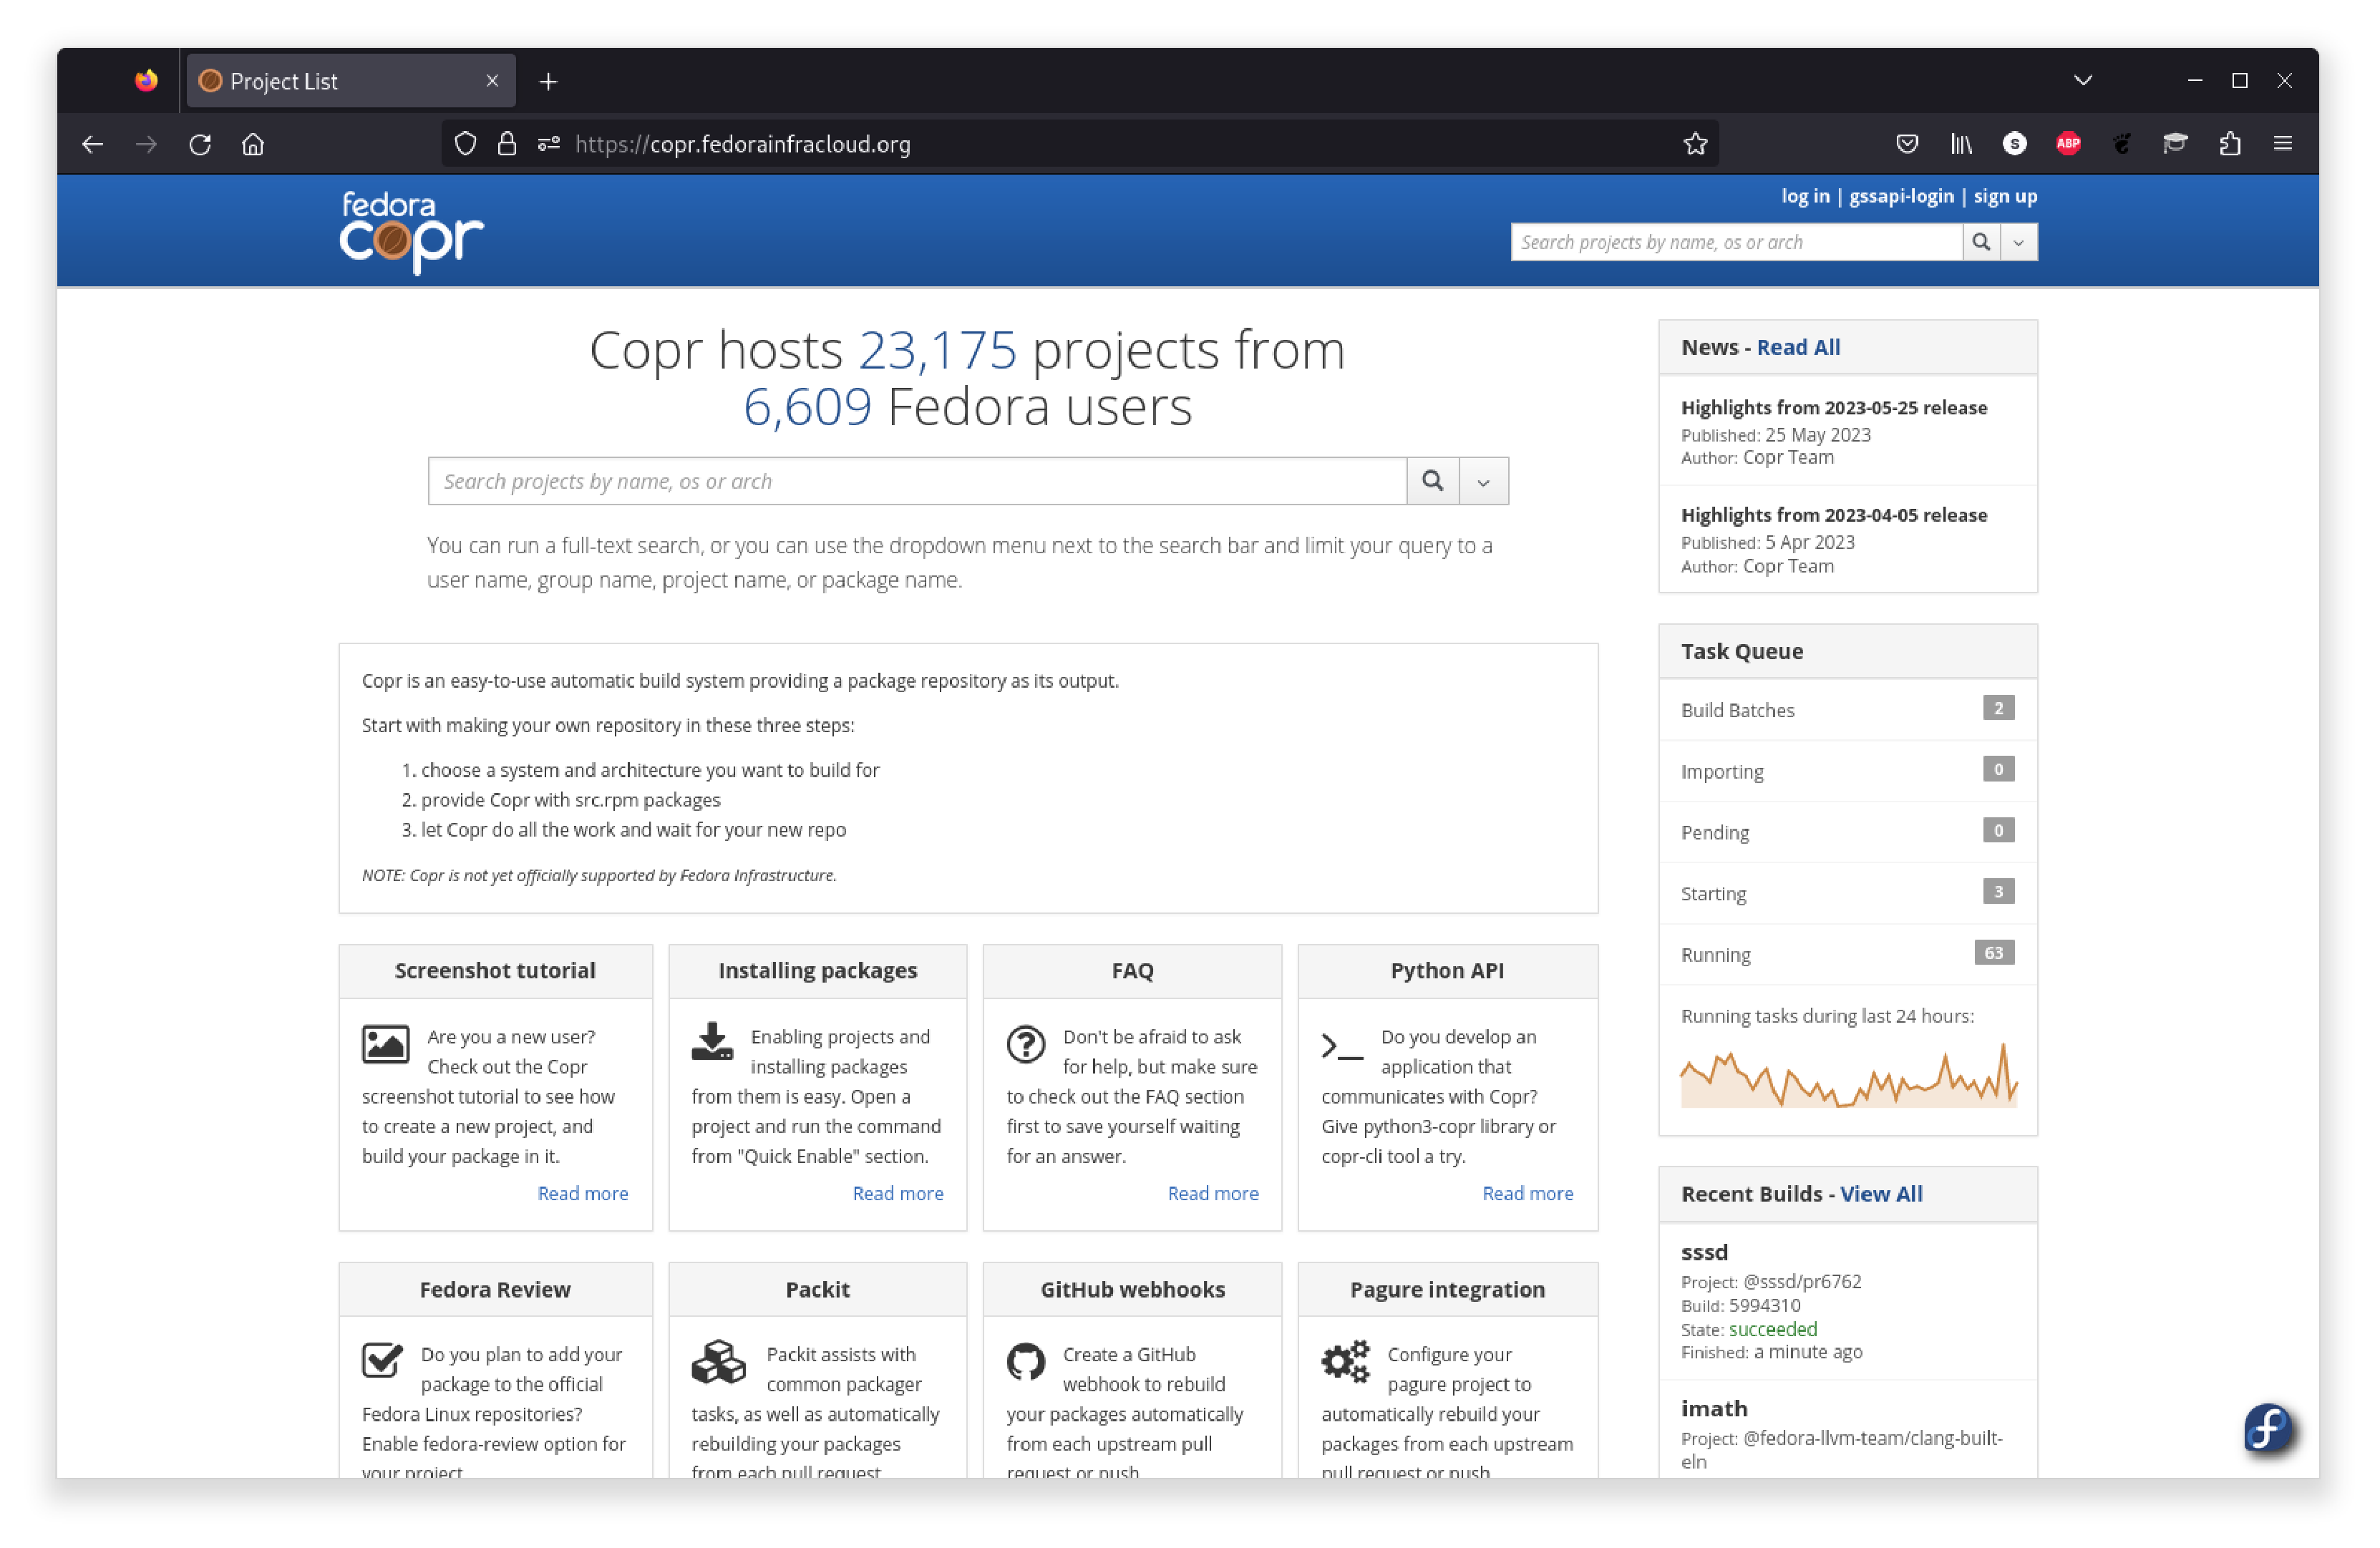
\includegraphics[width=1.0\textwidth,keepaspectratio=true,draft=\ddst]{img/rpms/copr.eps}
\end{center}
The Copr server is the closest thing to the official Fedora build system named \href{https://koji.fedoraproject.org/koji}{Koji}. \\
Also Copr has all the testing tools required to full-proof your RPM package before submitting it to Koji. \\[0.25cm]
The Copr user documentation is available at: \\[0.25cm]
\href{https://docs.pagure.org/copr.copr/user\_documentation.html}{https://docs.pagure.org/copr.copr/user\_documentation.html}
\newpage
\noindent Using Copr requires first of all to create a Fedora account at: \href{https://accounts.fedoraproject.org/}{https://accounts.fedoraproject.org/}
This Fedora account will be used for all Fedora resources, in particular Koji (see [Sec.~\ref{kojib}]). 
\begin{enumerate}
\item Register at \href{https://accounts.fedoraproject.org/}{https://accounts.fedoraproject.org/}
\begin{center}
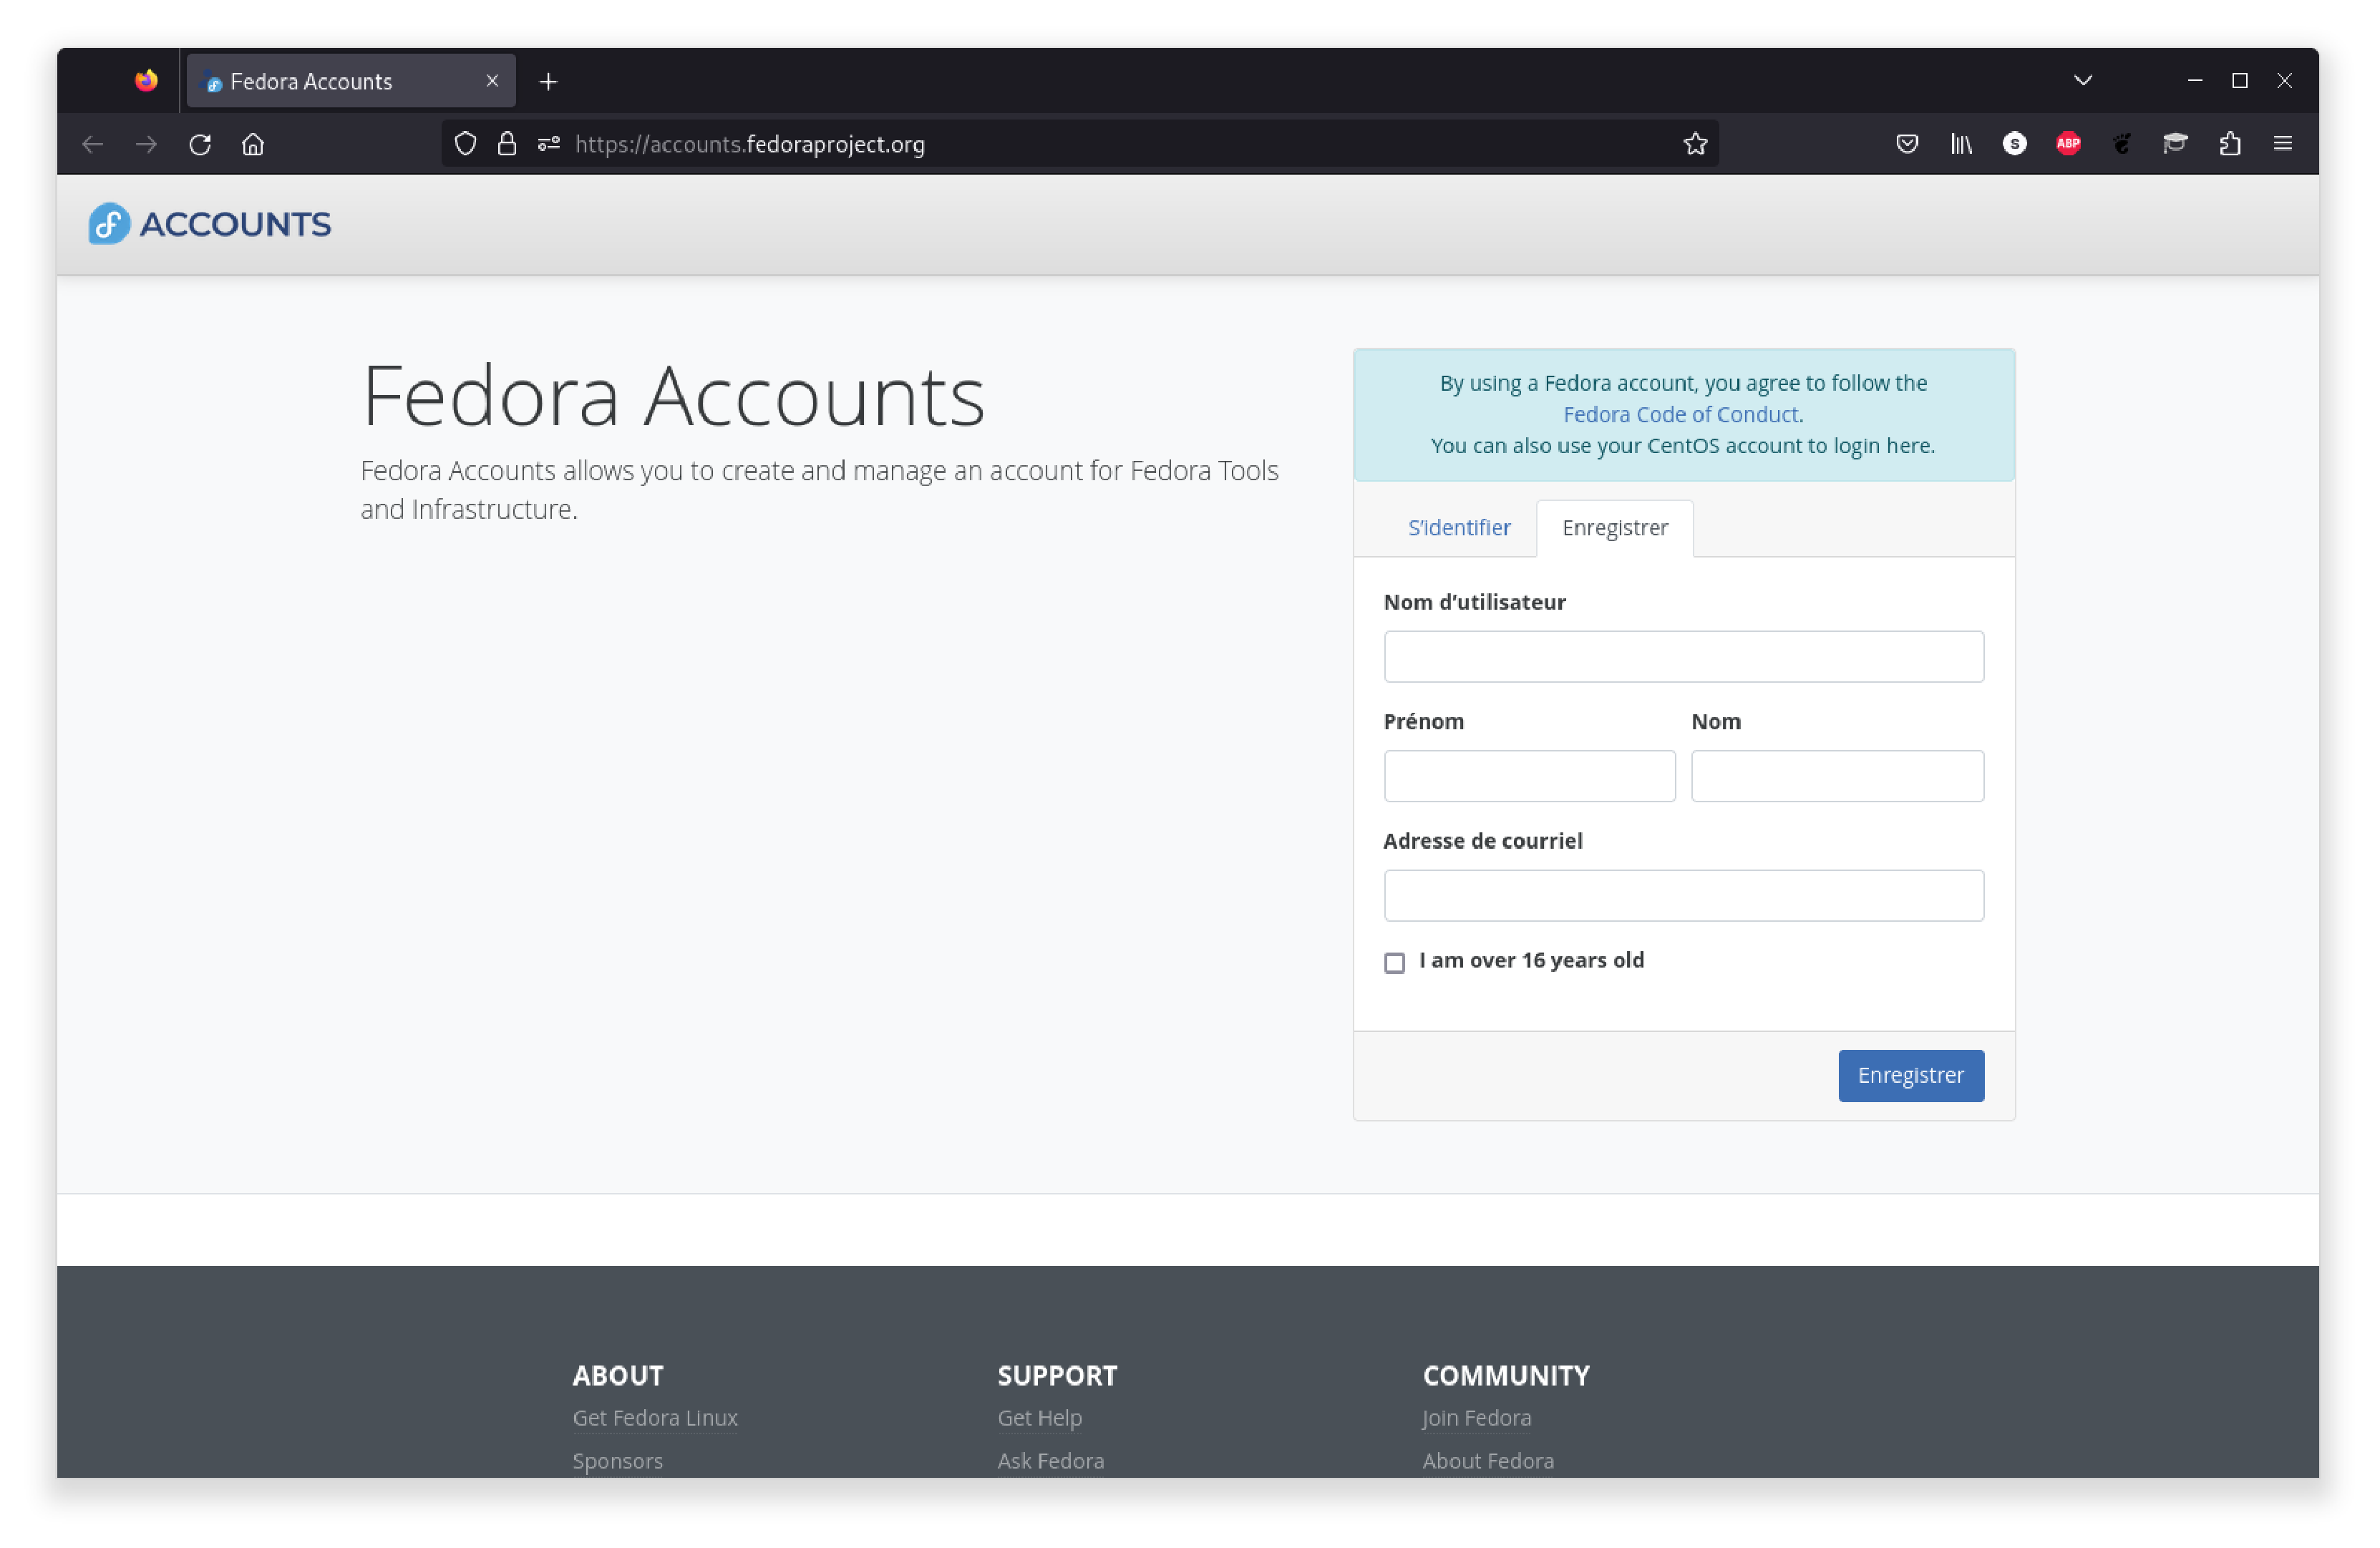
\includegraphics[width=0.7\textwidth,keepaspectratio=true,draft=\ddst]{img/rpms/f-account.eps}
\end{center}
\item After the registration sign the \href{https://docs.fedoraproject.org/en-US/legal/fpca/}{Fedora project Contributor Agreement}. 
\item Navigate to \href{https://copr.fedorainfracloud.org}{https://copr.fedorainfracloud.org} and login using your Fedora account. 
\begin{center}
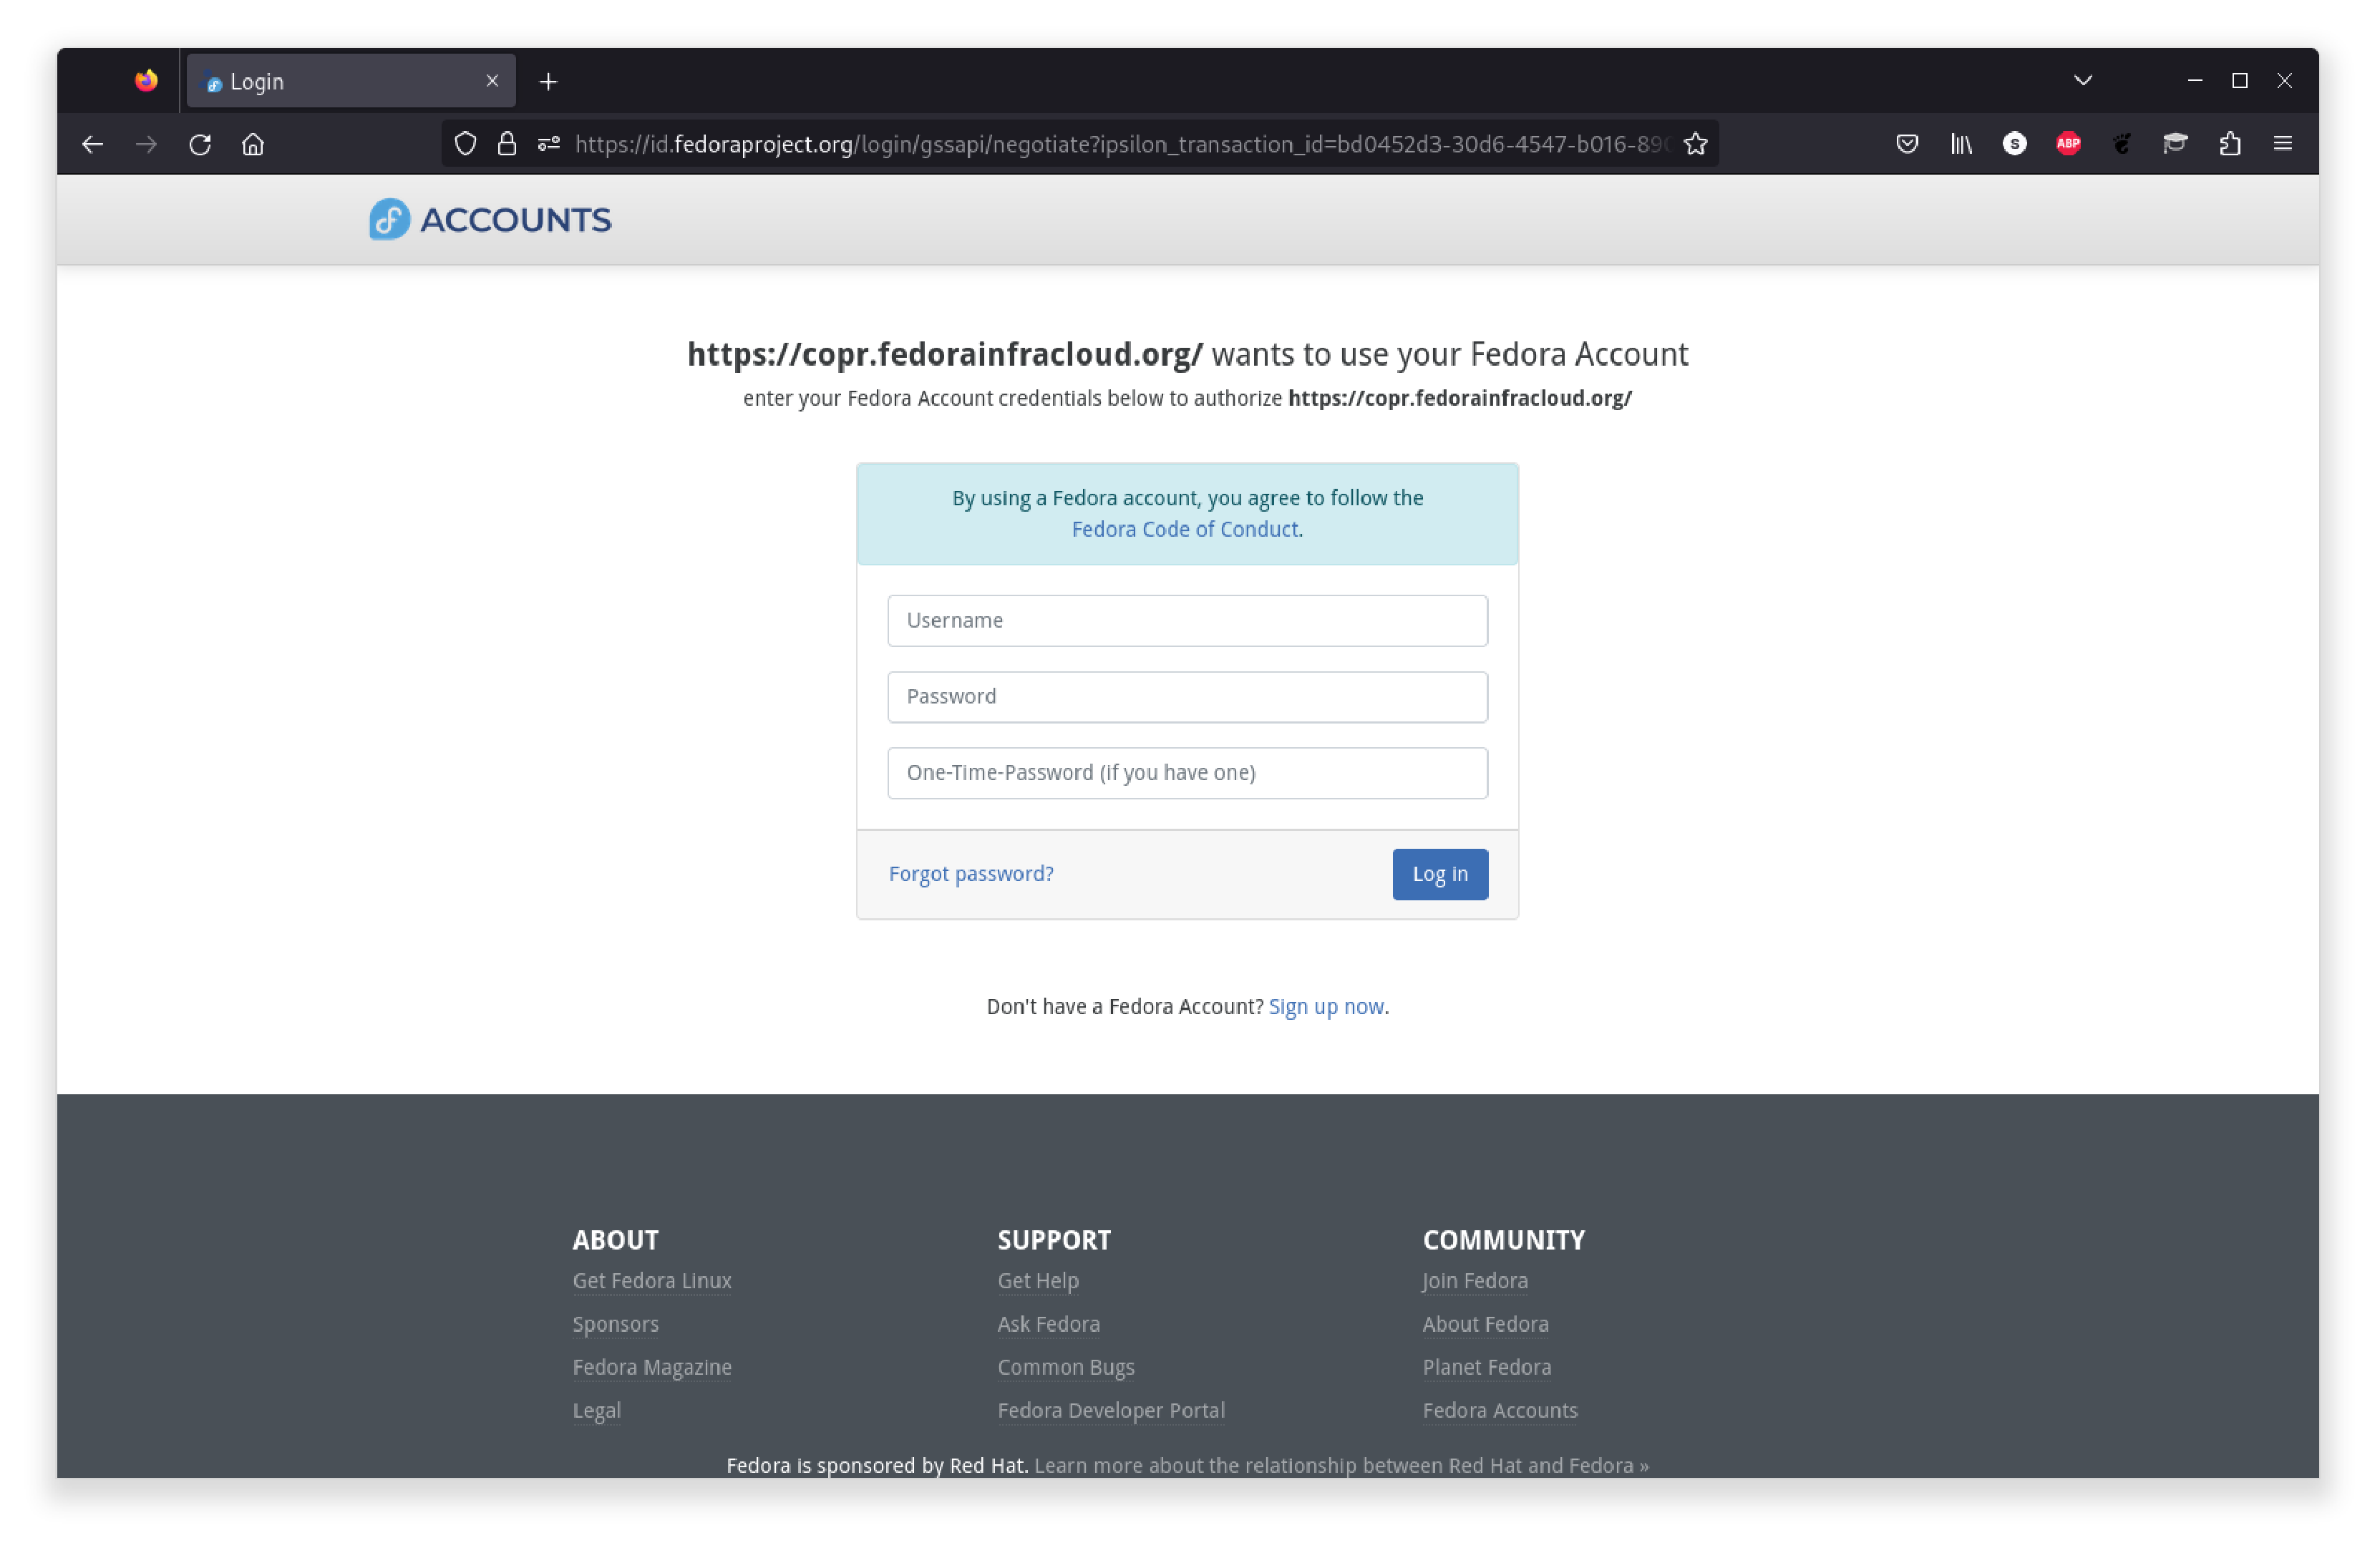
\includegraphics[width=0.7\textwidth,keepaspectratio=true,draft=\ddst]{img/rpms/c-login.eps}
\end{center}
Remember, and store, the Fedora username and password that you created at this stage since they will be used on regular basis if you integrate the Fedora network and building tools (Koji, see [Sec.~\ref{kojib}]). 
\newpage
\item Create a new project to host your work in Copr: 
\begin{itemize}
\item Describe the project (you can use Markdown):
\begin{center}
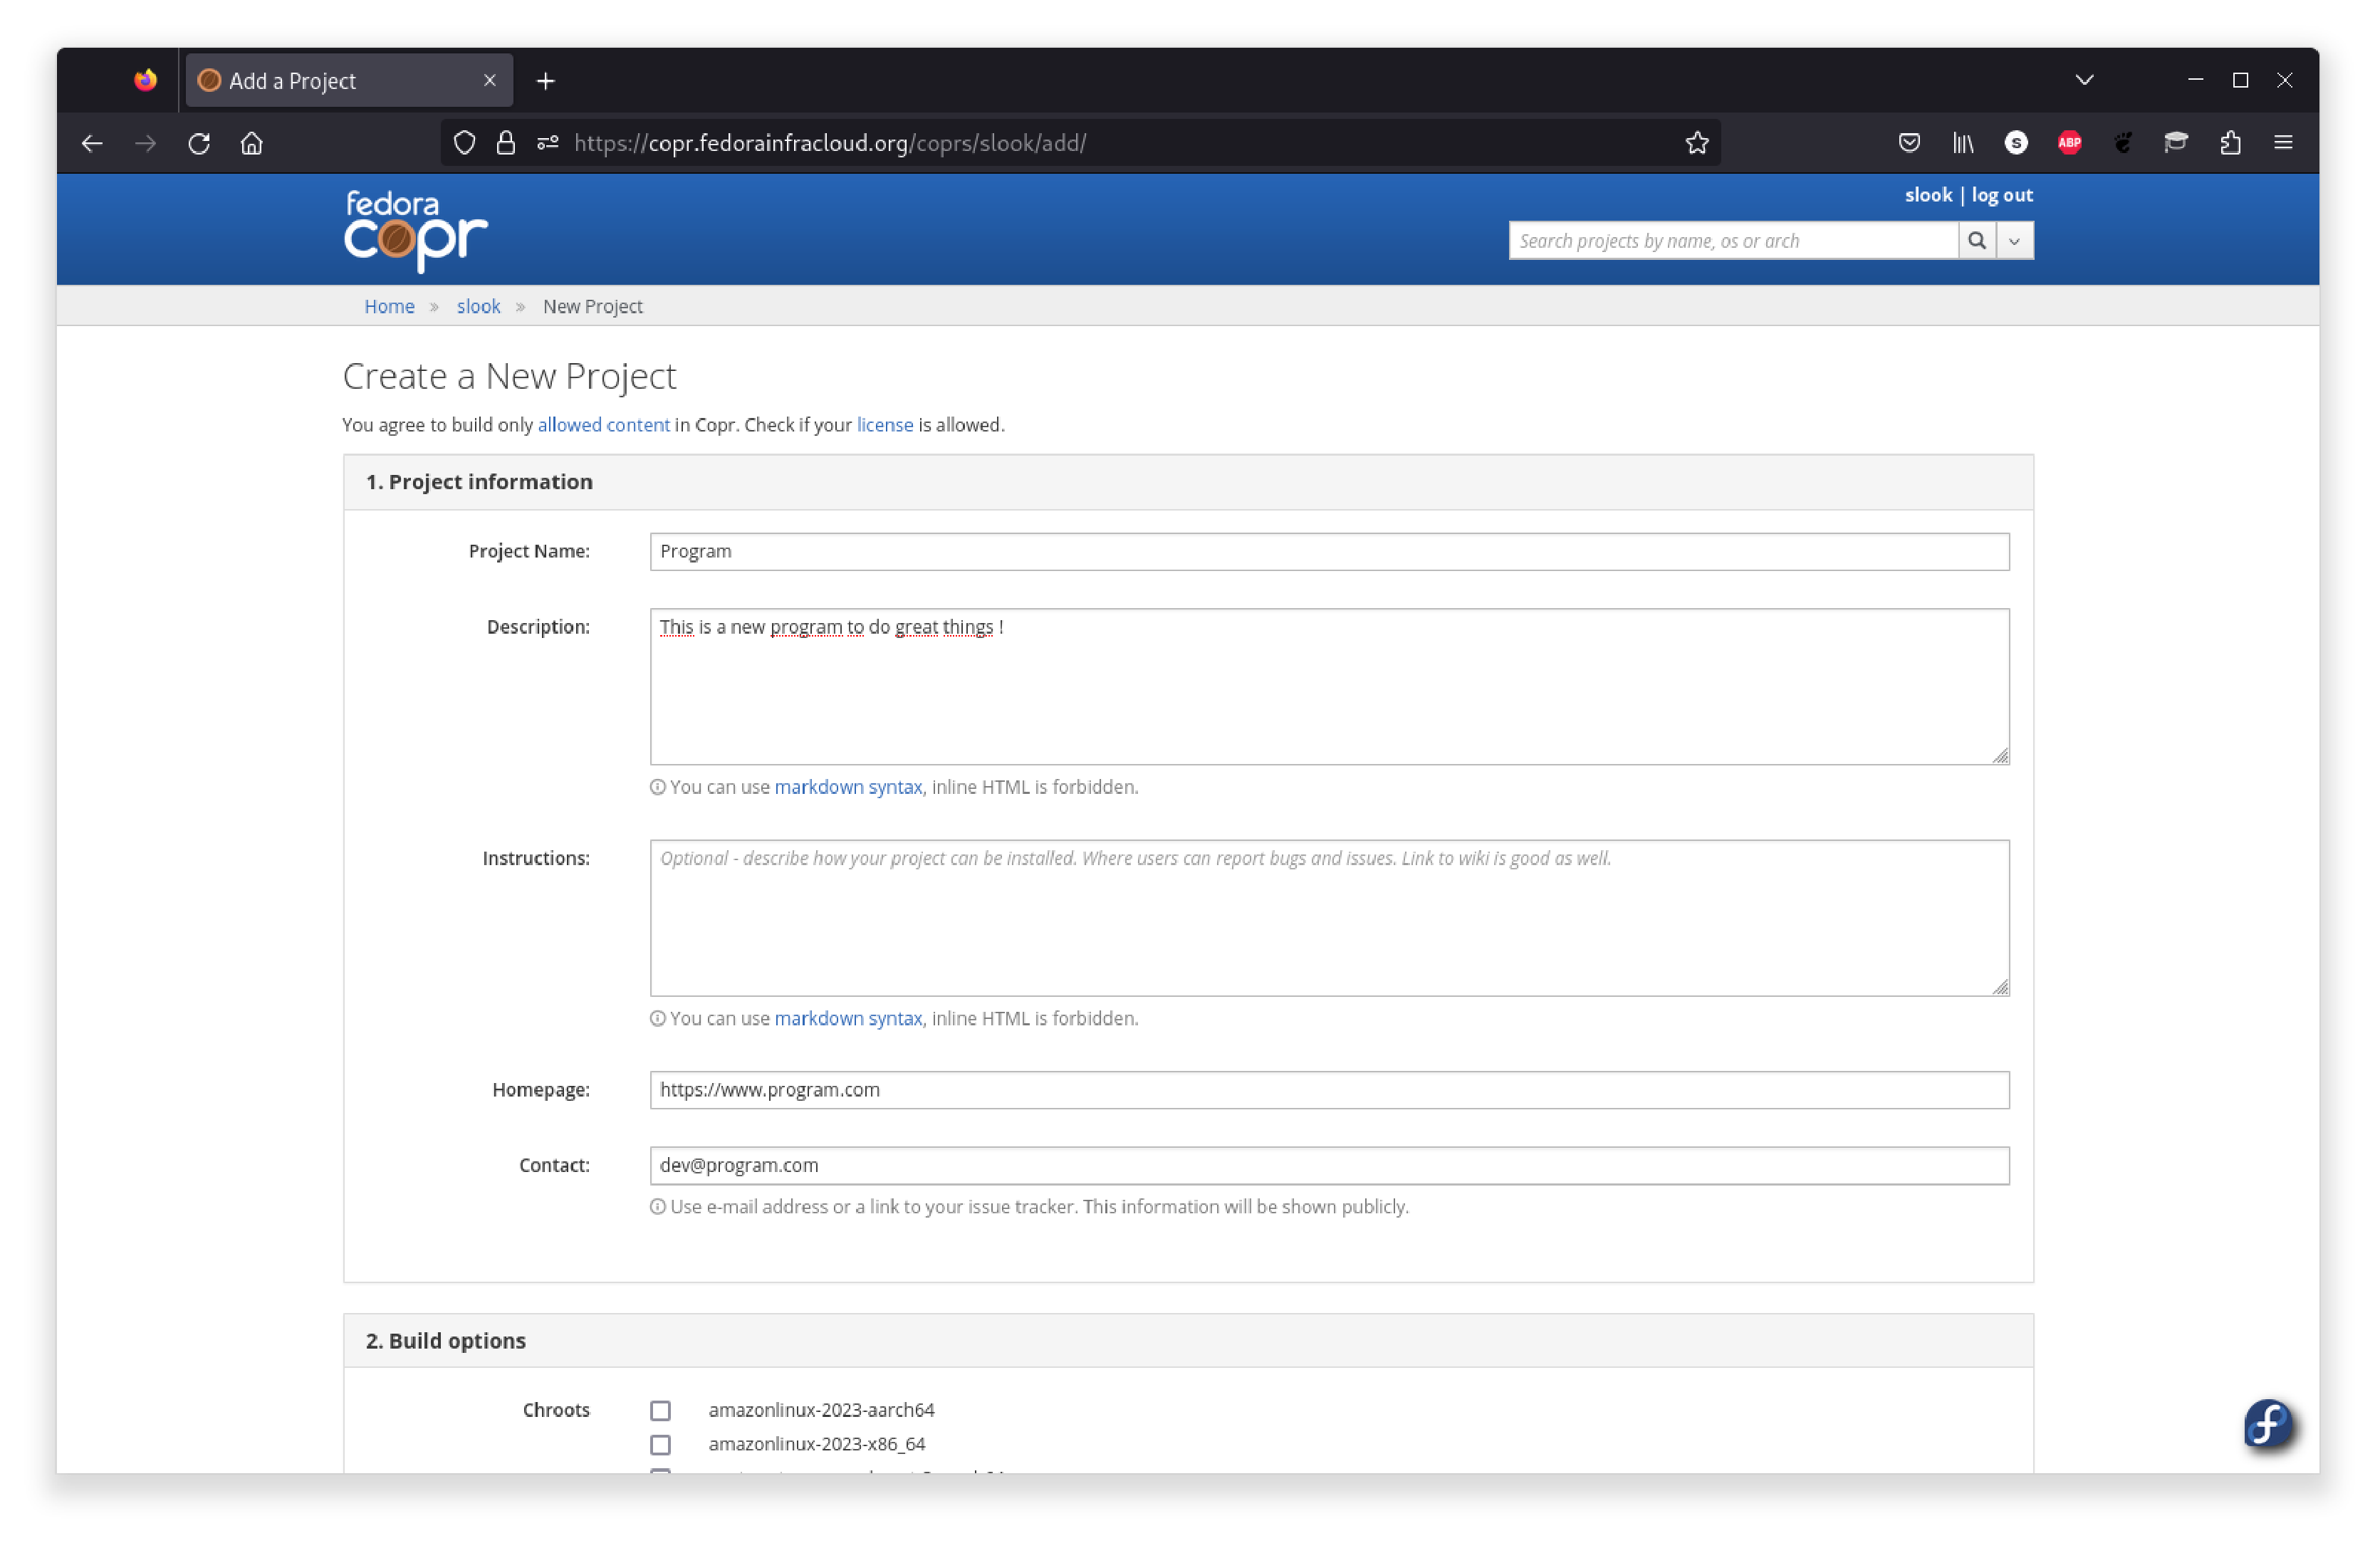
\includegraphics[width=0.6\textwidth,keepaspectratio=true,draft=\ddst]{img/rpms/new-p-1.eps}
\end{center}
\item Select the target architecture(s):
\begin{center}
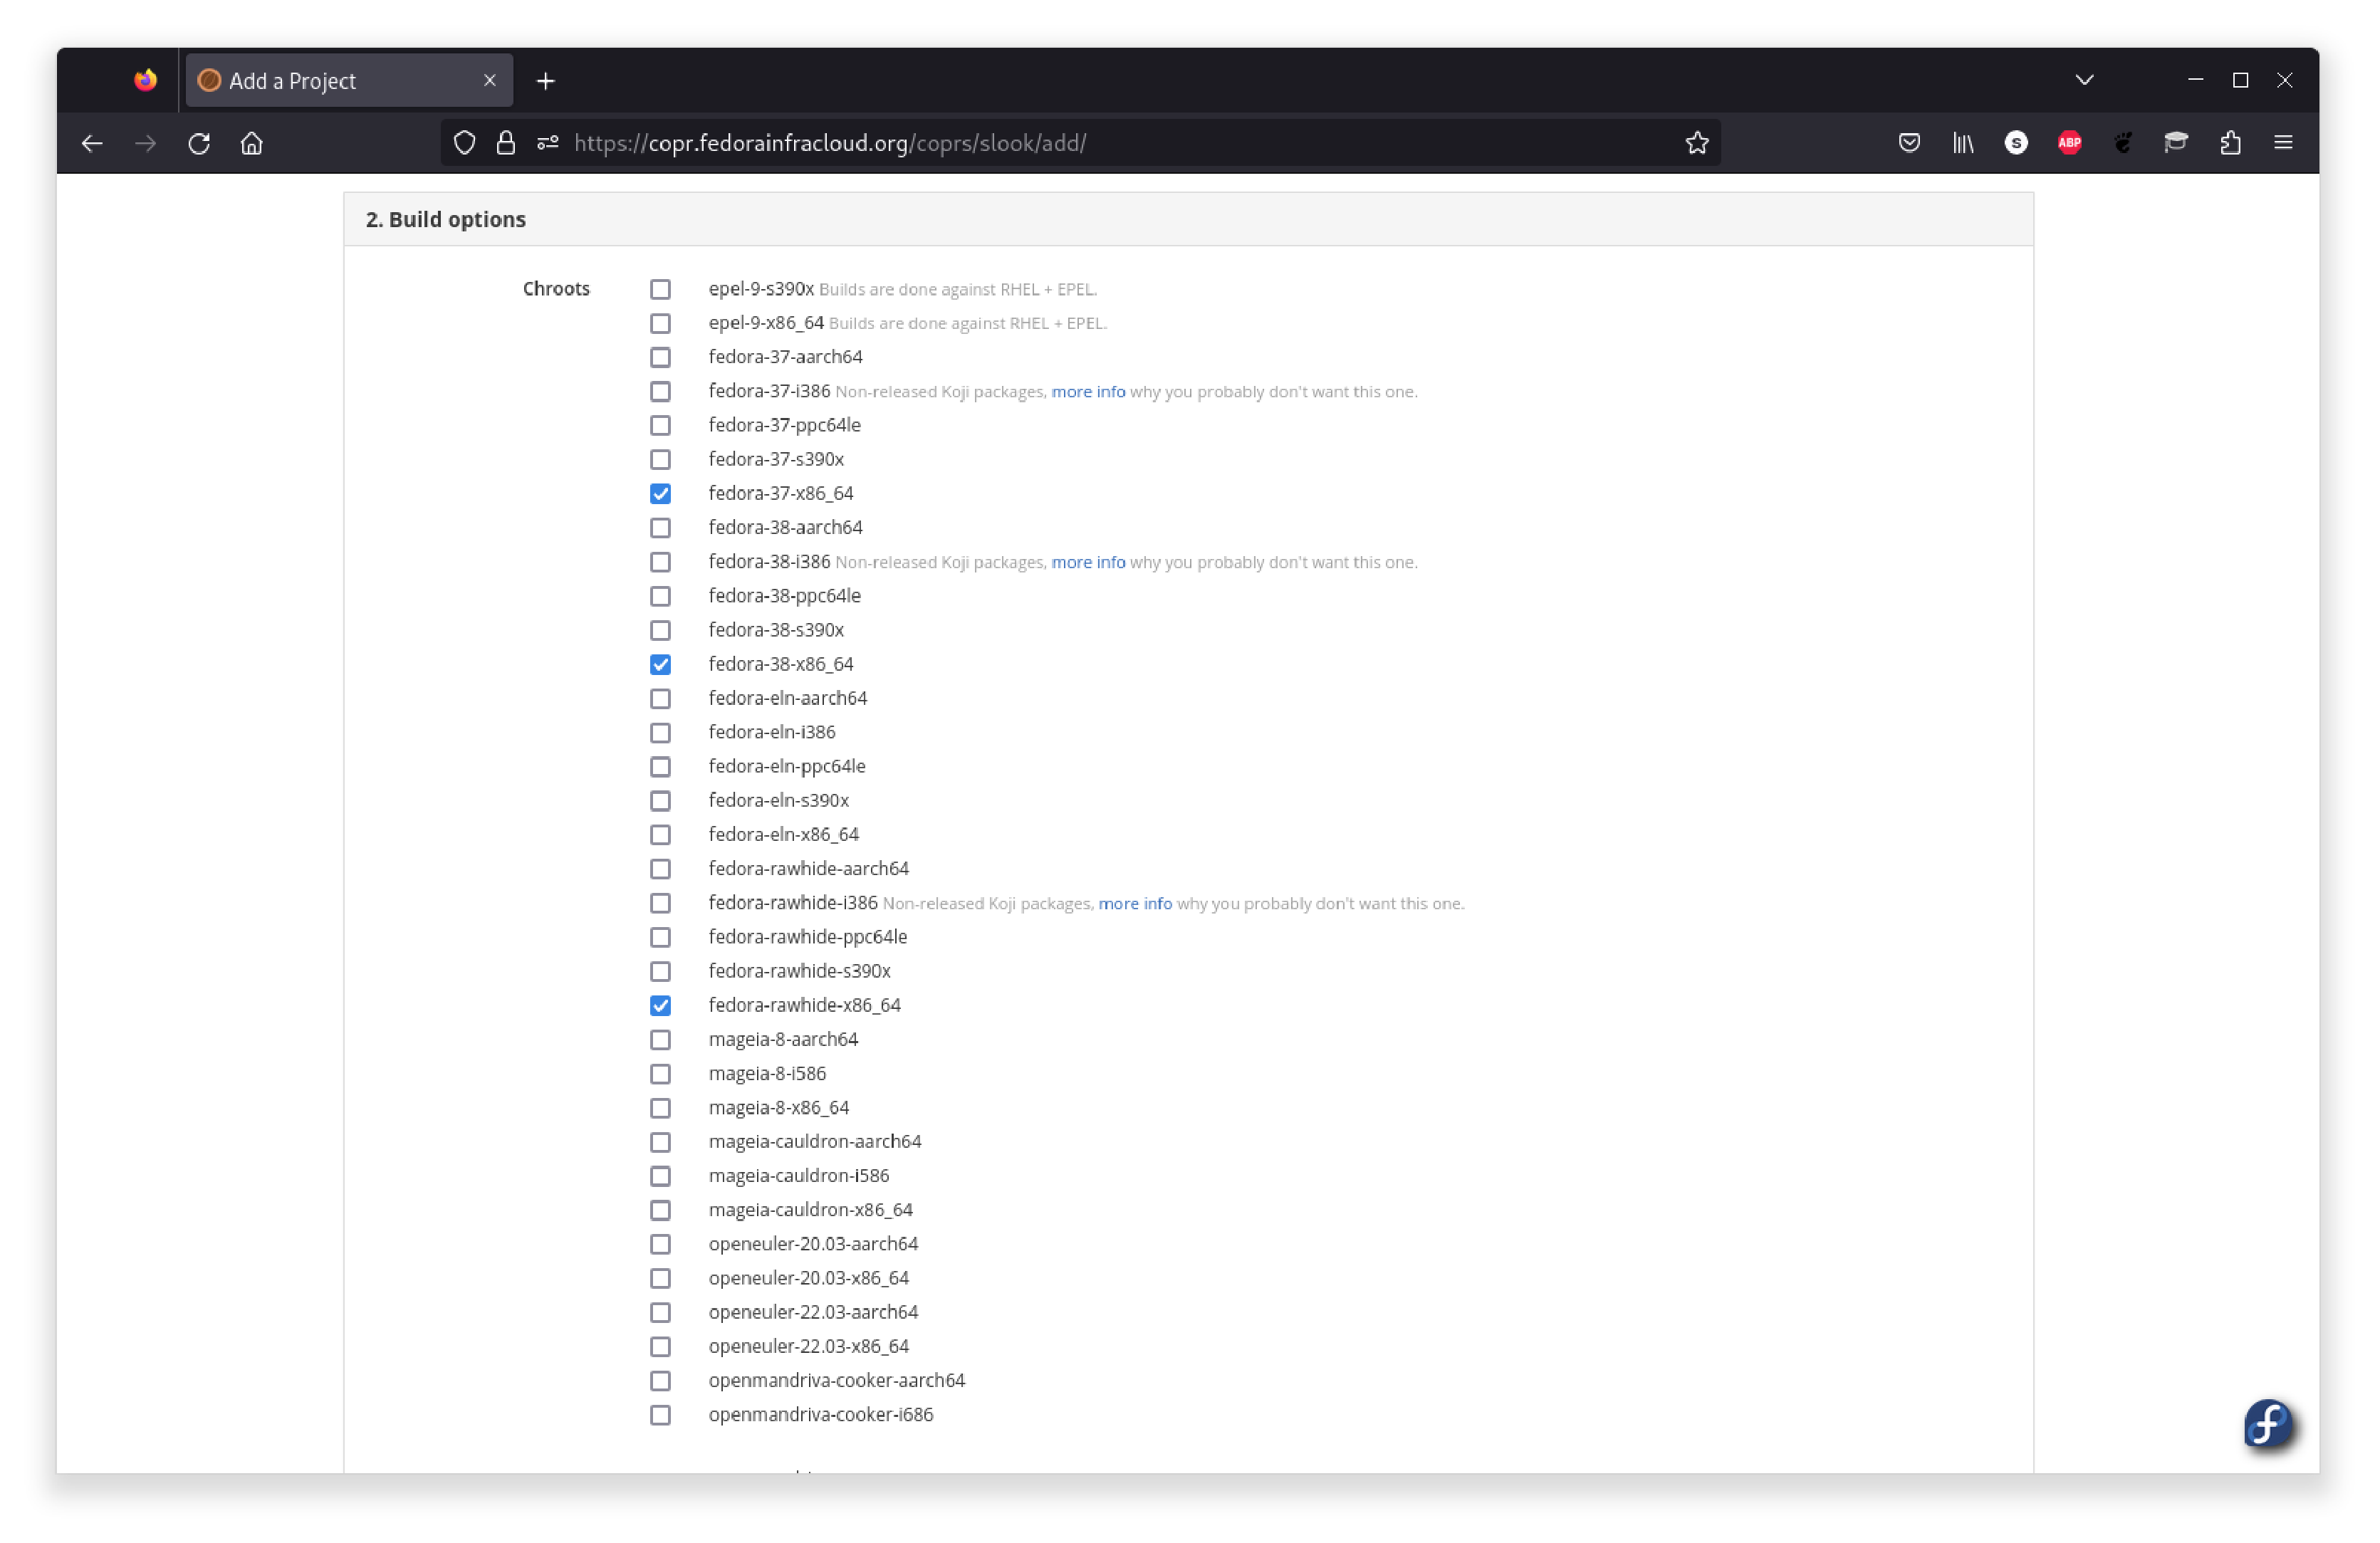
\includegraphics[width=0.6\textwidth,keepaspectratio=true,draft=\ddst]{img/rpms/new-p-2.eps}
\end{center}
\item Scroll down and click on "Create":
\begin{center}
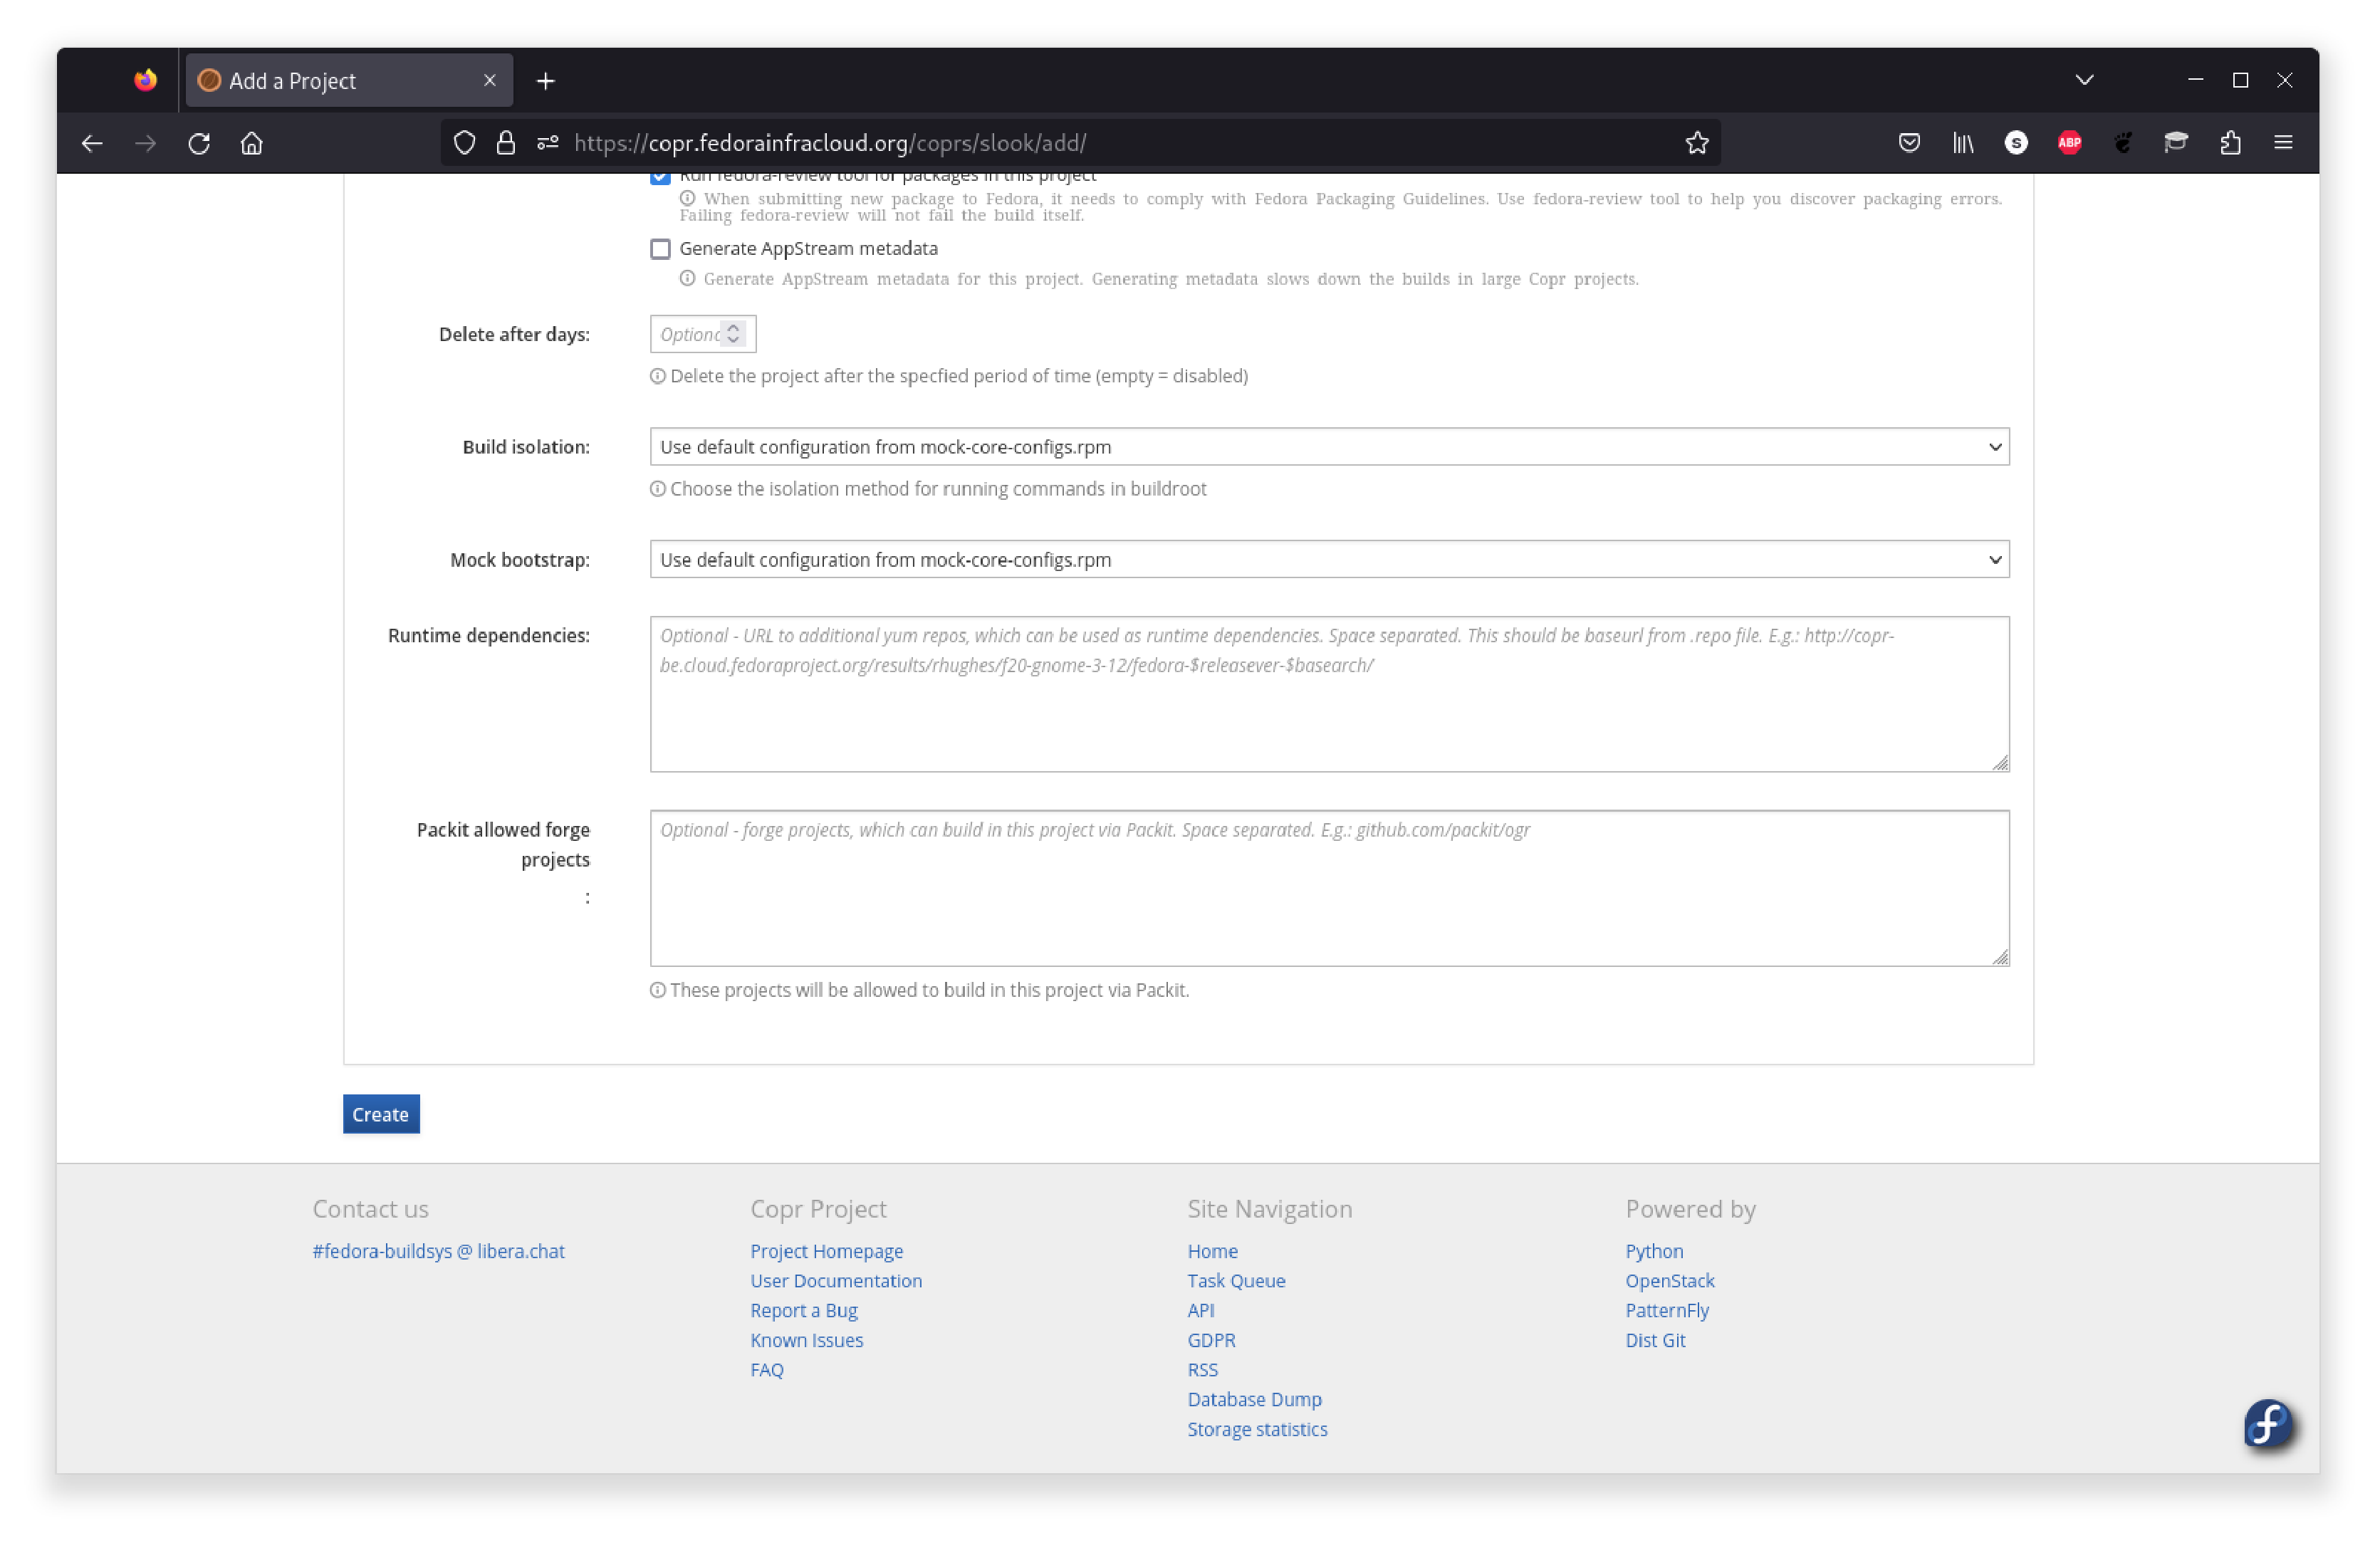
\includegraphics[width=0.6\textwidth,keepaspectratio=true,draft=\ddst]{img/rpms/new-p-3.eps}
\end{center}
\end{itemize}
\newpage
\item Then "Submit a New Build" for the project:
\begin{center}
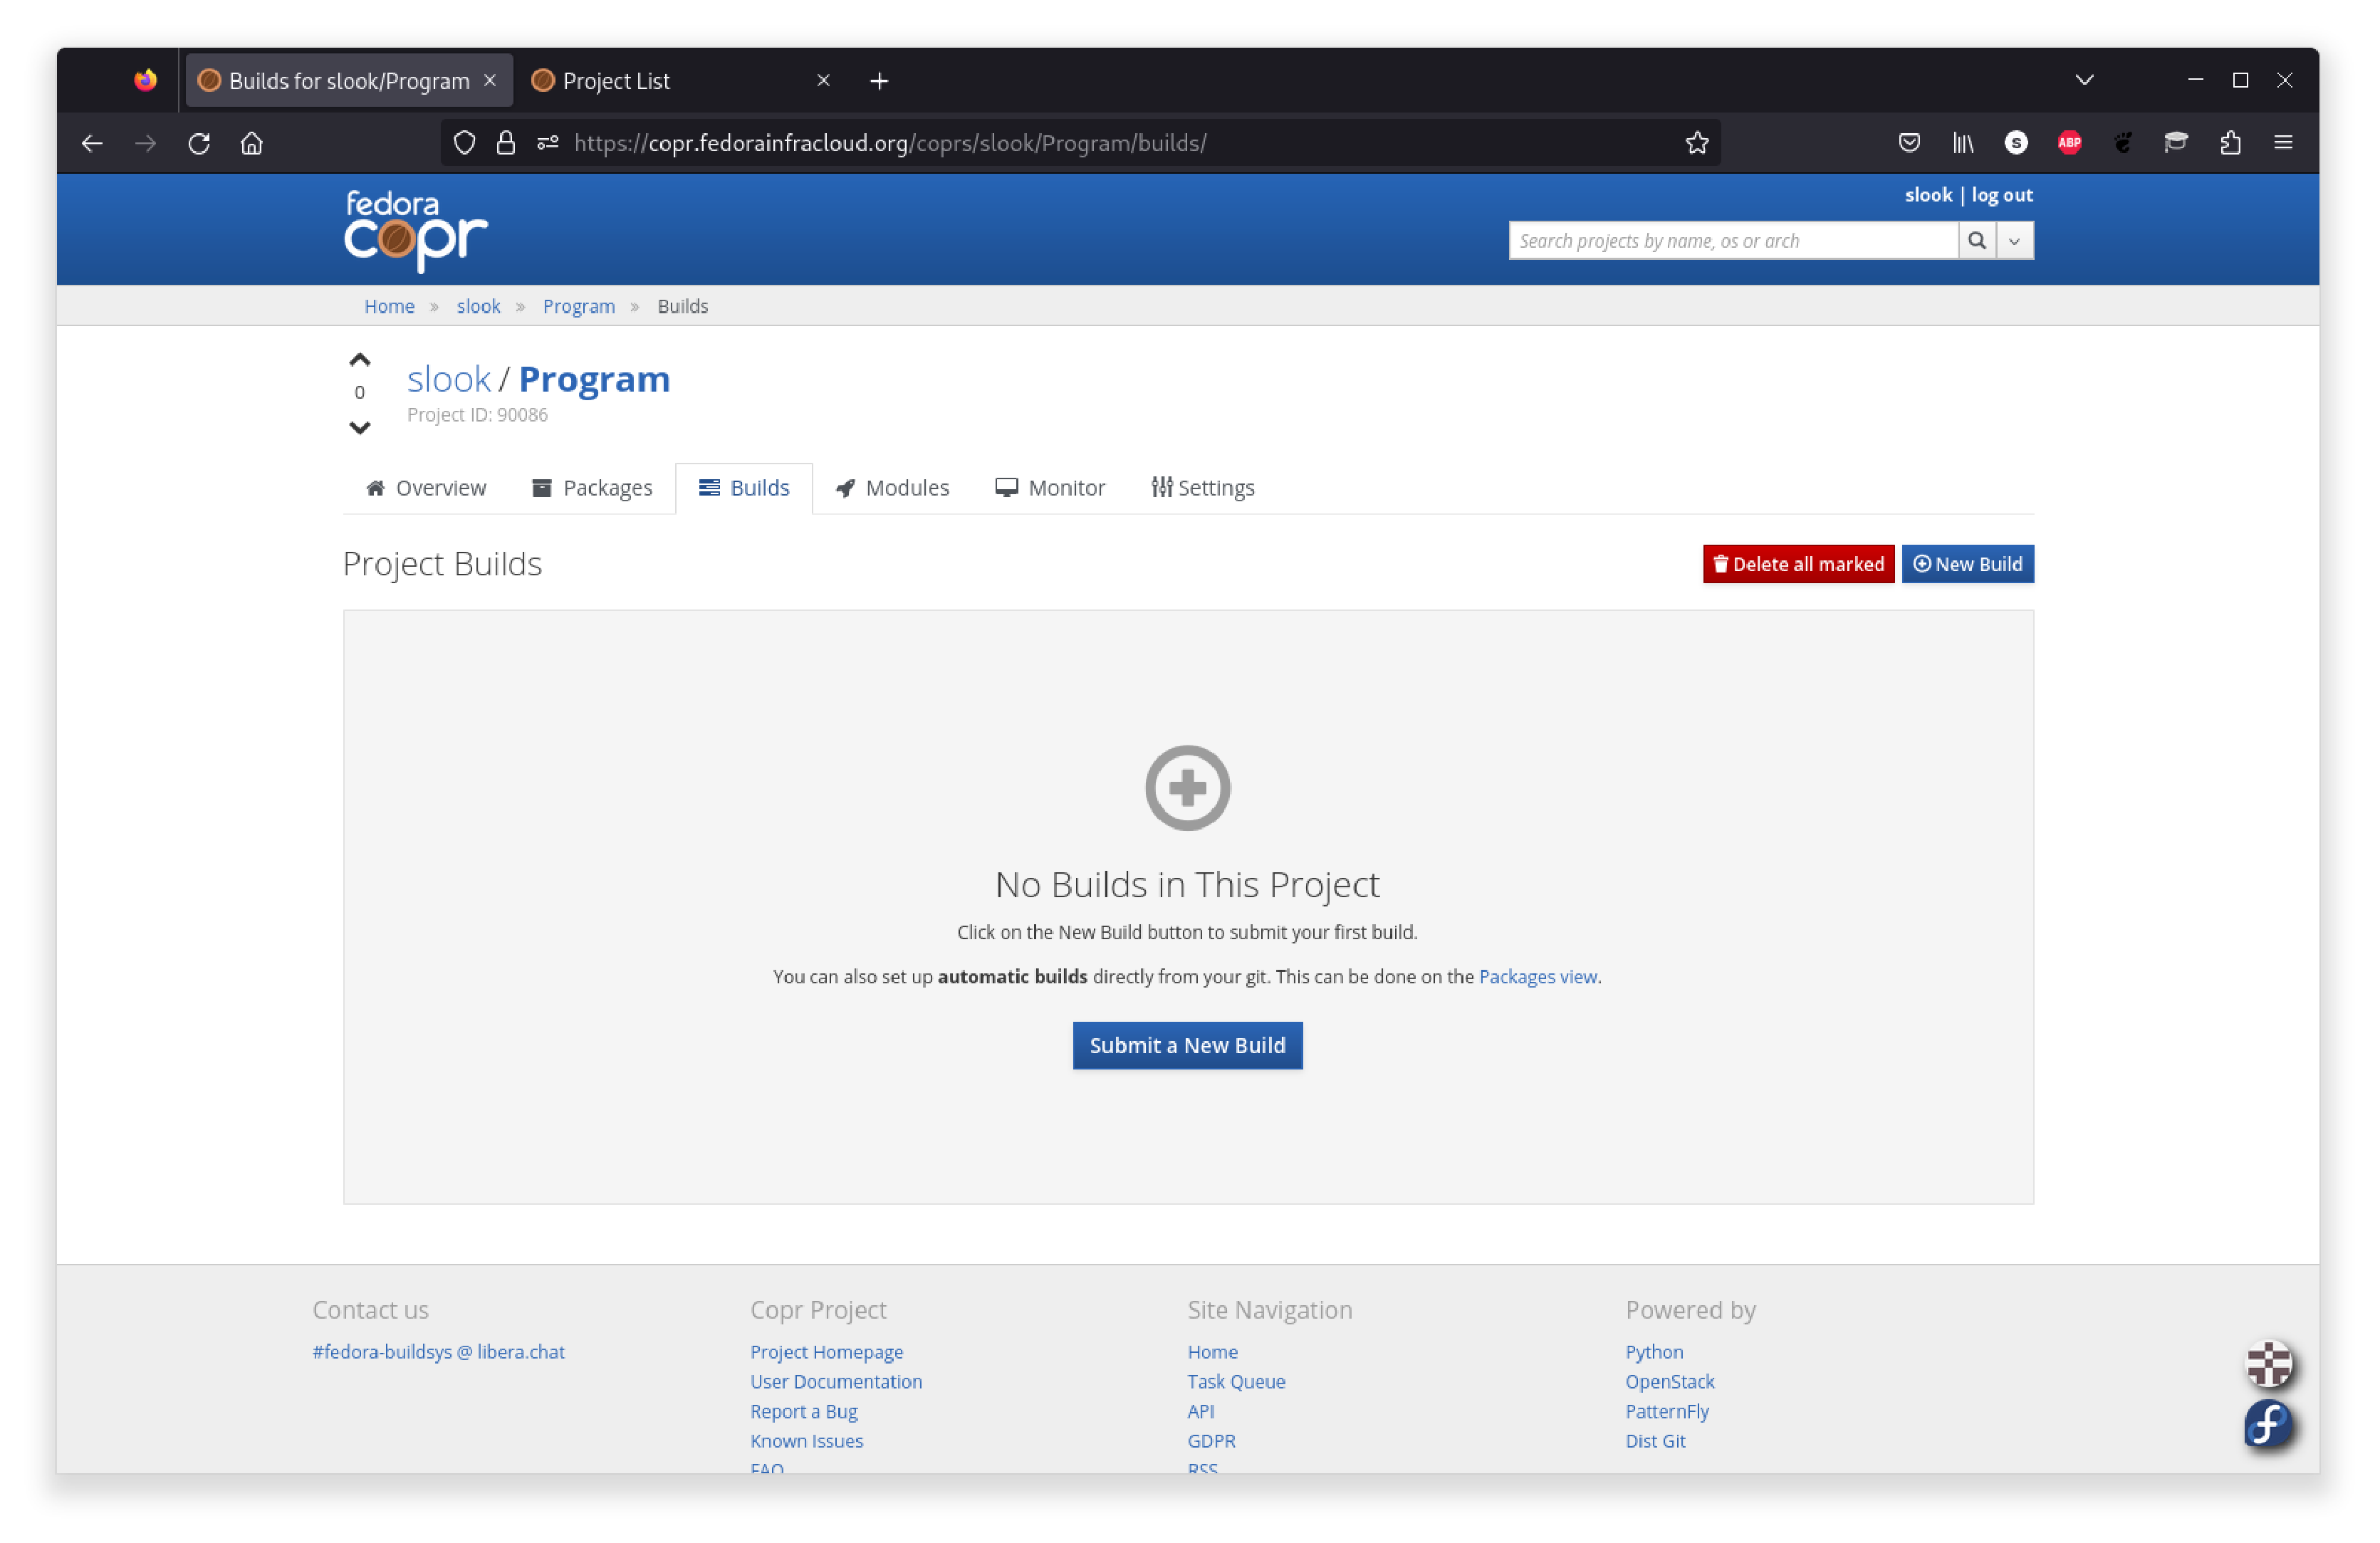
\includegraphics[width=0.6\textwidth,keepaspectratio=true,draft=\ddst]{img/rpms/build-1.eps}
\end{center}
\item Build the project:
\begin{itemize}
\item Build from URL, and specify the URL of your "\bftt{.spec}" file:
\begin{center}
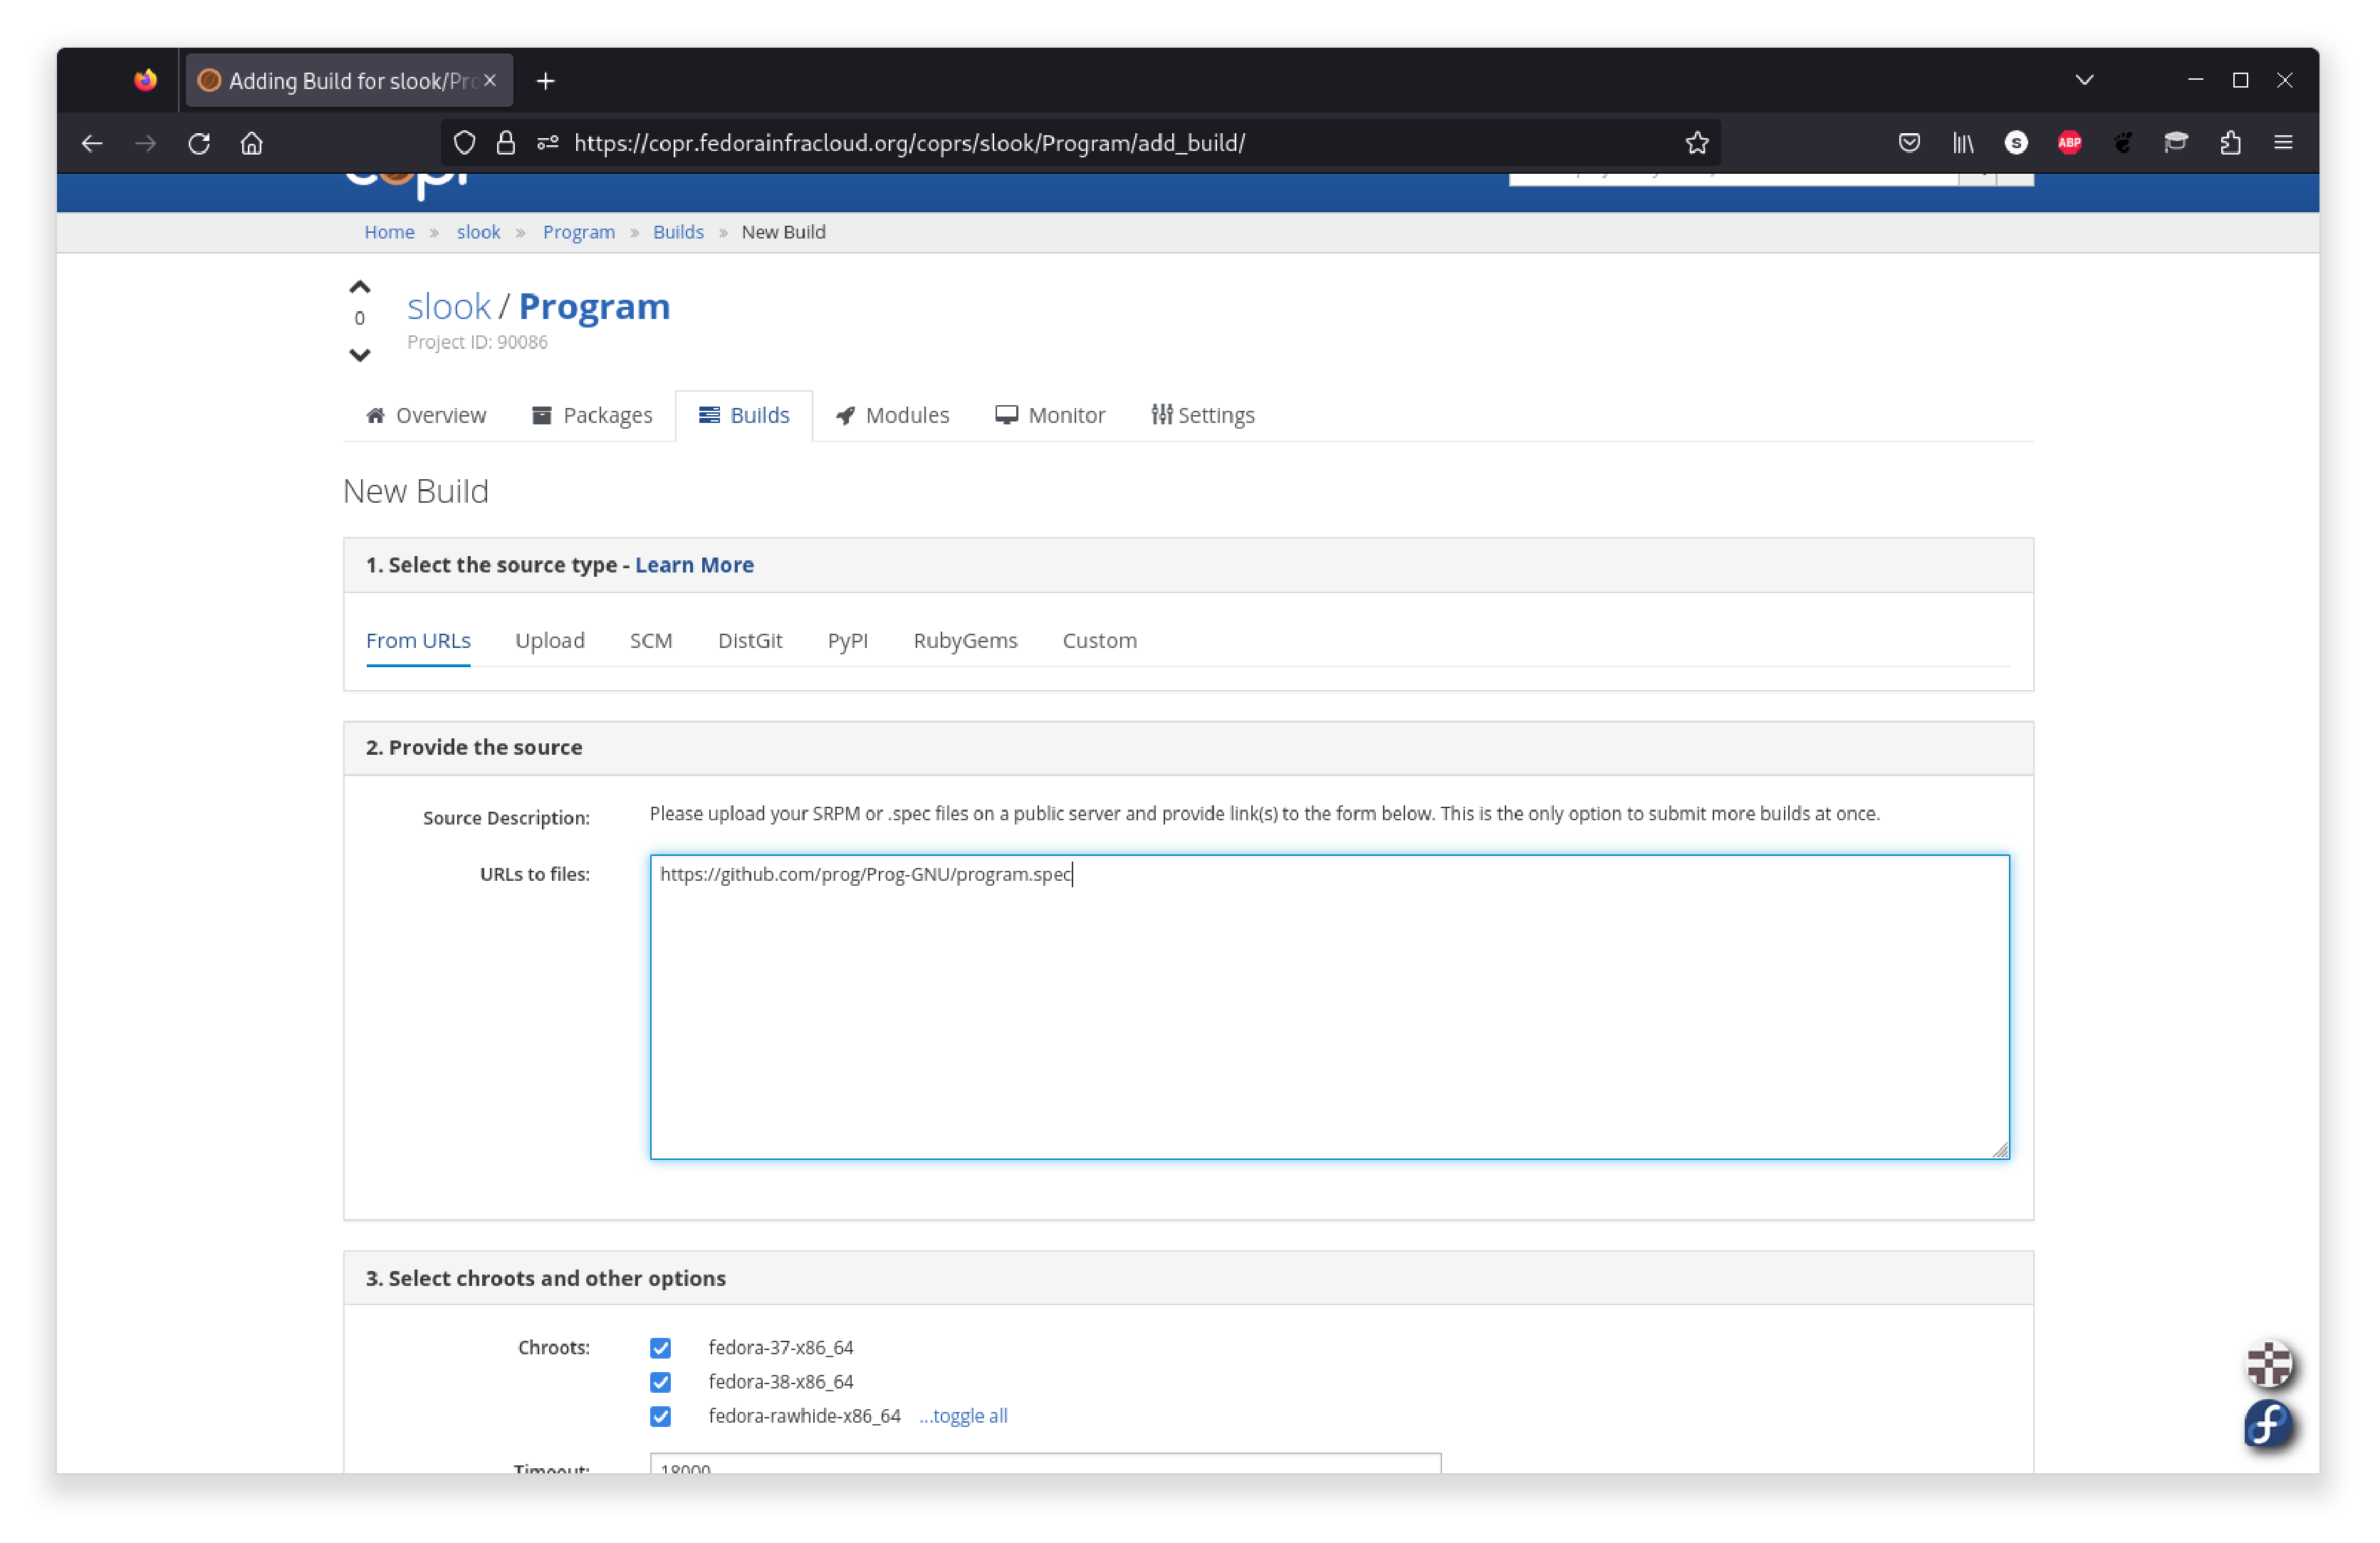
\includegraphics[width=0.6\textwidth,keepaspectratio=true,draft=\ddst]{img/rpms/build-2.eps}
\end{center}
\item Scroll down and simply click on "Build":
\begin{center}
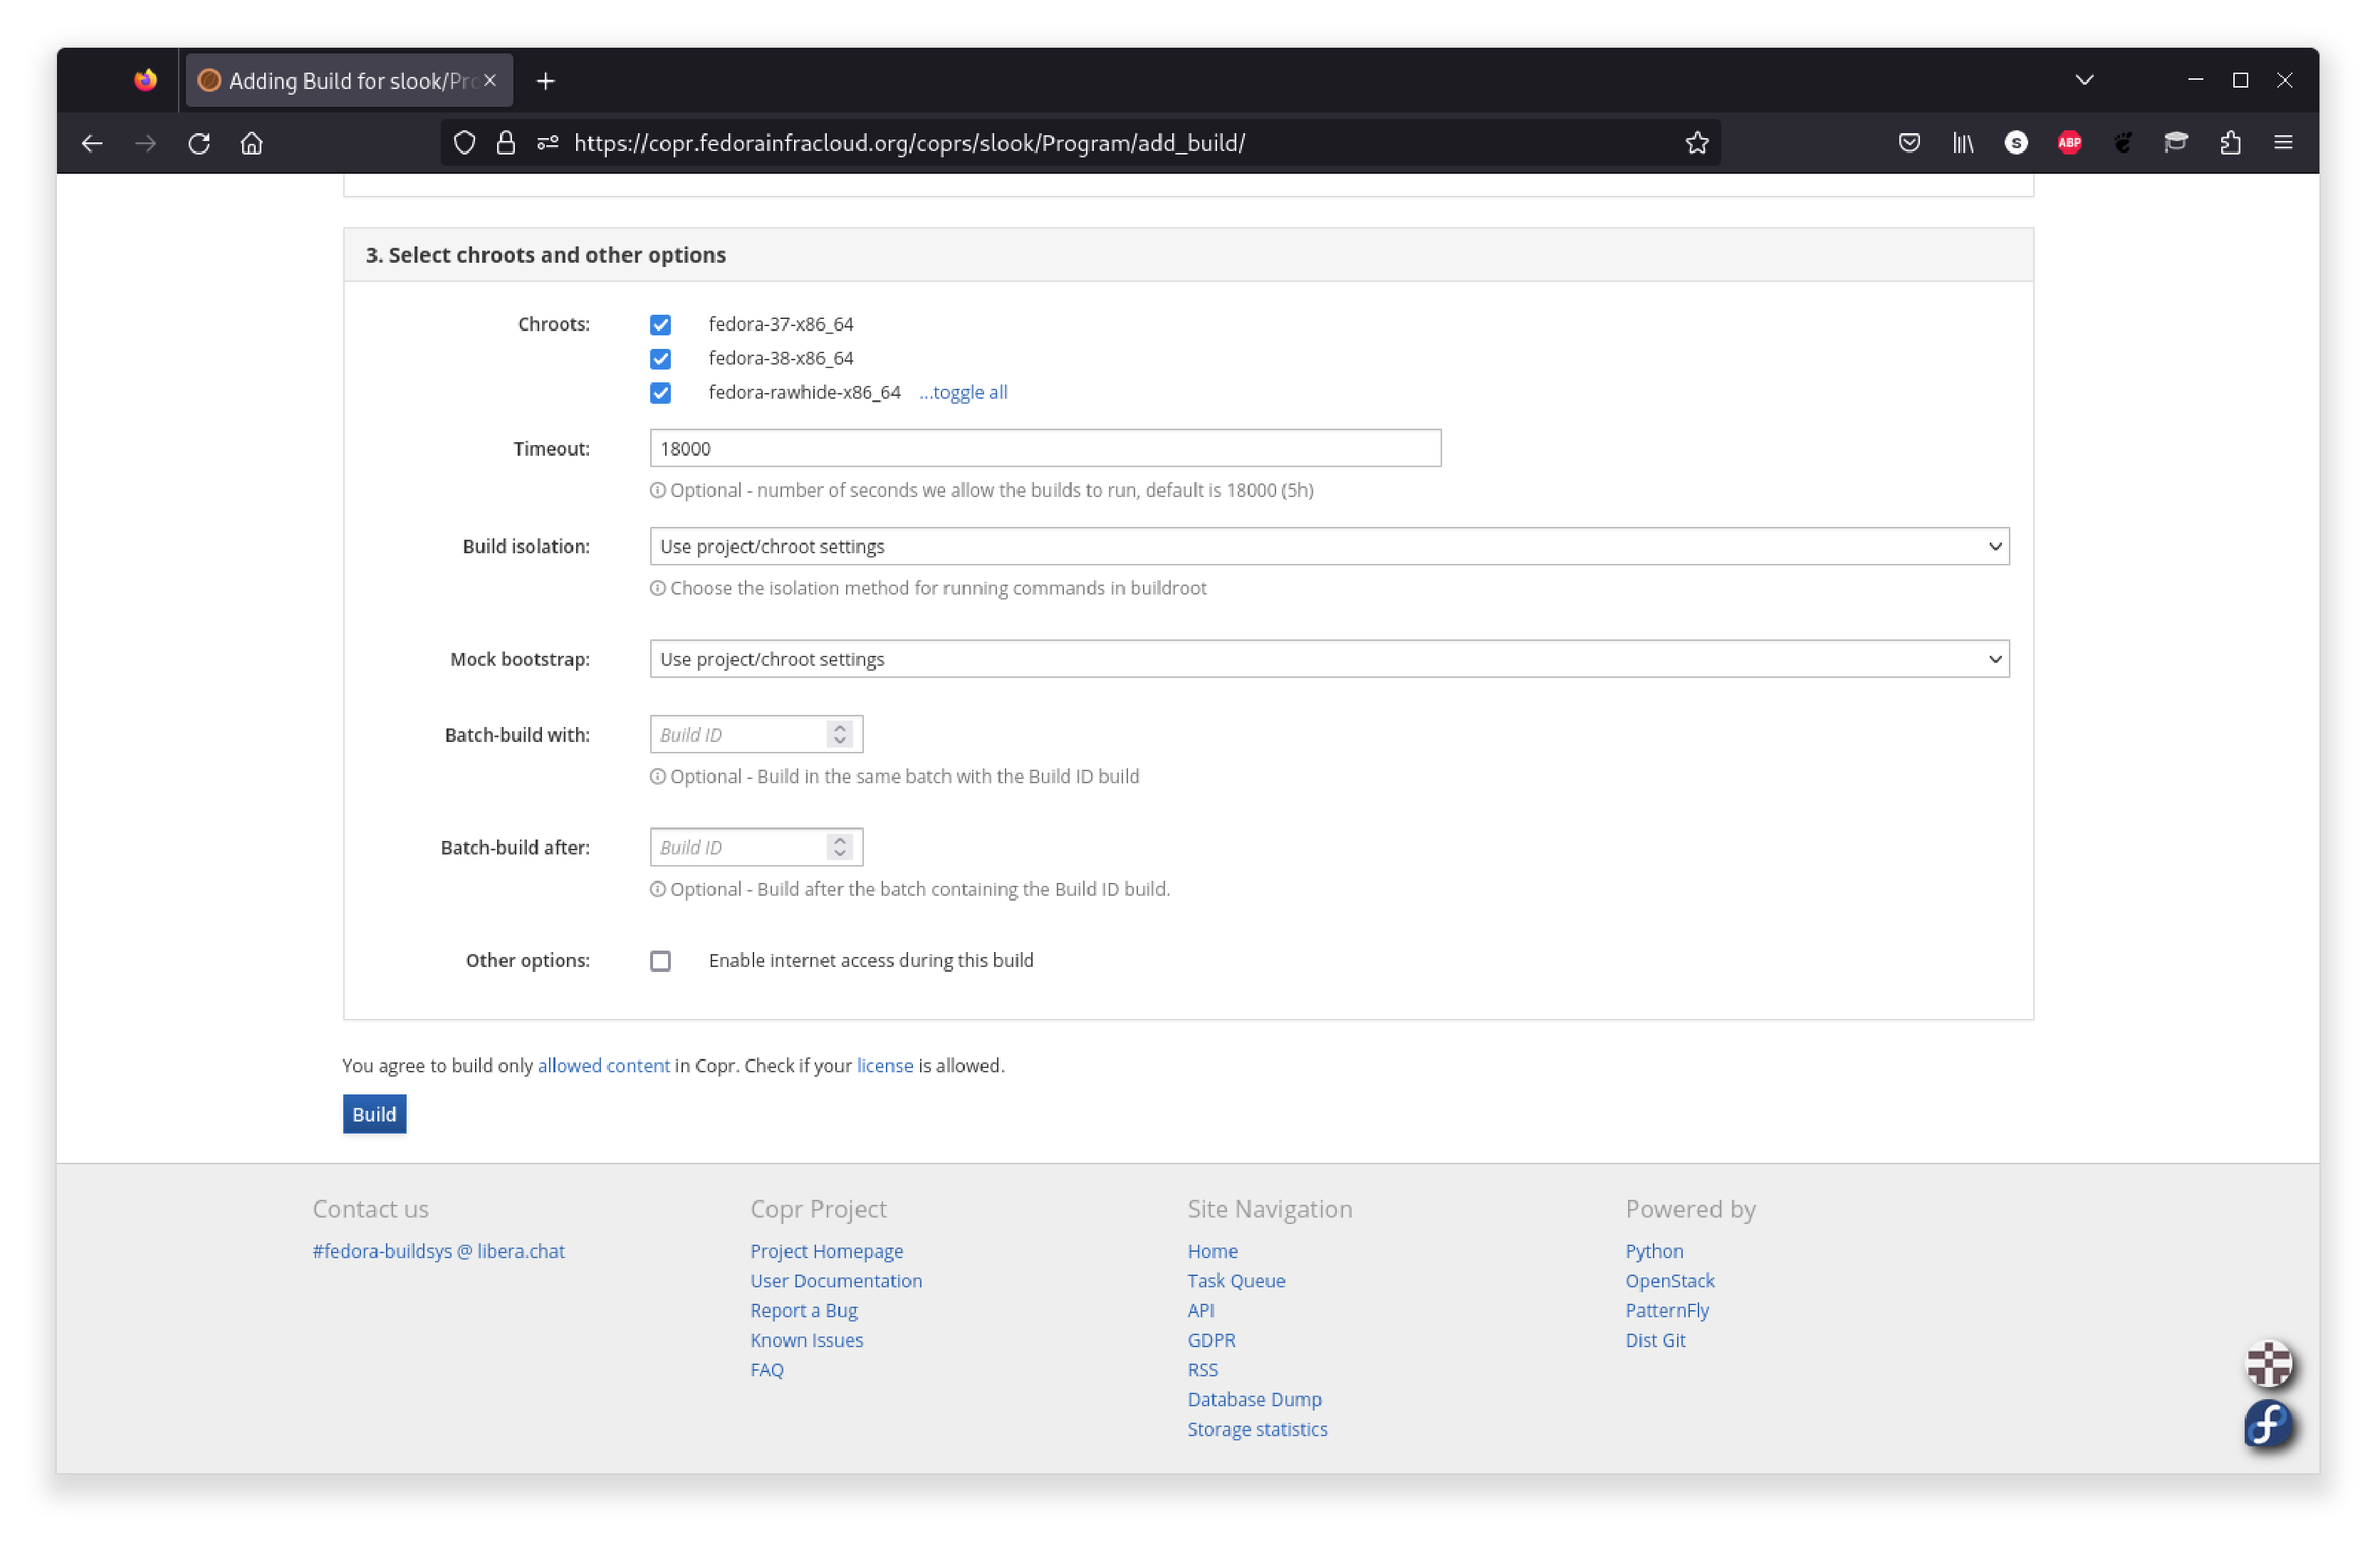
\includegraphics[width=0.6\textwidth,keepaspectratio=true,draft=\ddst]{img/rpms/build-3.eps}
\end{center}
\end{itemize}
\end{enumerate}
At this point Copr is going to use the specified "\bftt{.spec}" file to build the RPMs of your project. \\
Providing that the "\bftt{.spec}" file properly describes the sources location and the actions needed to build the RPM, 
then nothing else is required. 

\subsubsection{Koji build}
\label{kojib}

\href{https://fedoraproject.org/wiki/Koji}{Koji} is the official RPM build system of the Fedora project: \href{https://koji.fedoraproject.org/koji}{https://koji.fedoraproject.org/koji}
\begin{center}
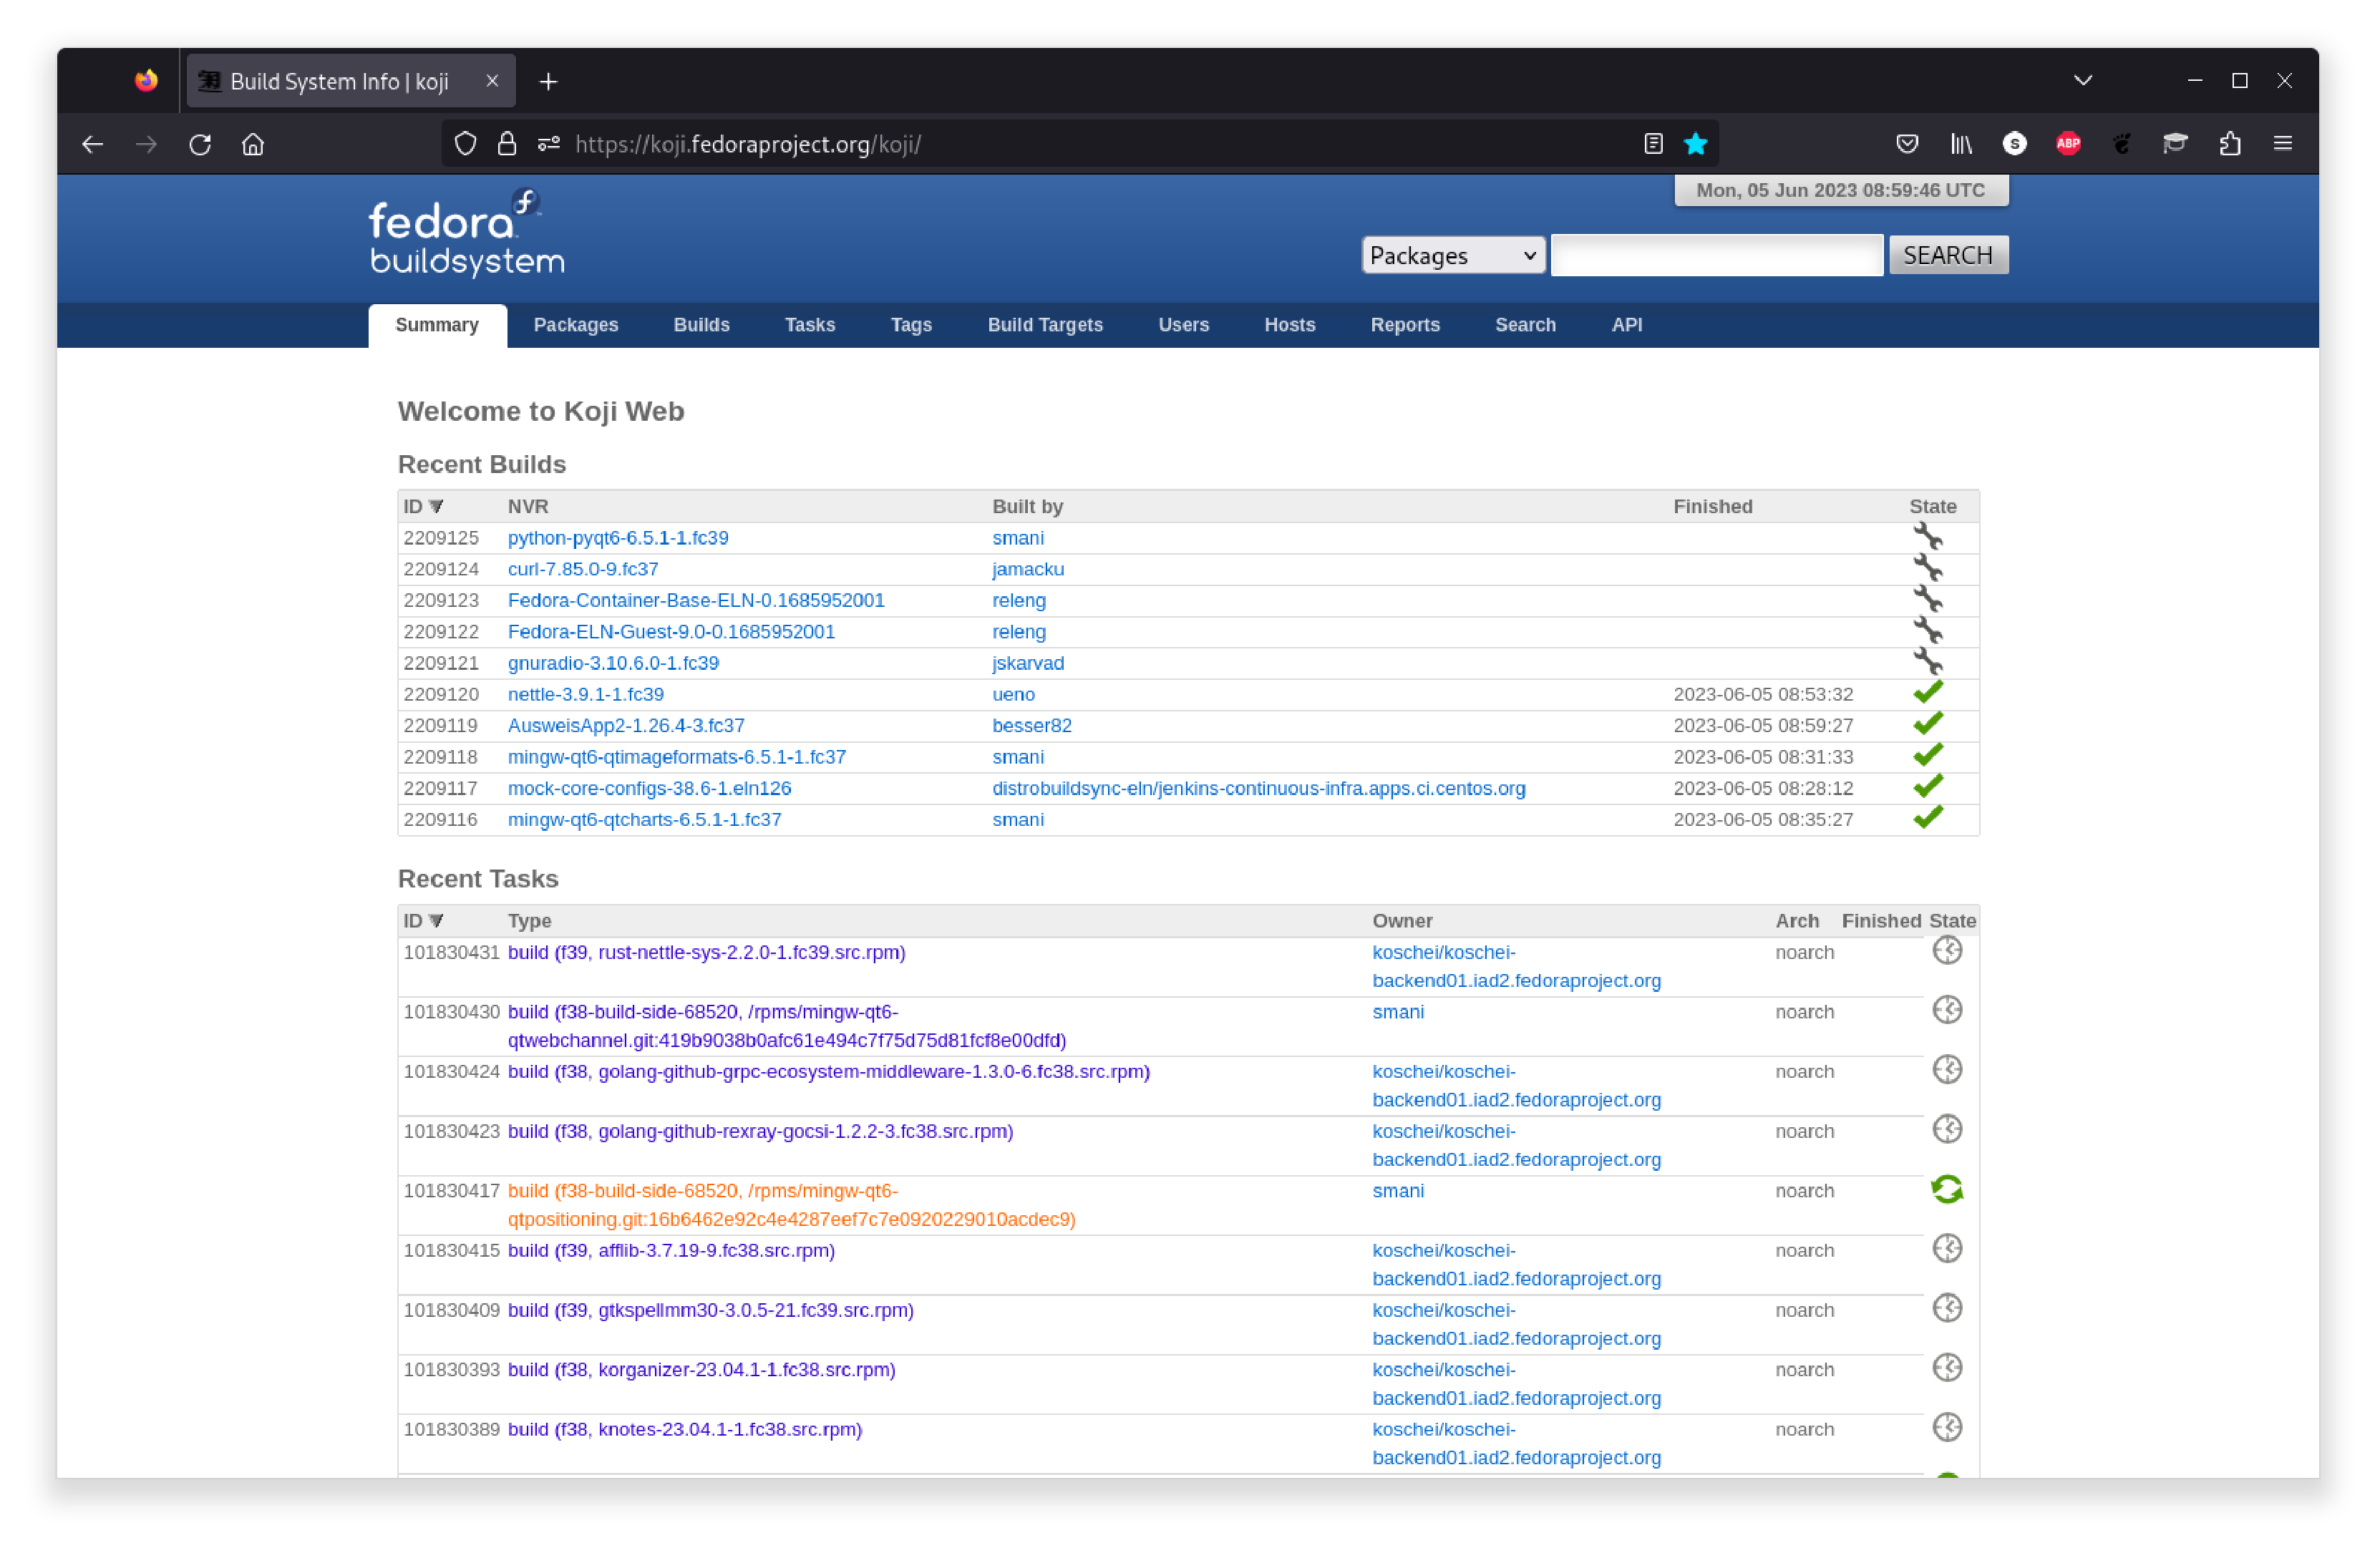
\includegraphics[width=1.0\textwidth,keepaspectratio=true,draft=\ddst]{img/rpms/koji.eps}
\end{center}
Even if your RPM is not distributed by the Fedora project, it possible, if not recommended, to test build your RPM in the Koji environment. \\
To access and use Koji requires to be registered with a Fedora account (see [Sec.~\ref{coprb}]). 
Also to use Koji requires to use the command line. \\[0.25cm]
First of all to start using Koji you need to request a temporary access to the servers by initiating a new Kerberos ticket using your Fedora username and password:
\begin{script}
\fprompt{~} fkinit -u username
Enter your password and OTP concatenated.
(Ignore that the prompt is for only the token)
Password for username@FEDORAPROJECT.ORG: 
\fprompt{~} 
\end{script}
\\[-0.5cm]
\noindent This step is mandatory to allow you to request remote builds on the Koji servers.
\newpage
\noindent To build your RPM using Koji, create the source RPM (if not done already):
\begin{script}
\fprompt{~} \bftt{rpmbuild} \rtt{-bs} program.spec
\end{script}
\\[-0.75cm]
\noindent Then build the RPMs using:
\begin{script}
\fprompt{~} \bftt{koji} \rtt{build} \blue{--sractch rawhide} program-***.fc36.src.rpm
\end{script}
\\[-0.5cm]
\noindent Replace "\texttt{program-***.fc36.src.rpm}" by the name of your SRPM, then press \Enter. 
\begin{script}
\fprompt{~} \bftt{koji} \rtt{build} \blue{--sractch rawhide} program-***.fc36.src.rpm
Uploading srpm:  program-***.src.rpm
[=================================] 100\% 00:00:01   3.14 MiB   2.54 MiB/sec
Created task: 101830239
Task info: \href{https://koji.fedoraproject.org/koji/taskinfo?taskID=101830239}{https://koji.fedoraproject.org/koji/taskinfo?taskID=101830239}
Watching tasks (this may be safely interrupted)...
101830239 build (rawhide, program-***.fc36.src.rpm): free
\end{script}
\\[-0.25cm]
\noindent The link provided in the output of the commands provides you with a webpage to follow the build process:
\begin{center}
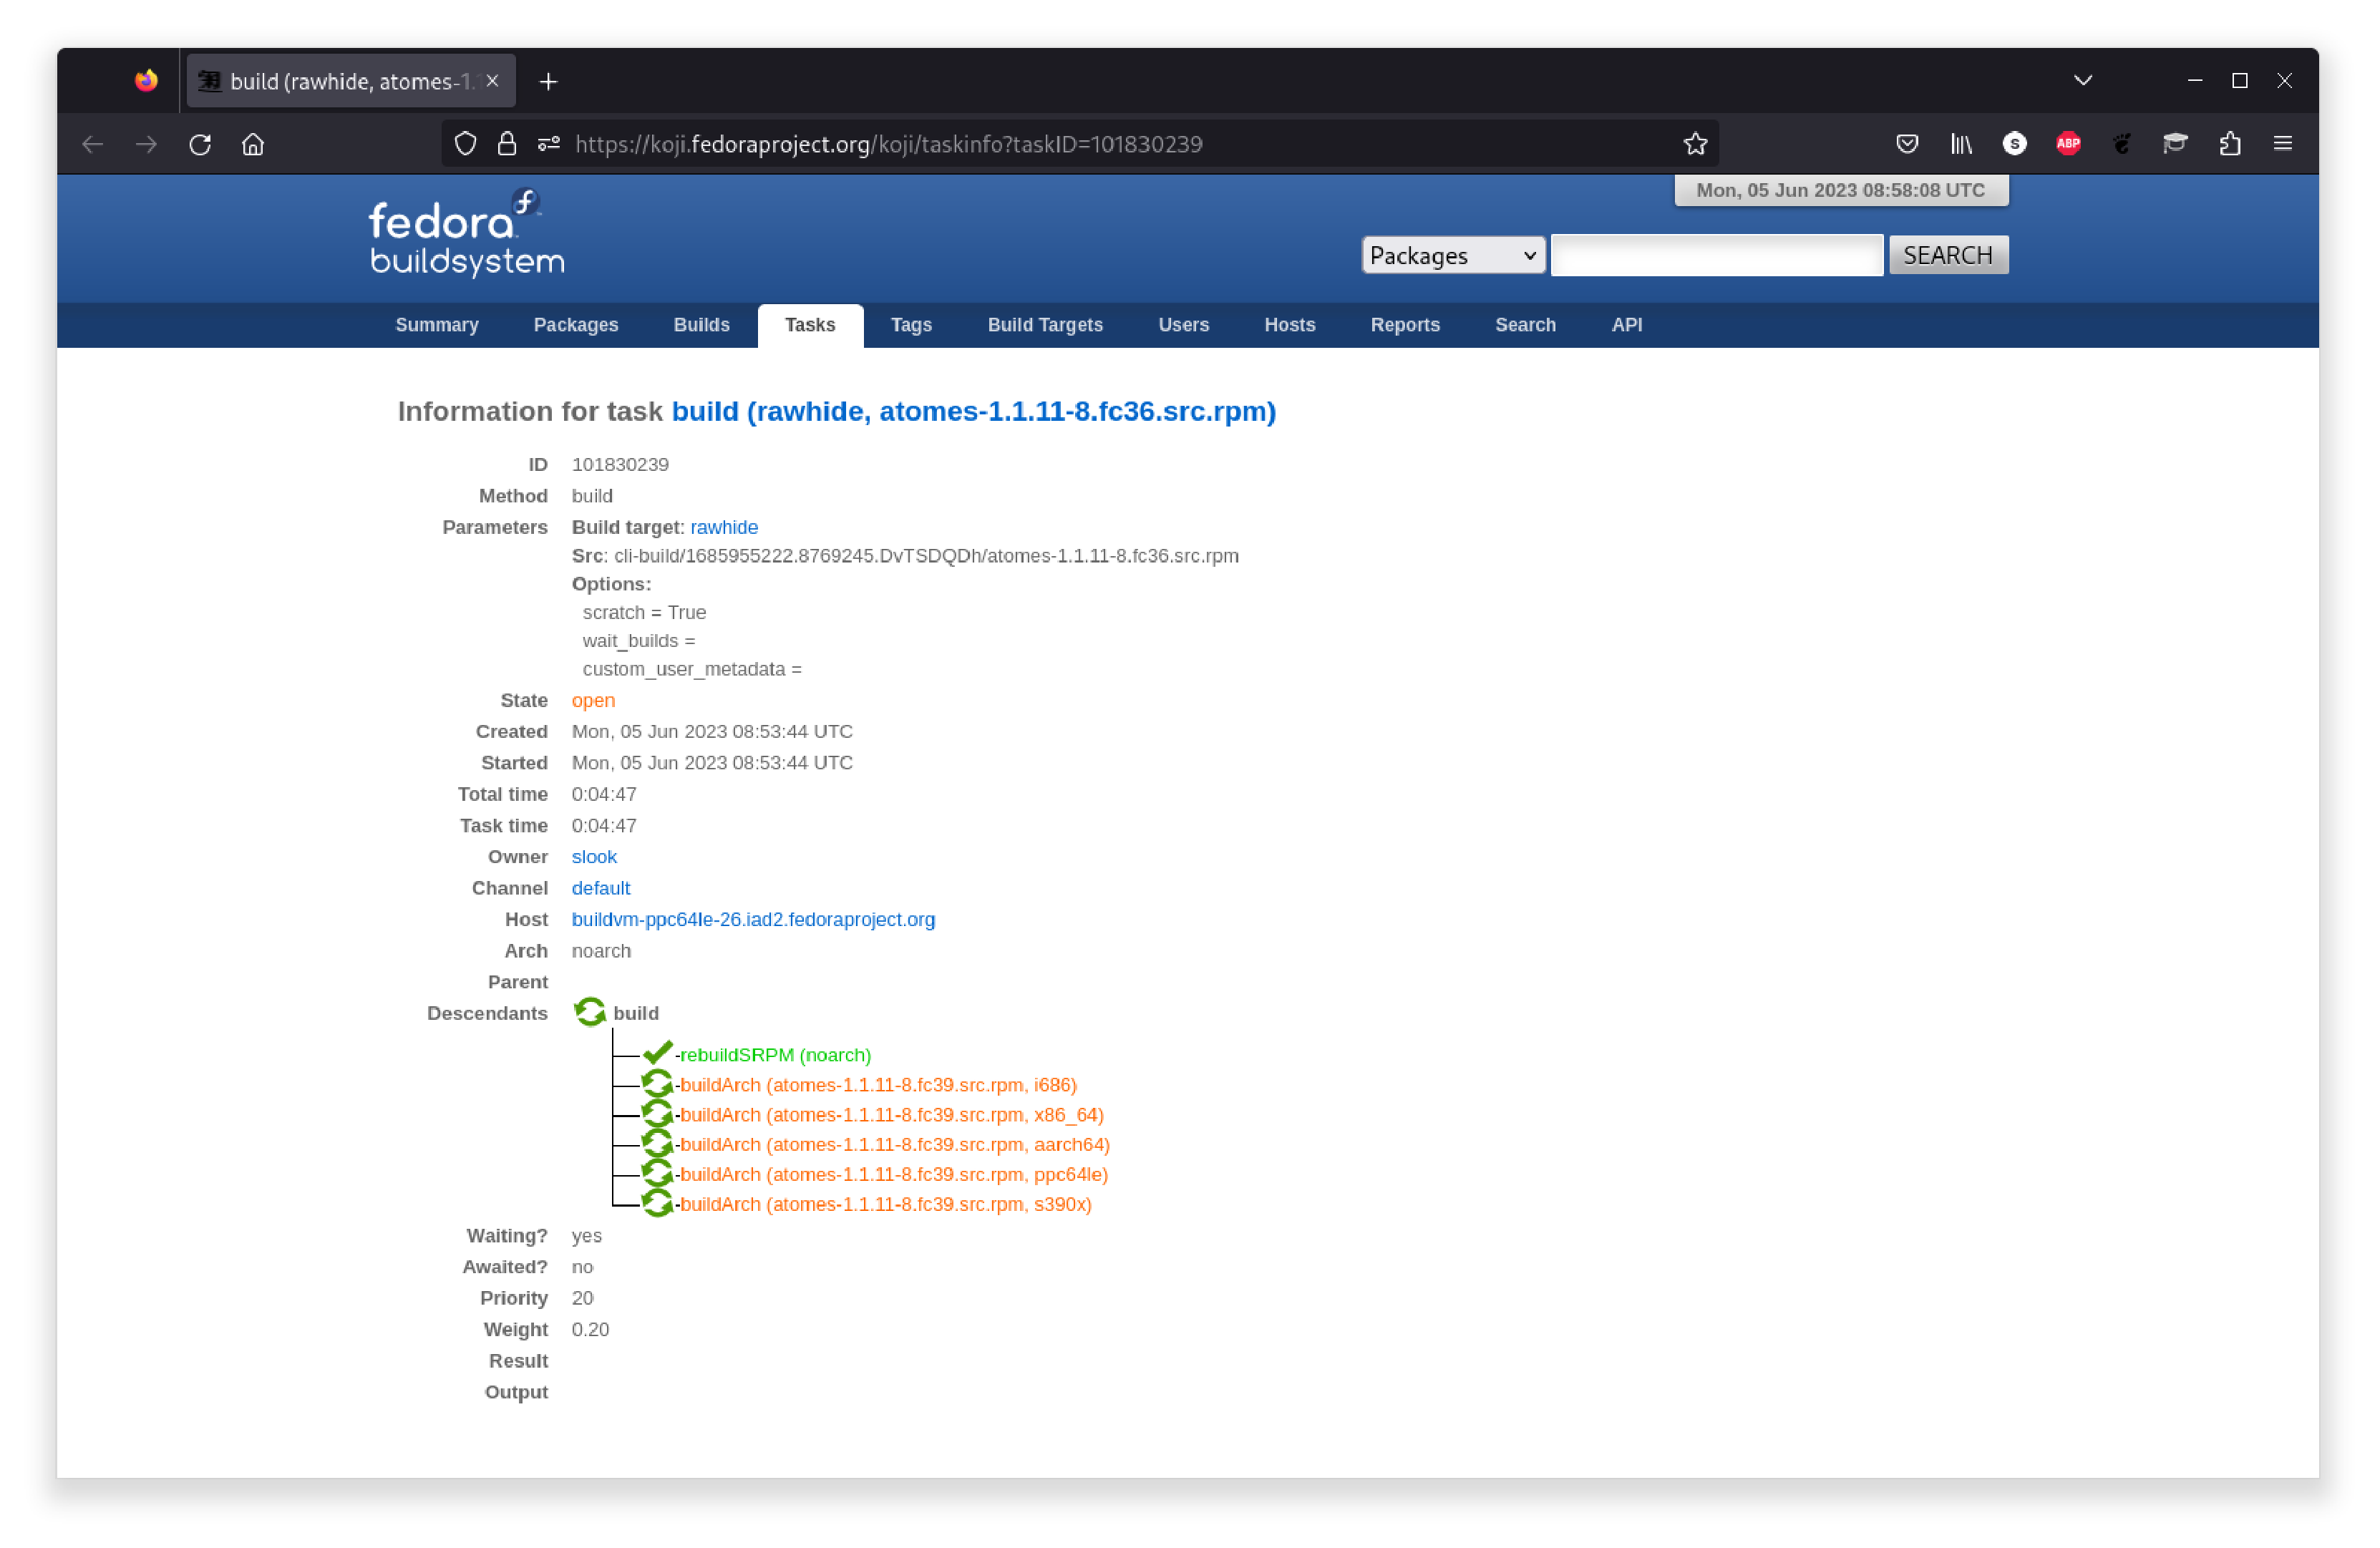
\includegraphics[width=1.0\textwidth,keepaspectratio=true,draft=\ddst]{img/rpms/koji-build.eps}
\end{center}
\newpage
\noindent The information is also provided and refreshed in the terminal:
{\scriptsize{
\begin{script}
\fprompt{~} \bftt{koji} \rtt{build} \blue{--sractch rawhide} program-***.fc36.src.rpm
Uploading srpm:  program-***.src.rpm
[=================================] 100\% 00:00:01   3.14 MiB   2.54 MiB/sec
Created task: 101830239
Task info: \href{https://koji.fedoraproject.org/koji/taskinfo?taskID=101830239}{https://koji.fedoraproject.org/koji/taskinfo?taskID=101830239}
Watching tasks (this may be safely interrupted)...
101830239 build (rawhide, program-***.fc36.src.rpm): free
101830239 build (rawhide, program-***.fc36.src.rpm): free -> open (buildvm-ppc64le-26.iad2.fedoraproject.org)
  101830240 rebuildSRPM (noarch): open (buildvm-ppc64le-02.iad2.fedoraproject.org)
  101830240 rebuildSRPM (noarch): open (buildvm-ppc64le-02.iad2.fedoraproject.org) -> closed
  0 free  1 open  1 done  0 failed
  101830324 buildArch (program-***.src.rpm, i686): free
  101830325 buildArch (program-***.src.rpm, x86\_64): free
\end{script}
}}
\\
\noindent Up to the end of the task:
{\scriptsize{
\begin{script}
\fprompt{~} \bftt{koji} \rtt{build} \blue{--sractch rawhide} program-***.fc36.src.rpm
Uploading srpm:  program-***.src.rpm
[=================================] 100\% 00:00:01   3.14 MiB   2.54 MiB/sec
Created task: 101830239
Task info: \href{https://koji.fedoraproject.org/koji/taskinfo?taskID=101830239}{https://koji.fedoraproject.org/koji/taskinfo?taskID=101830239}
Watching tasks (this may be safely interrupted)...
101830239 build (rawhide, program-***.fc36.src.rpm): free
101830239 build (rawhide, program-***.fc36.src.rpm): free -> open (buildvm-ppc64le-26.iad2.fedoraproject.org)
  101830240 rebuildSRPM (noarch): open (buildvm-ppc64le-02.iad2.fedoraproject.org)
  101830240 rebuildSRPM (noarch): open (buildvm-ppc64le-02.iad2.fedoraproject.org) -> closed
  0 free  1 open  1 done  0 failed
  101830324 buildArch (program-***.src.rpm, i686): free
  101830325 buildArch (program-***.src.rpm, x86\_64): free
  101830328 buildArch (program-***.src.rpm, s390x): free
  101830326 buildArch (program-***.src.rpm, aarch64): open (buildvm-a64-31.iad2.fedoraproject.org)
  101830327 buildArch (program-***.src.rpm, ppc64le): free
  101830324 buildArch (program-***.src.rpm, i686): free -> open (buildvm-x86-19.iad2.fedoraproject.org)
  101830328 buildArch (program-***.src.rpm, s390x): free -> open (buildvm-s390x-21.s390.fedoraproject.org)
  101830325 buildArch (program-***.src.rpm, x86\_64): free -> open (buildvm-x86-12.iad2.fedoraproject.org)
  101830327 buildArch (program-***.src.rpm, ppc64le): free -> open (buildvm-ppc64le-17.iad2.fedoraproject.org)
  101830326 buildArch (program-***.src.rpm, aarch64): open (buildvm-a64-31.iad2.fedoraproject.org) -> closed
  0 free  5 open  2 done  0 failed
  101830328 buildArch (program-***.src.rpm, s390x): open (buildvm-s390x-21.s390.fedoraproject.org) -> closed
  0 free  4 open  3 done  0 failed
  101830324 buildArch (program-***.src.rpm, i686): open (buildvm-x86-19.iad2.fedoraproject.org) -> closed
  0 free  3 open  4 done  0 failed
  101830325 buildArch (program-***.src.rpm, x86\_64): open (buildvm-x86-12.iad2.fedoraproject.org) -> closed
  0 free  2 open  5 done  0 failed
  101830327 buildArch (program-***.src.rpm, ppc64le): open (buildvm-ppc64le-17.iad2.fedoraproject.org) -> closed
  0 free  1 open  6 done  0 failed
101830239 build (rawhide, program-***.src.rpm): open (buildvm-ppc64le-26.iad2.fedoraproject.org) -> closed
  0 free  0 open  7 done  0 failed

101830239 build (rawhide, program-***.src.rpm) completed successfully
\end{script}
}}

\newpage
\subsection{Testing the RPM}
\label{rpmtesting}

Up to this point I introduced the different ways to build a RPM, leaving apart possible failures and errors. 
However if you intend to distribute your RPM, even if not by the official Fedora software repositories, it is important to know 
how to check for possible issues. In particular because even a successful build can contain errors.  
Also, not surprisingly, the first step in getting your RPM distributed by Red Hat is to get rid of 
a comprehensive list of possible errors. 

\subsubsection{Locally using the command line}

To test your RPM via the command line use:
\begin{itemize}
\item Check the RPM using the \bftt{rpmlint} command:
\begin{itemize}
\item On the "\bftt{.spec}" file:
\begin{scriptii}
\fprompt{~} \bftt{rpmlint} \rtt{-v} program.spec
\end{scriptii}
\item On the SRPM:
\begin{scriptii}
\fprompt{~} \bftt{rpmlint} \rtt{-v} program*.src.rpm 
\end{scriptii}
\item On the RPM:
\begin{scriptii}
\fprompt{~} \bftt{rpmlint} \rtt{-v} program*.rpm 
\end{scriptii}
\end{itemize}
\item Check the file permissions in the RPM using the \bftt{rpmls} command:
\begin{scripti}
\fprompt{~} \bftt{rpmls} program*.rpm
\end{scripti}
\item Mock build and review of the RPM using the \bftt{fedora-review} tool. 
\begin{scripti}
\fprompt{~} \bftt{fedora-review} \rtt{-n} program
\end{scripti}
\\[-1cm]
\noindent Where \texttt{program} is the name of the "\bftt{.spec}" file, without the \texttt{.spec} extension. \\
Both \texttt{program.spec} and the source RPM must be located in the active directory. \\
\newpage
\noindent Equivalent to: 
\begin{scripti}
\fprompt{~} \bftt{fedora-review} \rtt{--rpm-spec -n} program*.src.rpm
\end{scripti}
\\[-1cm]
\noindent Where is \texttt{program*.src.rpm} is the source rpm, note that in this case \texttt{fedora-review} uses the spec file inside the source rpm. \\[0.25cm]
\texttt{fedora-review} will output the results of the analysis in a directory with the program name. 
\end{itemize}
These commands produce both errors and warnings. \\
It is mandatory to fix all errors to distribute your RPM, while some warning can be safely ignored. 

\subsubsection{Remotely on Copr}
\label{rcopr}

You can activate review tools on Copr to get a lot of information on the build, when creating a new project or editing the project settings:
\begin{center}
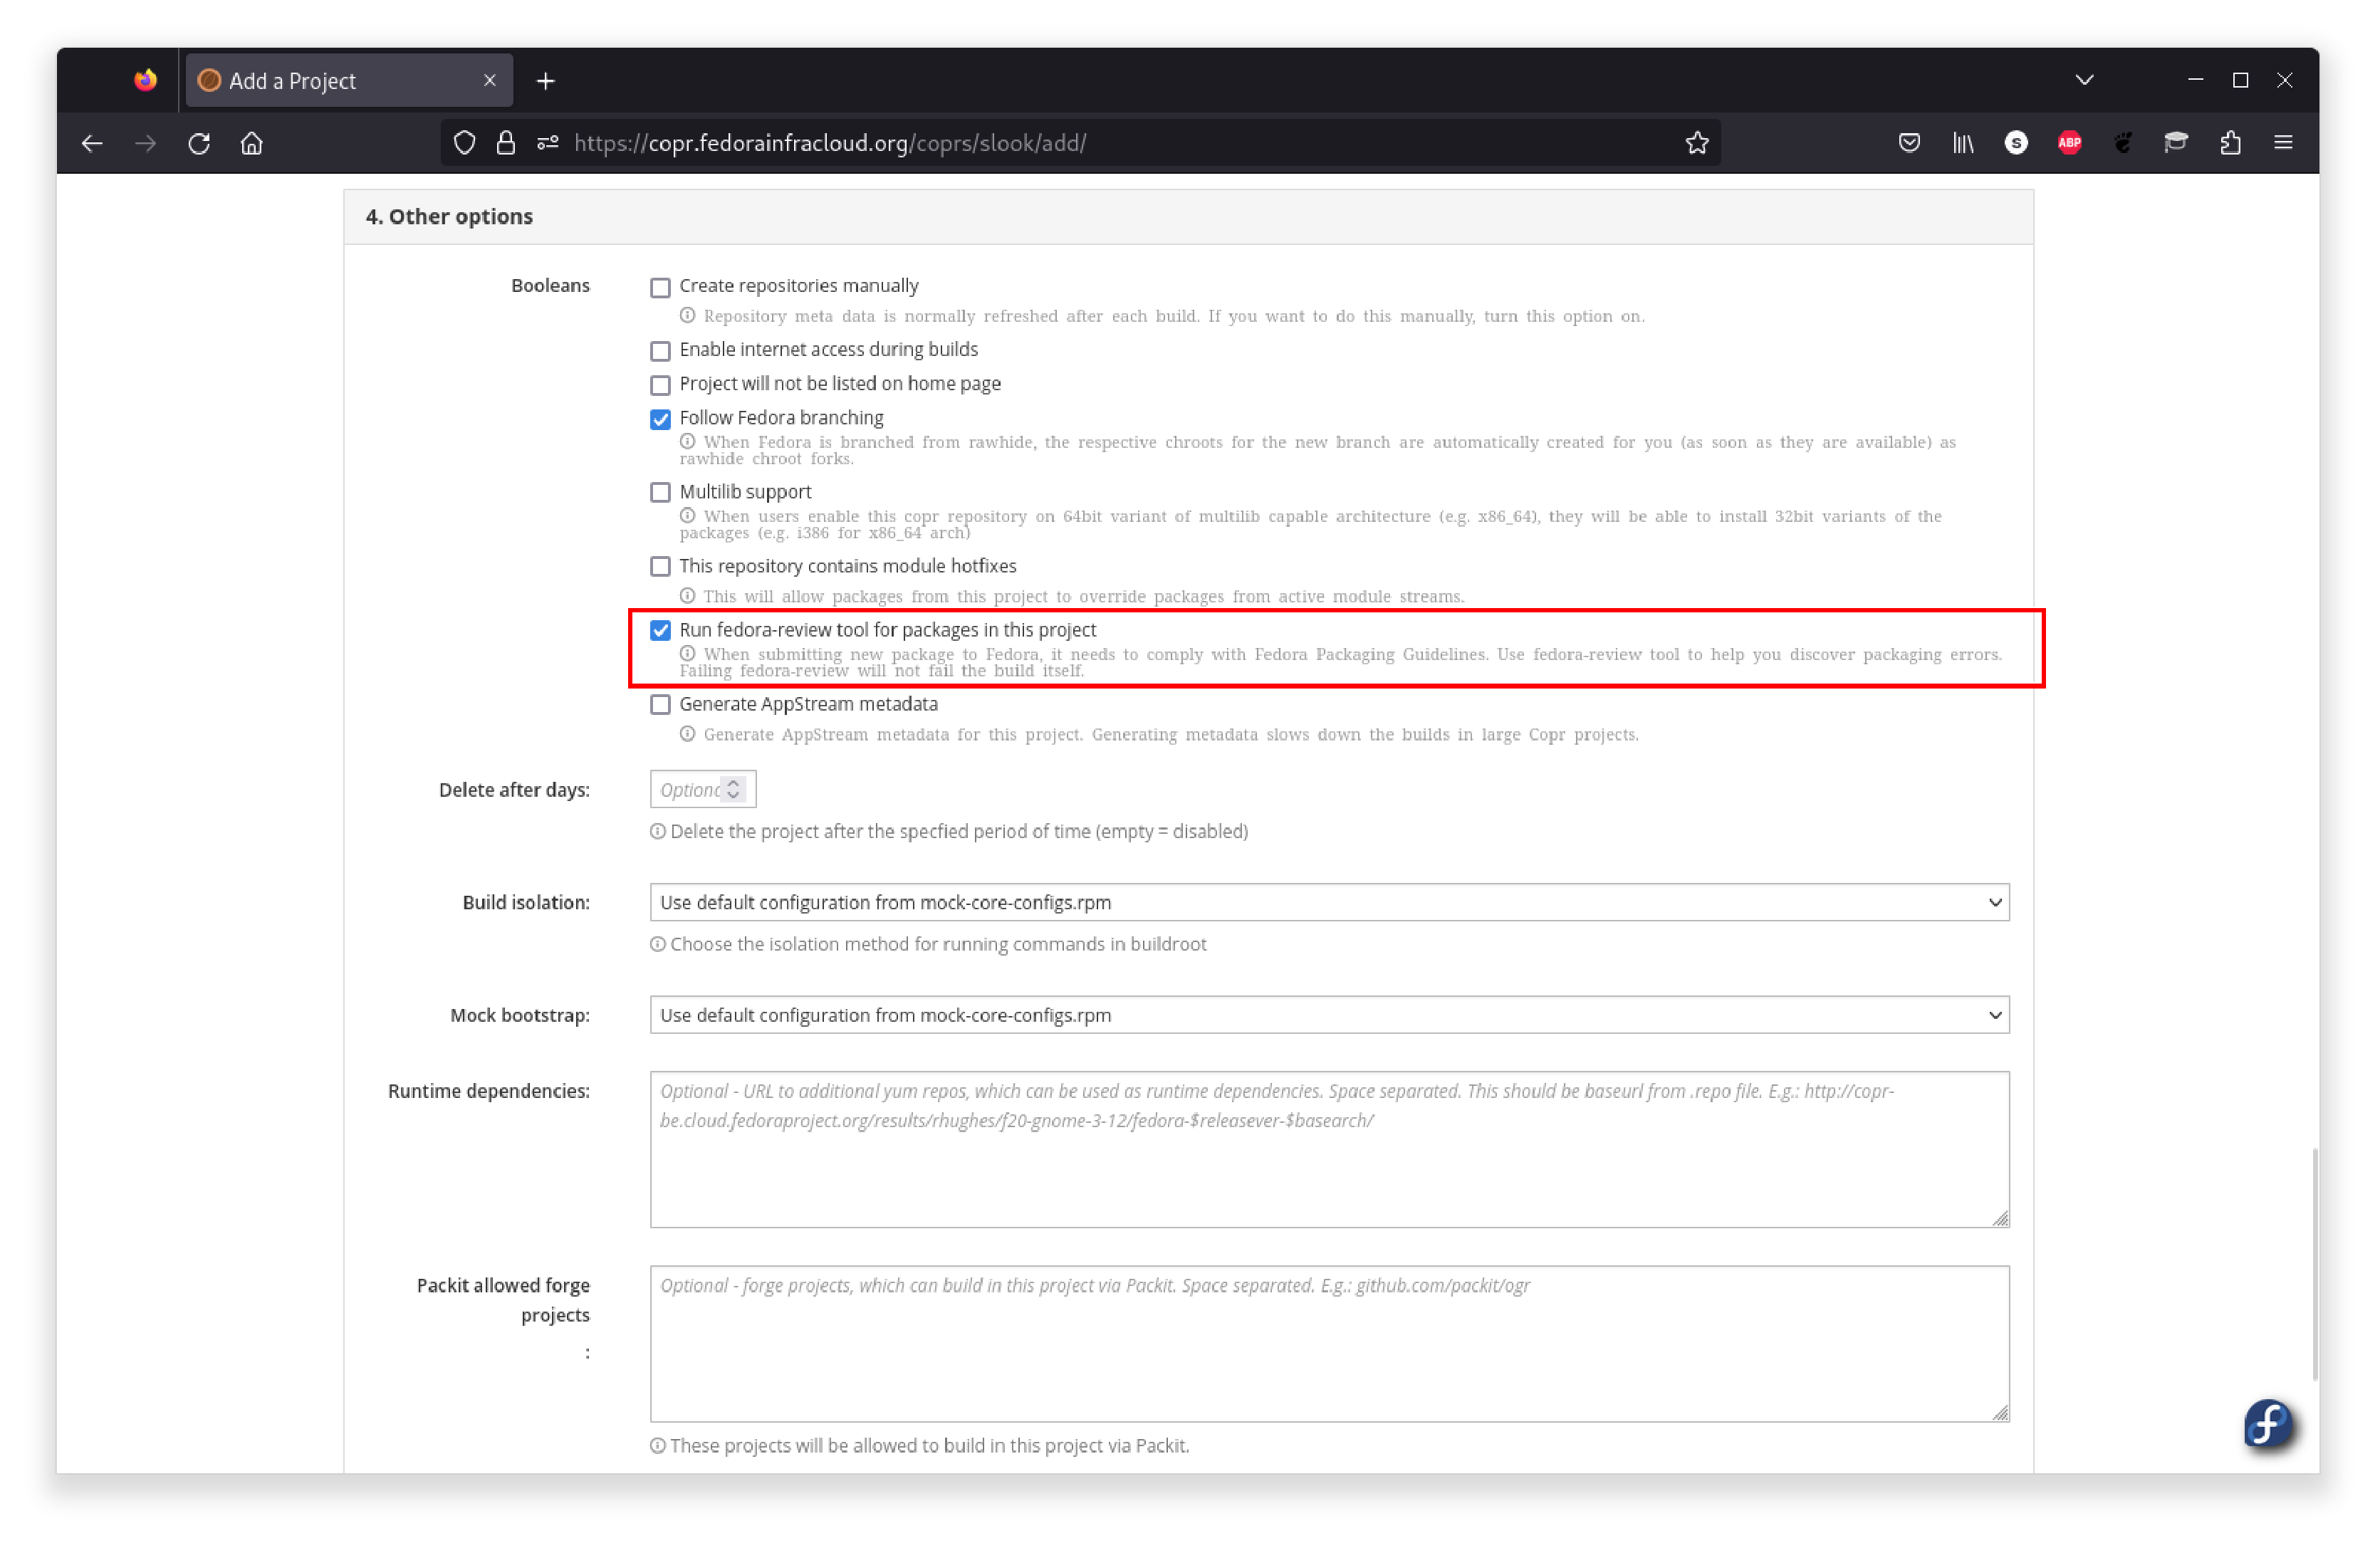
\includegraphics[width=1.0\textwidth,keepaspectratio=true,draft=\ddst]{img/rpms/copr-review.eps}
\end{center}
\newpage
\noindent After the building the RPM with the proper option, check out the results and open the corresponding information page: \\
\begin{center}
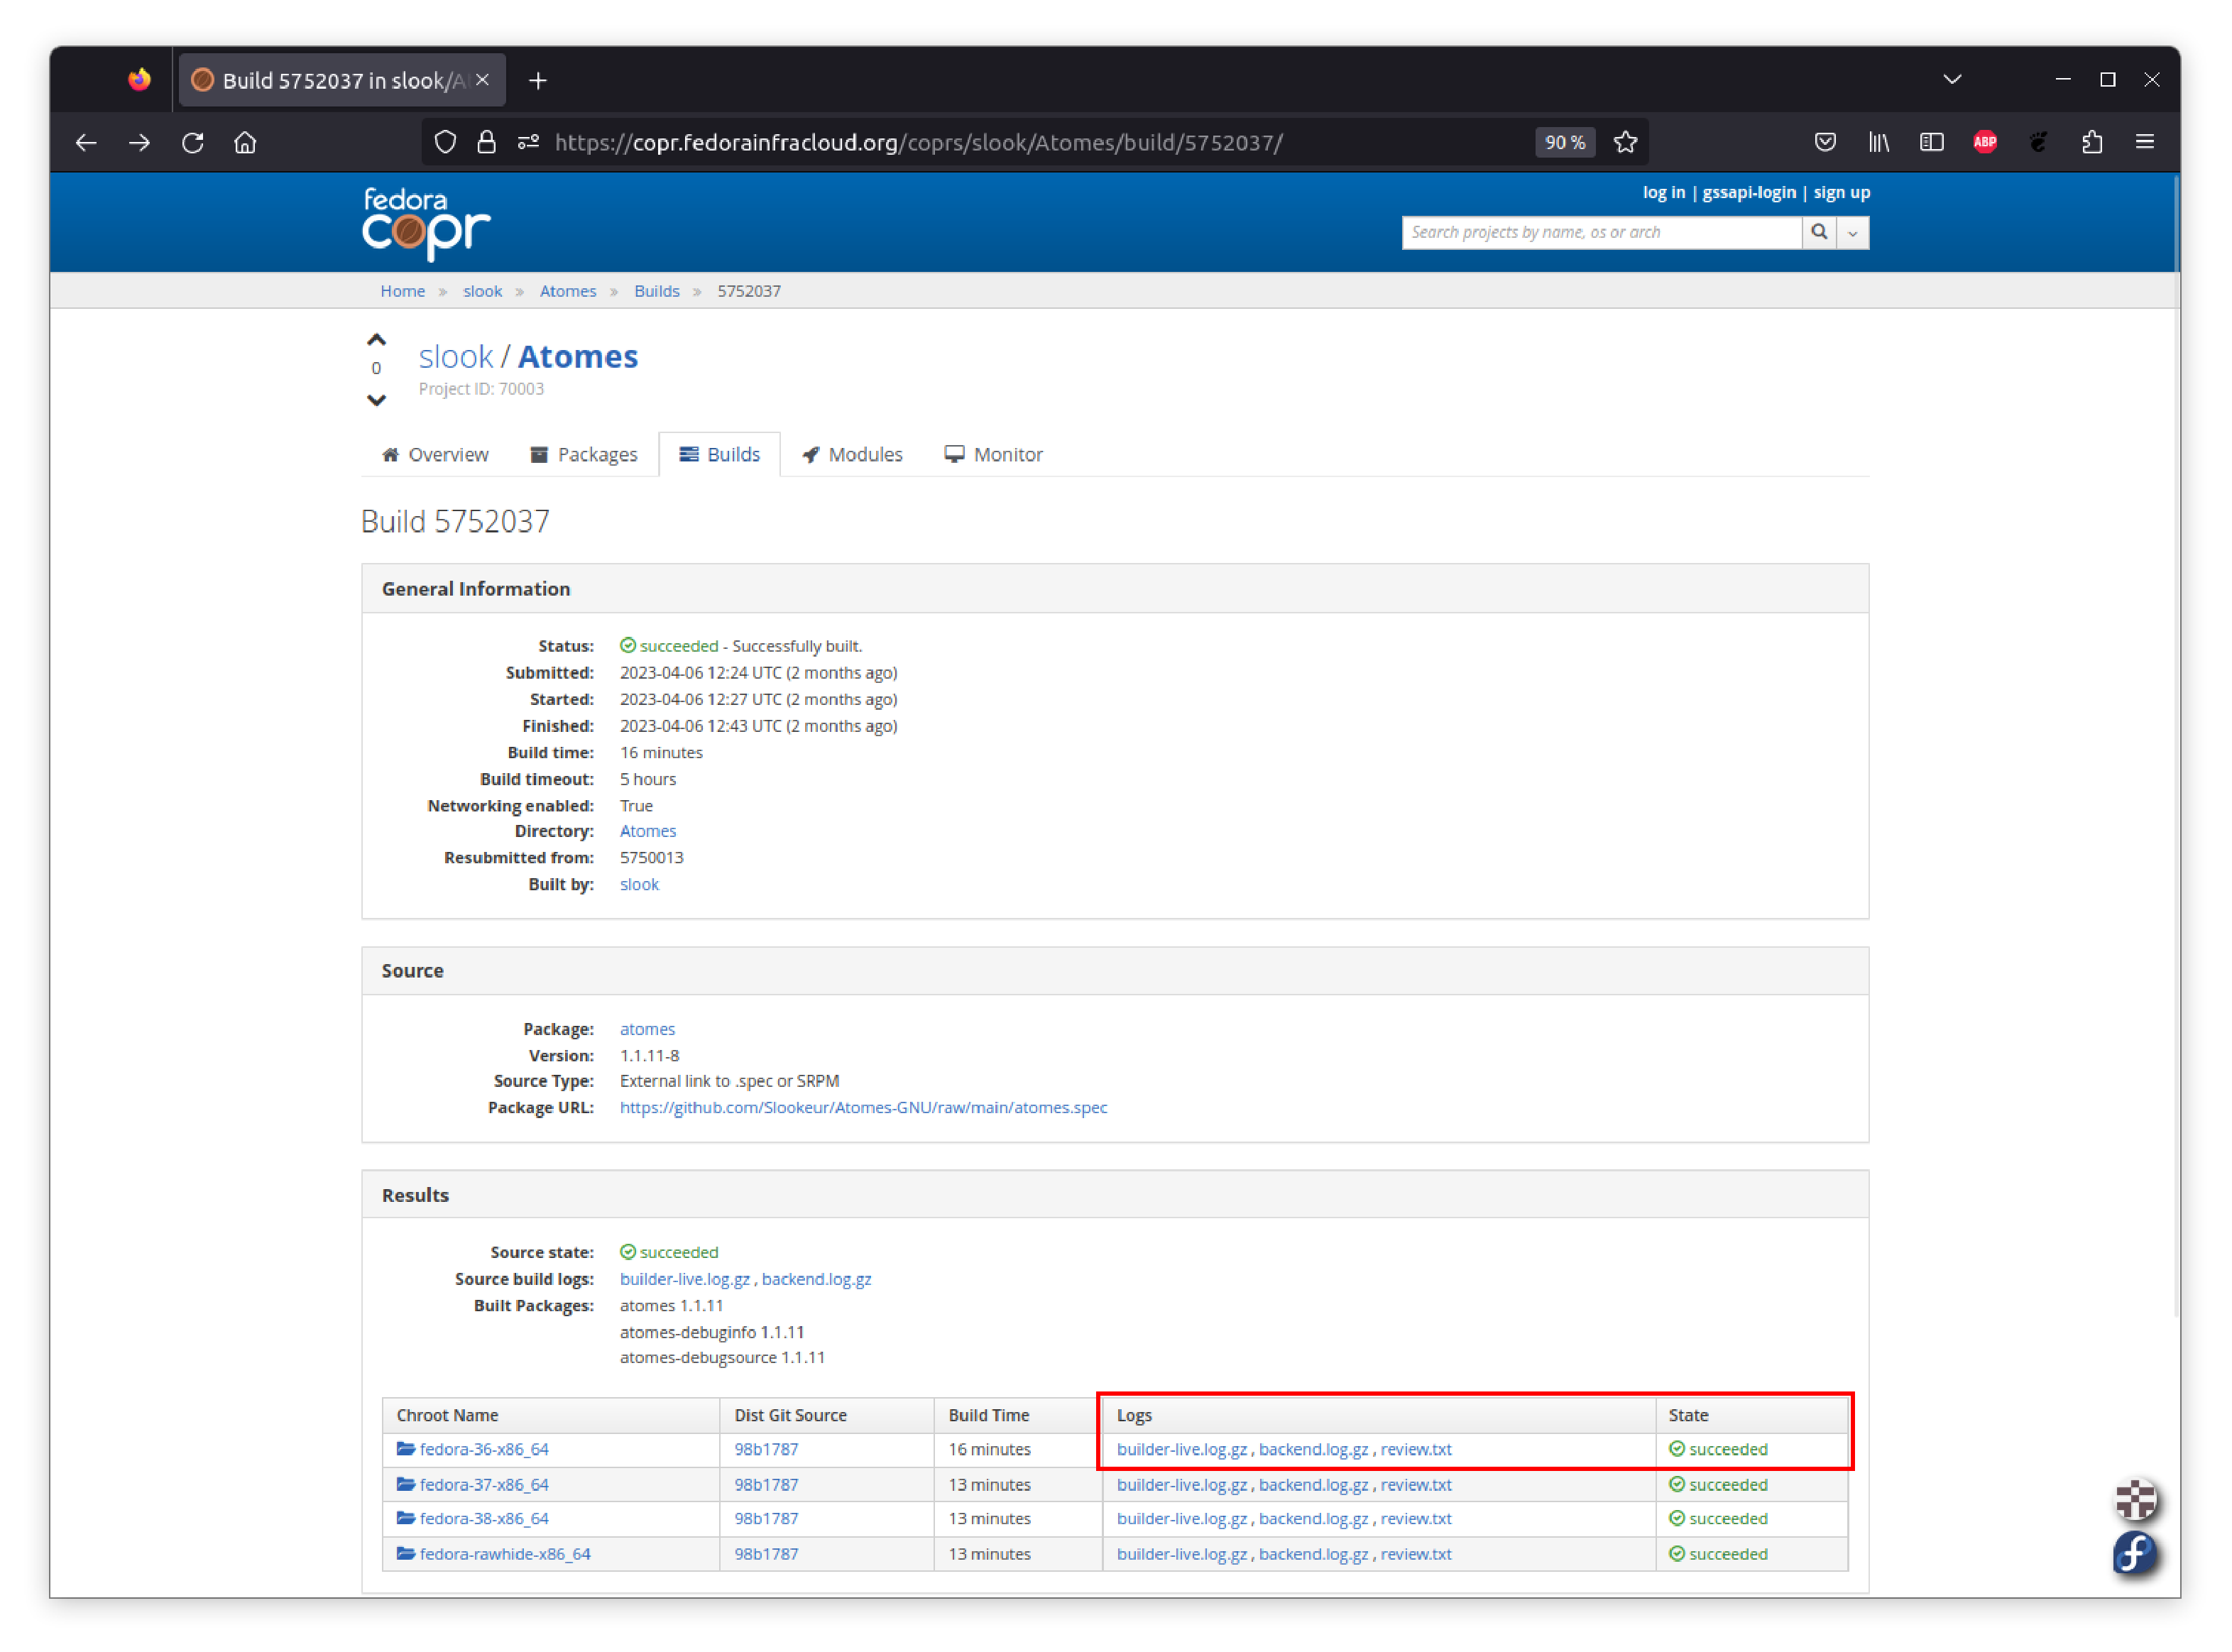
\includegraphics[width=0.8\textwidth,keepaspectratio=true,draft=\ddst]{img/rpms/copr-rev-res.eps}
\end{center}
Scroll down if needed, and in the bottom section check the "Logs" section, several files outputs of the build are provided, including a file "\texttt{review.txt}", 
click on the link to access the results of the Fedora review:
\begin{center}
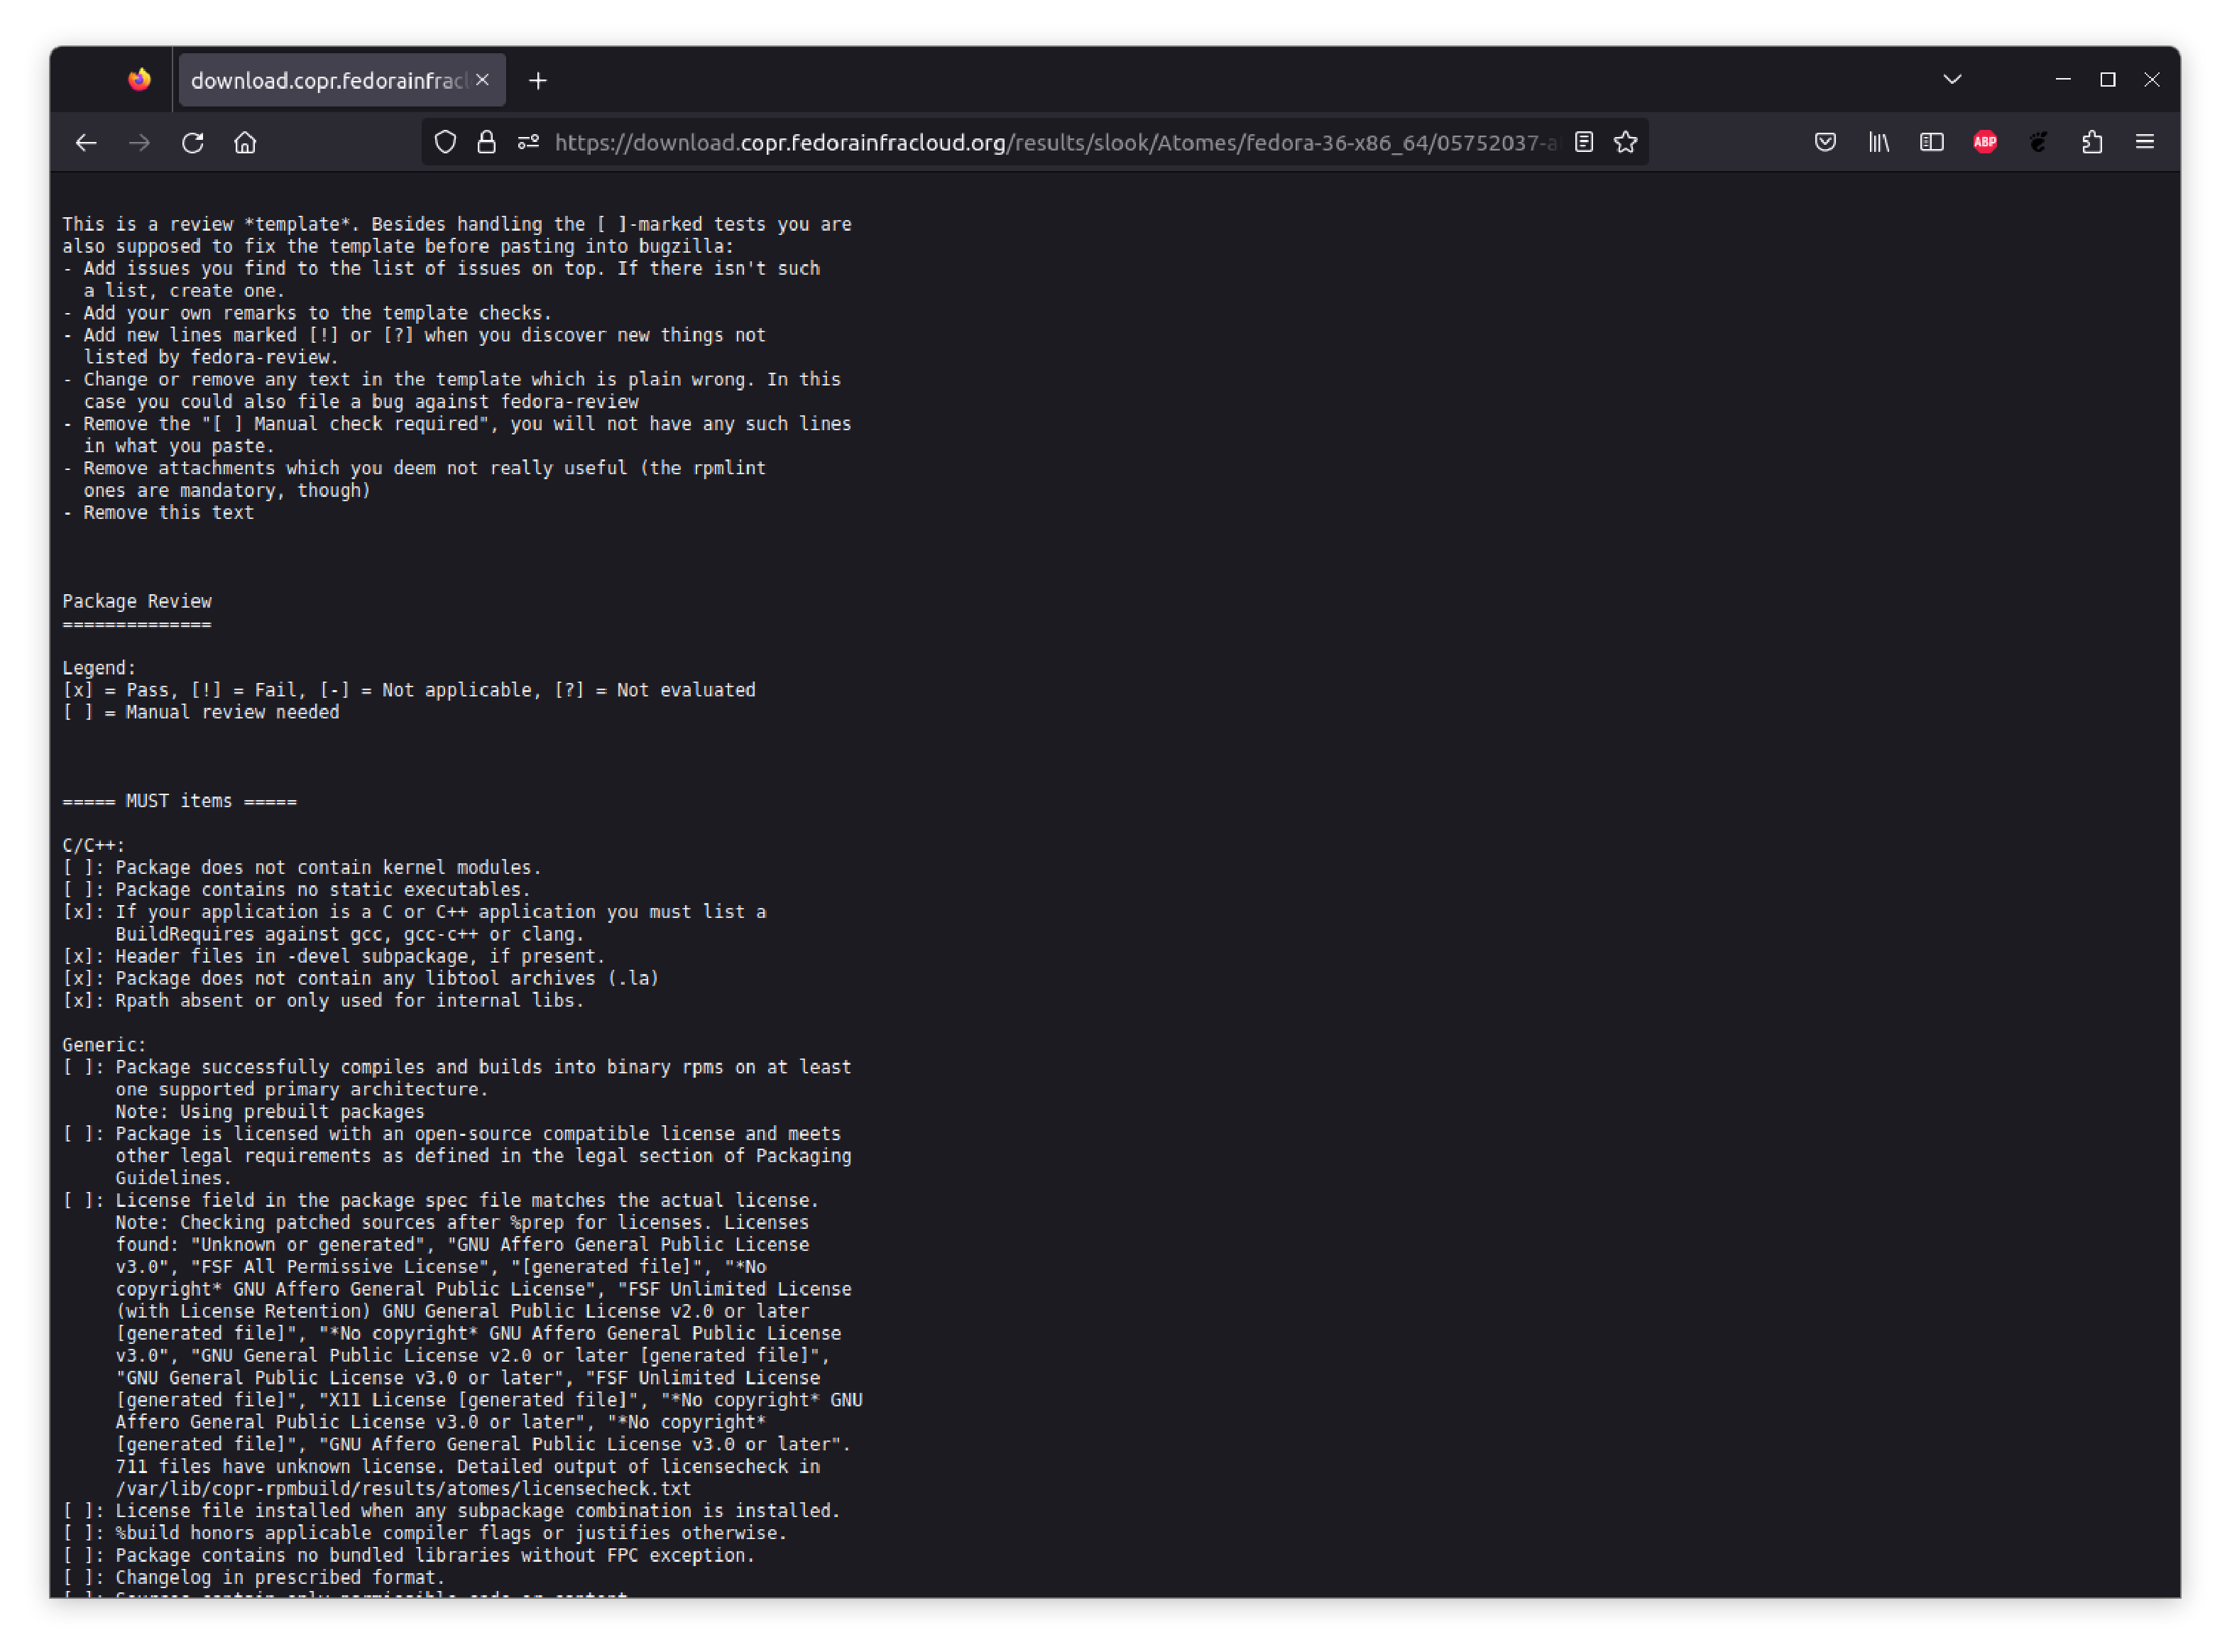
\includegraphics[width=0.8\textwidth,keepaspectratio=true,draft=\ddst]{img/rpms/copr-package-review.eps}
\end{center}

%\subsubsection{Remotely on Koji}
%\label{rkoji}
%On Koji review information are accessible following the link provide at the beginning of the output:
%\begin{script}
%\fprompt{~} \bftt{koji} \rtt{build} --sractch rawhide program-***.fc36.src.rpm
%Uploading srpm:  program-***.src.rpm
%[=================================] 100\% 00:00:01   3.14 MiB   2.54 MiB/sec
%Created task: 101830239
%Task info: \href{https://koji.fedoraproject.org/koji/taskinfo?taskID=101830239}{https://koji.fedoraproject.org/koji/taskinfo?taskID=101830239}
%\end{script}
%Simply open the link: \texttt{\href{https://koji.fedoraproject.org/koji/taskinfo?taskID=101830239}{https://koji.fedoraproject.org/koji/taskinfo?taskID=101830239}} \\[0.25cm]
%Then scroll down on this page up to the build information, select (click) on one the build architectures to check the 

\subsection{Submitting your RPM to the Fedora project}

At this point I will consider that you already prepared you own version of the RPM package, ideally following the guidelines provided in this manual. 
If not you should really take the time to prepare a first, raw, version of your RPM package. 
Doing so will at least tell the Fedora packagers, members of the Fedora community 
in charge of packaging applications, that you are willing to be part of the process, as you should. \\[0.25cm]
Ideally you should already have test build this package in Copr and / or Koji:
\begin{itemize}
\item For Copr copy the link to the package review information (see [Sec.~\ref{rcopr}]).
\item For Koji copy the address of the webpage with the build information (see [Sec.~\ref{kojib}]). 
\end{itemize}
To submit your RPM package to the Fedora project:
\begin{enumerate}
\item Create a \href{https://accounts.fedoraproject.org/}{Fedora account} (see [Sec.~\ref{coprb}]).
\item Create a \href{https://bugzilla.redhat.com}{Red Hat Bugzilla} account, with the same email used to create the Fedora account. 
%\begin{center}
%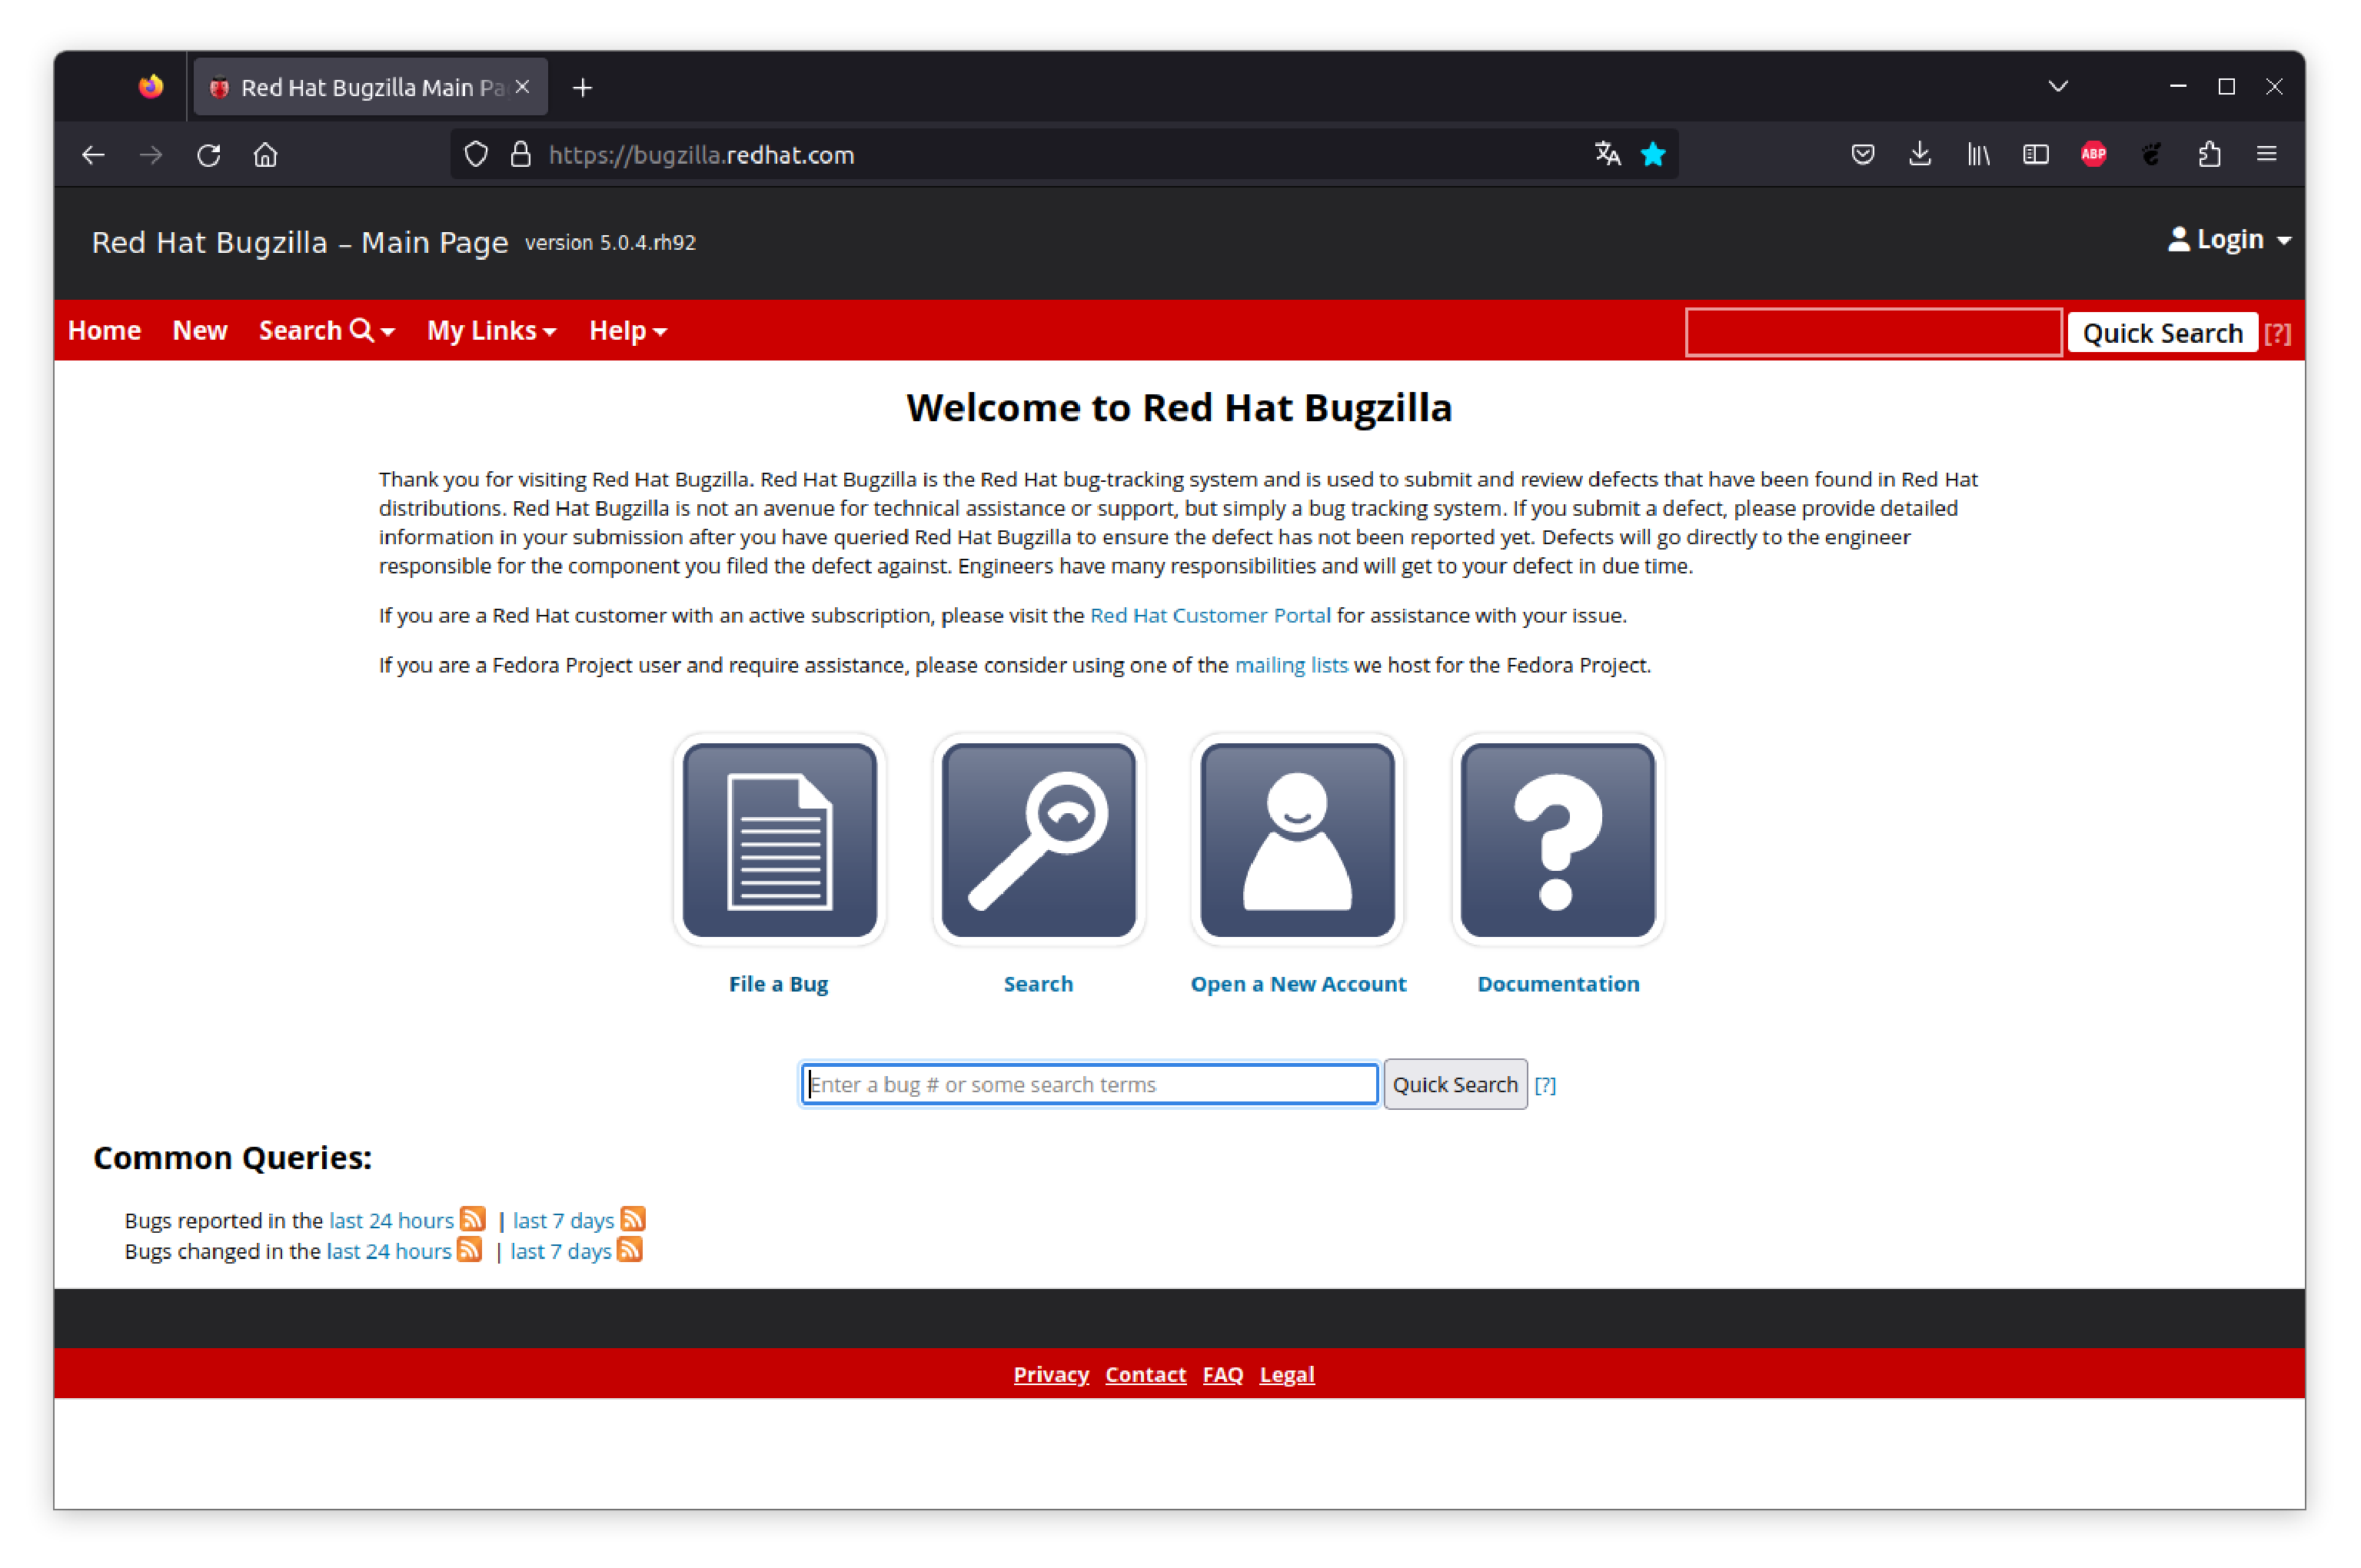
\includegraphics[width=1.0\textwidth,keepaspectratio=true,draft=\ddst]{img/rpms/bugzilla/bugzilla-0.eps}
%\end{center}
\item Create a message in \href{https://bugzilla.redhat.com/}{https://bugzilla.redhat.com/} to request the review of your package. 
\item Create a message to introduce yourself and ask to join the Fedora Package Maintainers.
%More information here: \href{https://docs.fedoraproject.org/en-US/package-maintainers/Joining\_the\_Package\_Maintainers/}{https://docs.fedoraproject.org/en-US/package-maintainers/Joining\_the\_Package\_Maintainers/}
\end{enumerate}

\subsubsection{The Red Hat Bugzilla message to request a new package review}

\begin{enumerate}
\item Login to \href{https://bugzilla.redhat.com}{Red Hat Bugzilla}
\begin{center}
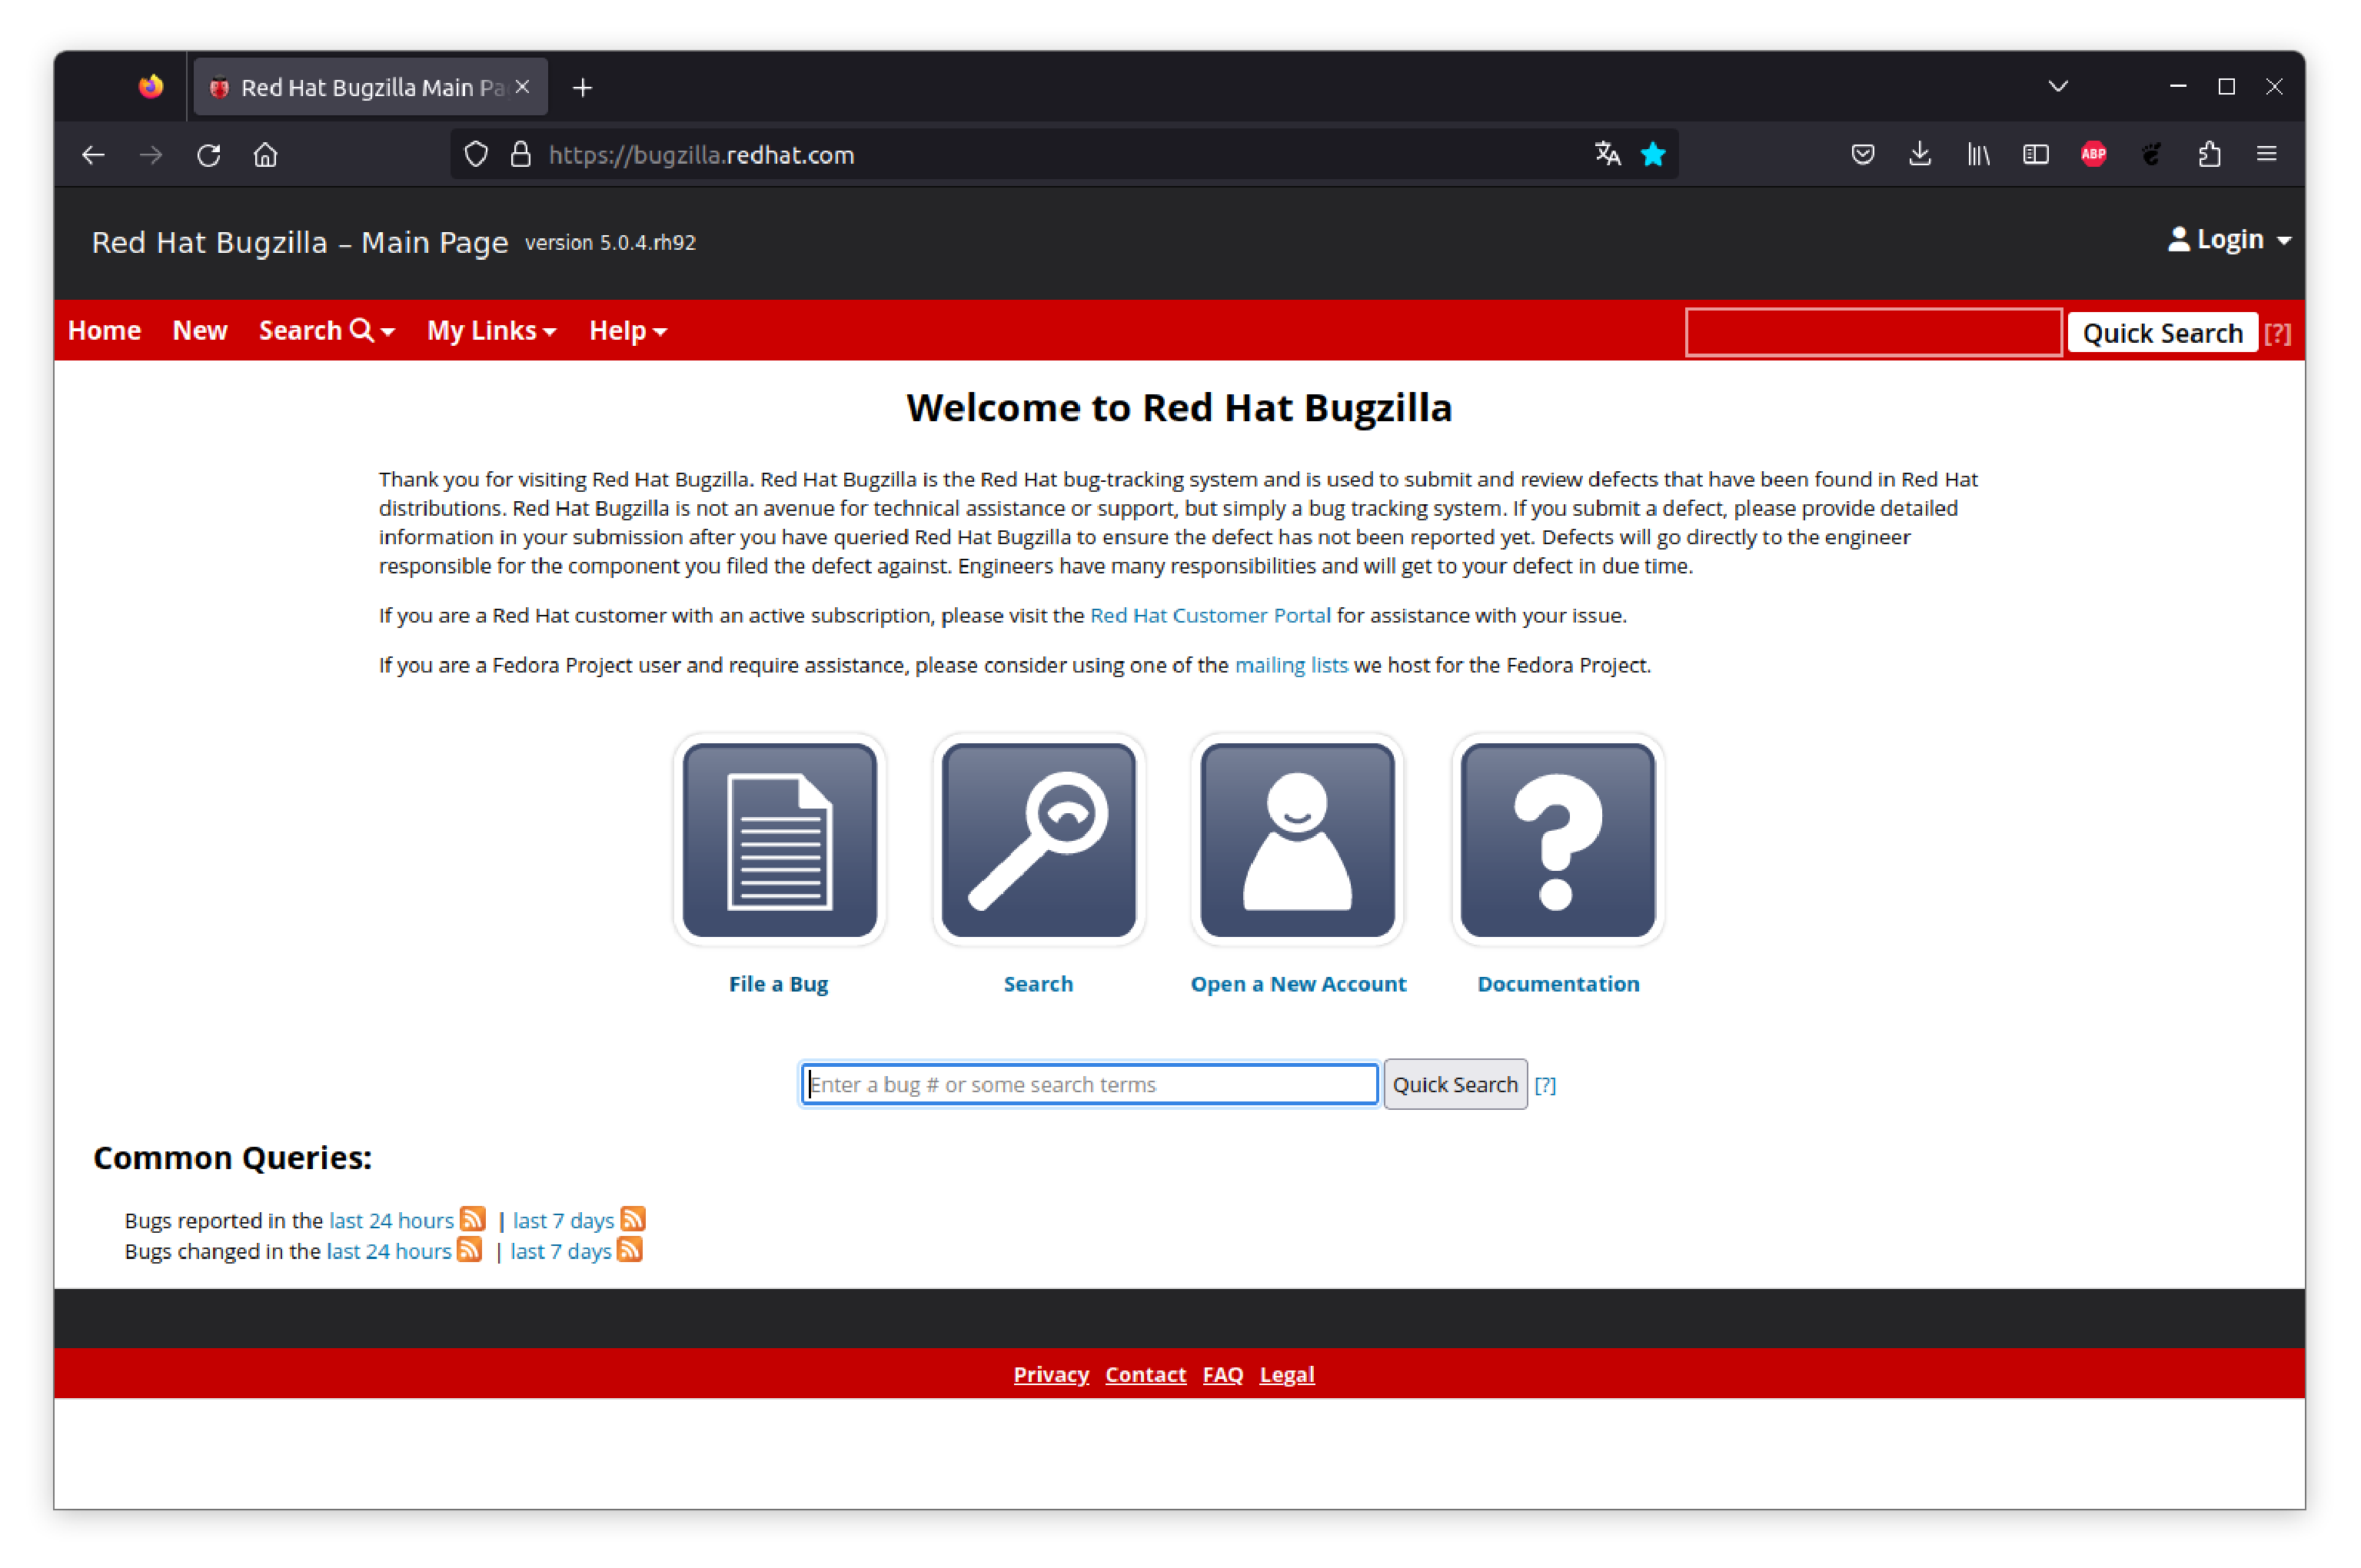
\includegraphics[width=0.9\textwidth,keepaspectratio=true,draft=\ddst]{img/rpms/bugzilla/bugzilla-0.eps}
\end{center}
The click of "File a Bug", please note that depending if you logged in using your "Fedora Account System" or a "Red Hat Bugzilla Account" the page dedicated to the preparation of the bug message might be slightly different. \\
For the sake of consistency with this tutorial I would recommend to login using the "Red Hat Bugzilla" account you just created. 
\item Then "File a Bug" and create a new message: 
\begin{itemize}
\item Click of "Fedora", then click of "Fedora" again:
\begin{center}
\hspace{-3.25cm}
\includegraphics[width=1.05\textwidth,keepaspectratio=true,draft=\ddst]{img/rpms/bugzilla/bugzilla-4.eps}
\end{center}
You are now of the interface dedicated to the preparation of the message to ask for your package to be reviewed by members of the Fedora Package Maintainers.
\item In Component select (or enter) "\texttt{Package Review}" 
\item Summary should start with:\\[0.25cm]
"\texttt{Review request: program - short description}"\\[-0.4cm]
\begin{itemize}
\item \texttt{program} is the name of your program / package.\\[0.25cm]
It is the name that will be used to create the Fedora package, and it is case sensitive, 
so choose it carefully, basically this is the keyword Fedora, and Red Hat based Linux, users will use to search for and install your program using: \\[-0.75cm]
\begin{scriptiii}
\fprompt{~} sudo dnf install prog
\end{scriptiii}
\\[-0.75cm]
\item \texttt{short description} describes its purpose in as few words as possible\\[-0.25cm] 
\end{itemize}
\item Priority, Hardware and OS should be set to "\texttt{Unspecified}" 
\item Severity should be set to "\texttt{Medium}"
\item In the message section, you can delete the "\texttt{Bug Description}" section since your are not reporting a bug, instead you are asking for help to review your new package: 
\begin{itemize}
\item In the introduction part of the message: 
\begin{itemize}
\item Introduce yourself:
\begin{itemize}
\item Real name
\item Fedora Account System username (useful for future exchanges)
\item Tell more about your work. \\[0.25cm]
Doing this professionally it is a good idea to tell Package Maintainers about your job,
indeed it is likely to help you find people in the same area of expertise, the best way to get help and to find a sponsor (see below). \\[-0.25cm] 
\item Introduce briefly your software\\[-0.25cm]
\end{itemize}
\item Provide a link to the repository of the "\texttt{.spec}" file used to create the RPM. 
\item Provide a link to the last SRPM (source RPM).
\item Ideally provide a link to the last successful Koji (or Copr) build. 
\item State that you need a sponsor: this is mandatory for your first package. \\[0.25cm]
A sponsor is an official member of the Fedora Package Maintainers experienced enough to ensure that your package 
is properly prepared, and who can validate its integration to the Fedora ecosystem. 
Your sponsor will also register you as an official Fedora Package Maintainer for your package. \\
\end{itemize}
\item In the Description part of the message:
\begin{itemize}
\item Describe your program with details. 
\item Describe the interest of the program for the community.
\end{itemize}
\end{itemize}
\end{itemize}
\newpage
\item Test the information your provided in your bug "Package review" message: \\[0.25cm]
Once the email has been sent you will receive a link to a webpage hosting the entire discussion on \href{https://bugzilla.redhat.com}{Red Hat Bugzilla} at the address: \\[0.25cm]
\texttt{https://bugzilla.redhat.com/show\_bug.cgi?id=}\dctt{???????} \\[0.25cm]
\noindent Where \dctt{???????} is the bug message id number that you will find on the email you received and on the webpage hosting the discussion. \\
The information provided in your bug message can be tested by other Fedora packagers using the \bftt{fedora-review} command: 
\begin{scripti}
\fprompt{~} \bftt{fedora-review} \bftt{-b} \dctt{???????}
\end{scripti}
\\[-0.75cm]
\noindent \bftt{fedora-review} then retrieves the "\texttt{.spec}" file from the address provided in the bug message to build and test your package. 
Make sure that your package can be built like this because it is likely how official Fedora packagers will try to build and test it. \\
Note that you can edit your messages, including the first one, on this webpage to correct any information if required. 
\end{enumerate}

\subsubsection{Joining the Fedora Package Maintainers}

In the same time you need to join the Fedora Package Maintainers, so that you would later on be able to manage your package from the official Fedora repository. 
The next lines basically follow the dedicated tutorial: \href{https://docs.fedoraproject.org/en-US/package-maintainers/Joining\_the\_Package\_Maintainers/}{Join the Package Maintainers}
\begin{enumerate}
\item Join the following Fedora mailing lists:
\begin{itemize}
\item The \href{https://lists.fedoraproject.org/archives/list/devel@lists.fedoraproject.org/}{Fedora devel} list 
\item The \href{https://lists.fedoraproject.org/admin/lists/devel-announce@lists.fedoraproject.org/}{Fedora devel-announce} list 
\item The \href{https://lists.fedoraproject.org/admin/lists/packaging@lists.fedoraproject.org/}{Fedora packaging} list 
\end{itemize}
\item Send an email to \href{mailto:devel@lists.fedoraproject.org}{devel@lists.fedoraproject.org} to introduce yourself and your package. \\[0.25cm]
You should now introduce yourself to the community, the primary purpose of this is to begin the process of building trust 
by allowing the Fedora community members to get to know you a bit more. 
In order to establish a level of trust between yourself and the other members of the project use your real name, describe your motivations, 
and a description of the software your are submitted for review. \\[0.25cm]
The email subject should be: \texttt{Self Introduction: }\bftt{Your Name}
\end{enumerate}

\newpage
\subsubsection{After that: the next steps}

The next steps of the process are not up to you, or not entirely anyway. \\
As soon as both personal introduction and bug message have been sent, the community feedback is required for your package 
to go further. 
Packager(s) will look into your bug message to test your package, they will likely use the \bftt{fedora-review} tool
to build and test it, as introduced previously, so make sure that the build works like this. \\
The more your ensured that your package follows the official Fedora packaging guidelines (check the output provided by \bftt{fedora-review} or Copr), 
the more easily your package will be accepted. \\[0.25cm] 
The most complicated part is likely to find a sponsor, an official Fedora package maintainer experienced enough to be allowed to register new package and their maintainer. 
This is done via exchanges with the Fedora package maintainer community, here are some advise: 
\begin{itemize}
\item The process can take time: be patient !
\item Search for people that could be interested by your software in the community: remember that a good introduction is the best starting point !
\item When you have someone to talk to, ask what to do to help: be part of the process all the way through !
\end{itemize}

%\noindent Some stuff to be added here about:
%\begin{itemize}
%\item Pagure: why did I need to create a project on \href{https://pagure.io/dashboard/projects}{Pagure} ? 
%\item The confirmation email for the project creation on \href{https://src.fedoraproject.org}{https://src.fedoraproject.org}
%\item More can be find on the package review process here: \href{https://docs.fedoraproject.org/en-US/package-maintainers/Package\_Review\_Process/}{Package Review Process}
%\end{itemize}

\newpage
\subsection{Managing your official RPM package for the Fedora project}

At this stage I will assume that: 
\begin{itemize}
\item Your RPM package has been approved by your mentor
\item You are now an official member of the Fedora Package Maintainers
\end{itemize}
At first you need to get familiar with the Fedora tools at your disposal to help you update and distribute your package: 
\begin{itemize}
\item The source repository of all Fedora packages: \href{https://src.fedoraproject.org}{https://src.fedoraproject.org}  
\item The update system for Fedora packages, Bodhi: \href{https://bodhi.fedoraproject.org}{https://bodhi.fedoraproject.org}
\end{itemize}
The update process of a Fedora package can be decomposed in 3 steps:
\begin{enumerate}
\item Request an official \href{https://pagure.io/settings/token/new}{Pagure.io api token} on \href{https://pagure.io}{https://pagure.io}
\item Creating the official repository for your package on \href{https://src.fedoraproject.org}{https://src.fedoraproject.org}
\item Uploading new package sources and / or "\texttt{.spec}" file to the official repository
\item Building the new package using the update(s)
\item Requesting for the new built(s) to update the package in the official repositories
\end{enumerate}

\subsubsection{Request an official \href{https://pagure.io/settings/token/new}{Pagure.io api token} on \href{https://pagure.io/}{Pagure}}

When your package passes the review comes the time to request an official Fedora Git repository for it. 
Before doing so, you will need a \href{https://pagure.io/settings/token/new}{Pagure.io api token} token that you can obtain from the \href{https://pagure.io/}{Pagure} website. \\ 
\href{https://pagure.io/}{Pagure} is an Open Source software code hosting system for the Fedora project: 
\begin{center}
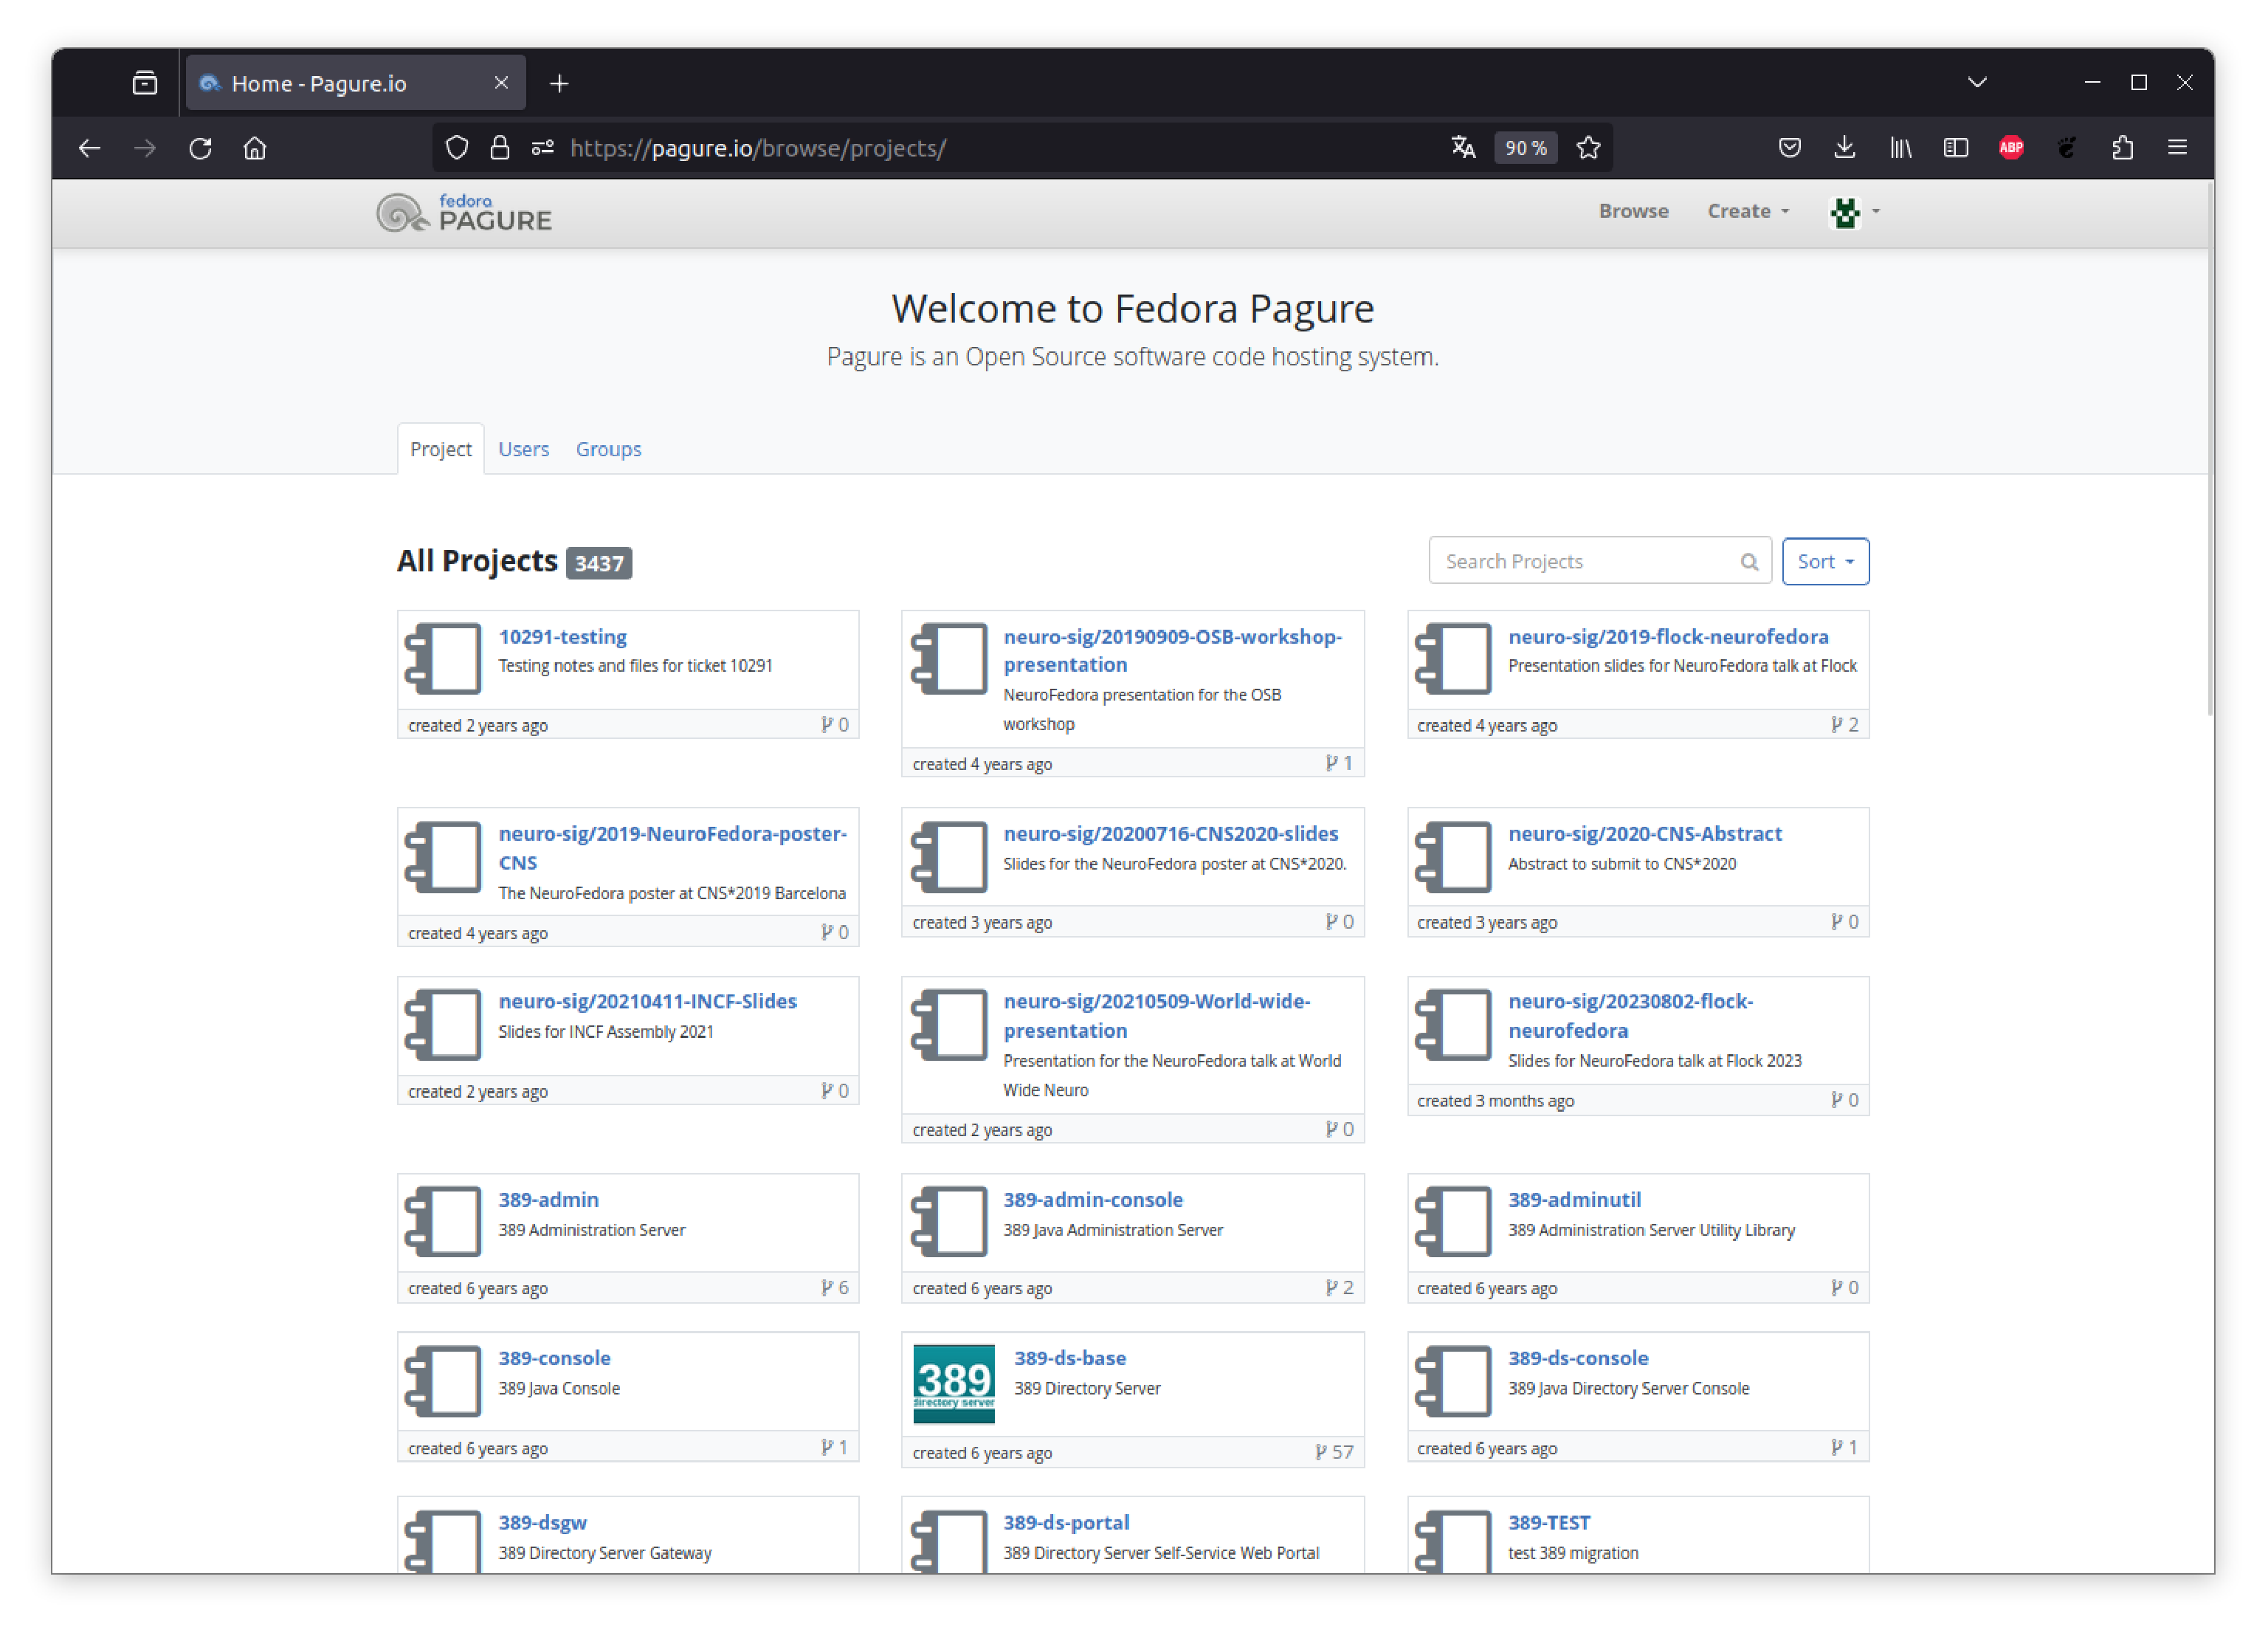
\includegraphics[width=0.75\textwidth,keepaspectratio=true,draft=\ddst]{img/rpms/pagure/pagure-0.eps}
\end{center}
\begin{enumerate}
\item On \href{https://pagure.io/}{Pagure} login using your Fedora Account credentials
\item Create a new ticket ACL: \href{https://pagure.io/settings/token/new}{https://pagure.io/settings/token/new}
\begin{center}
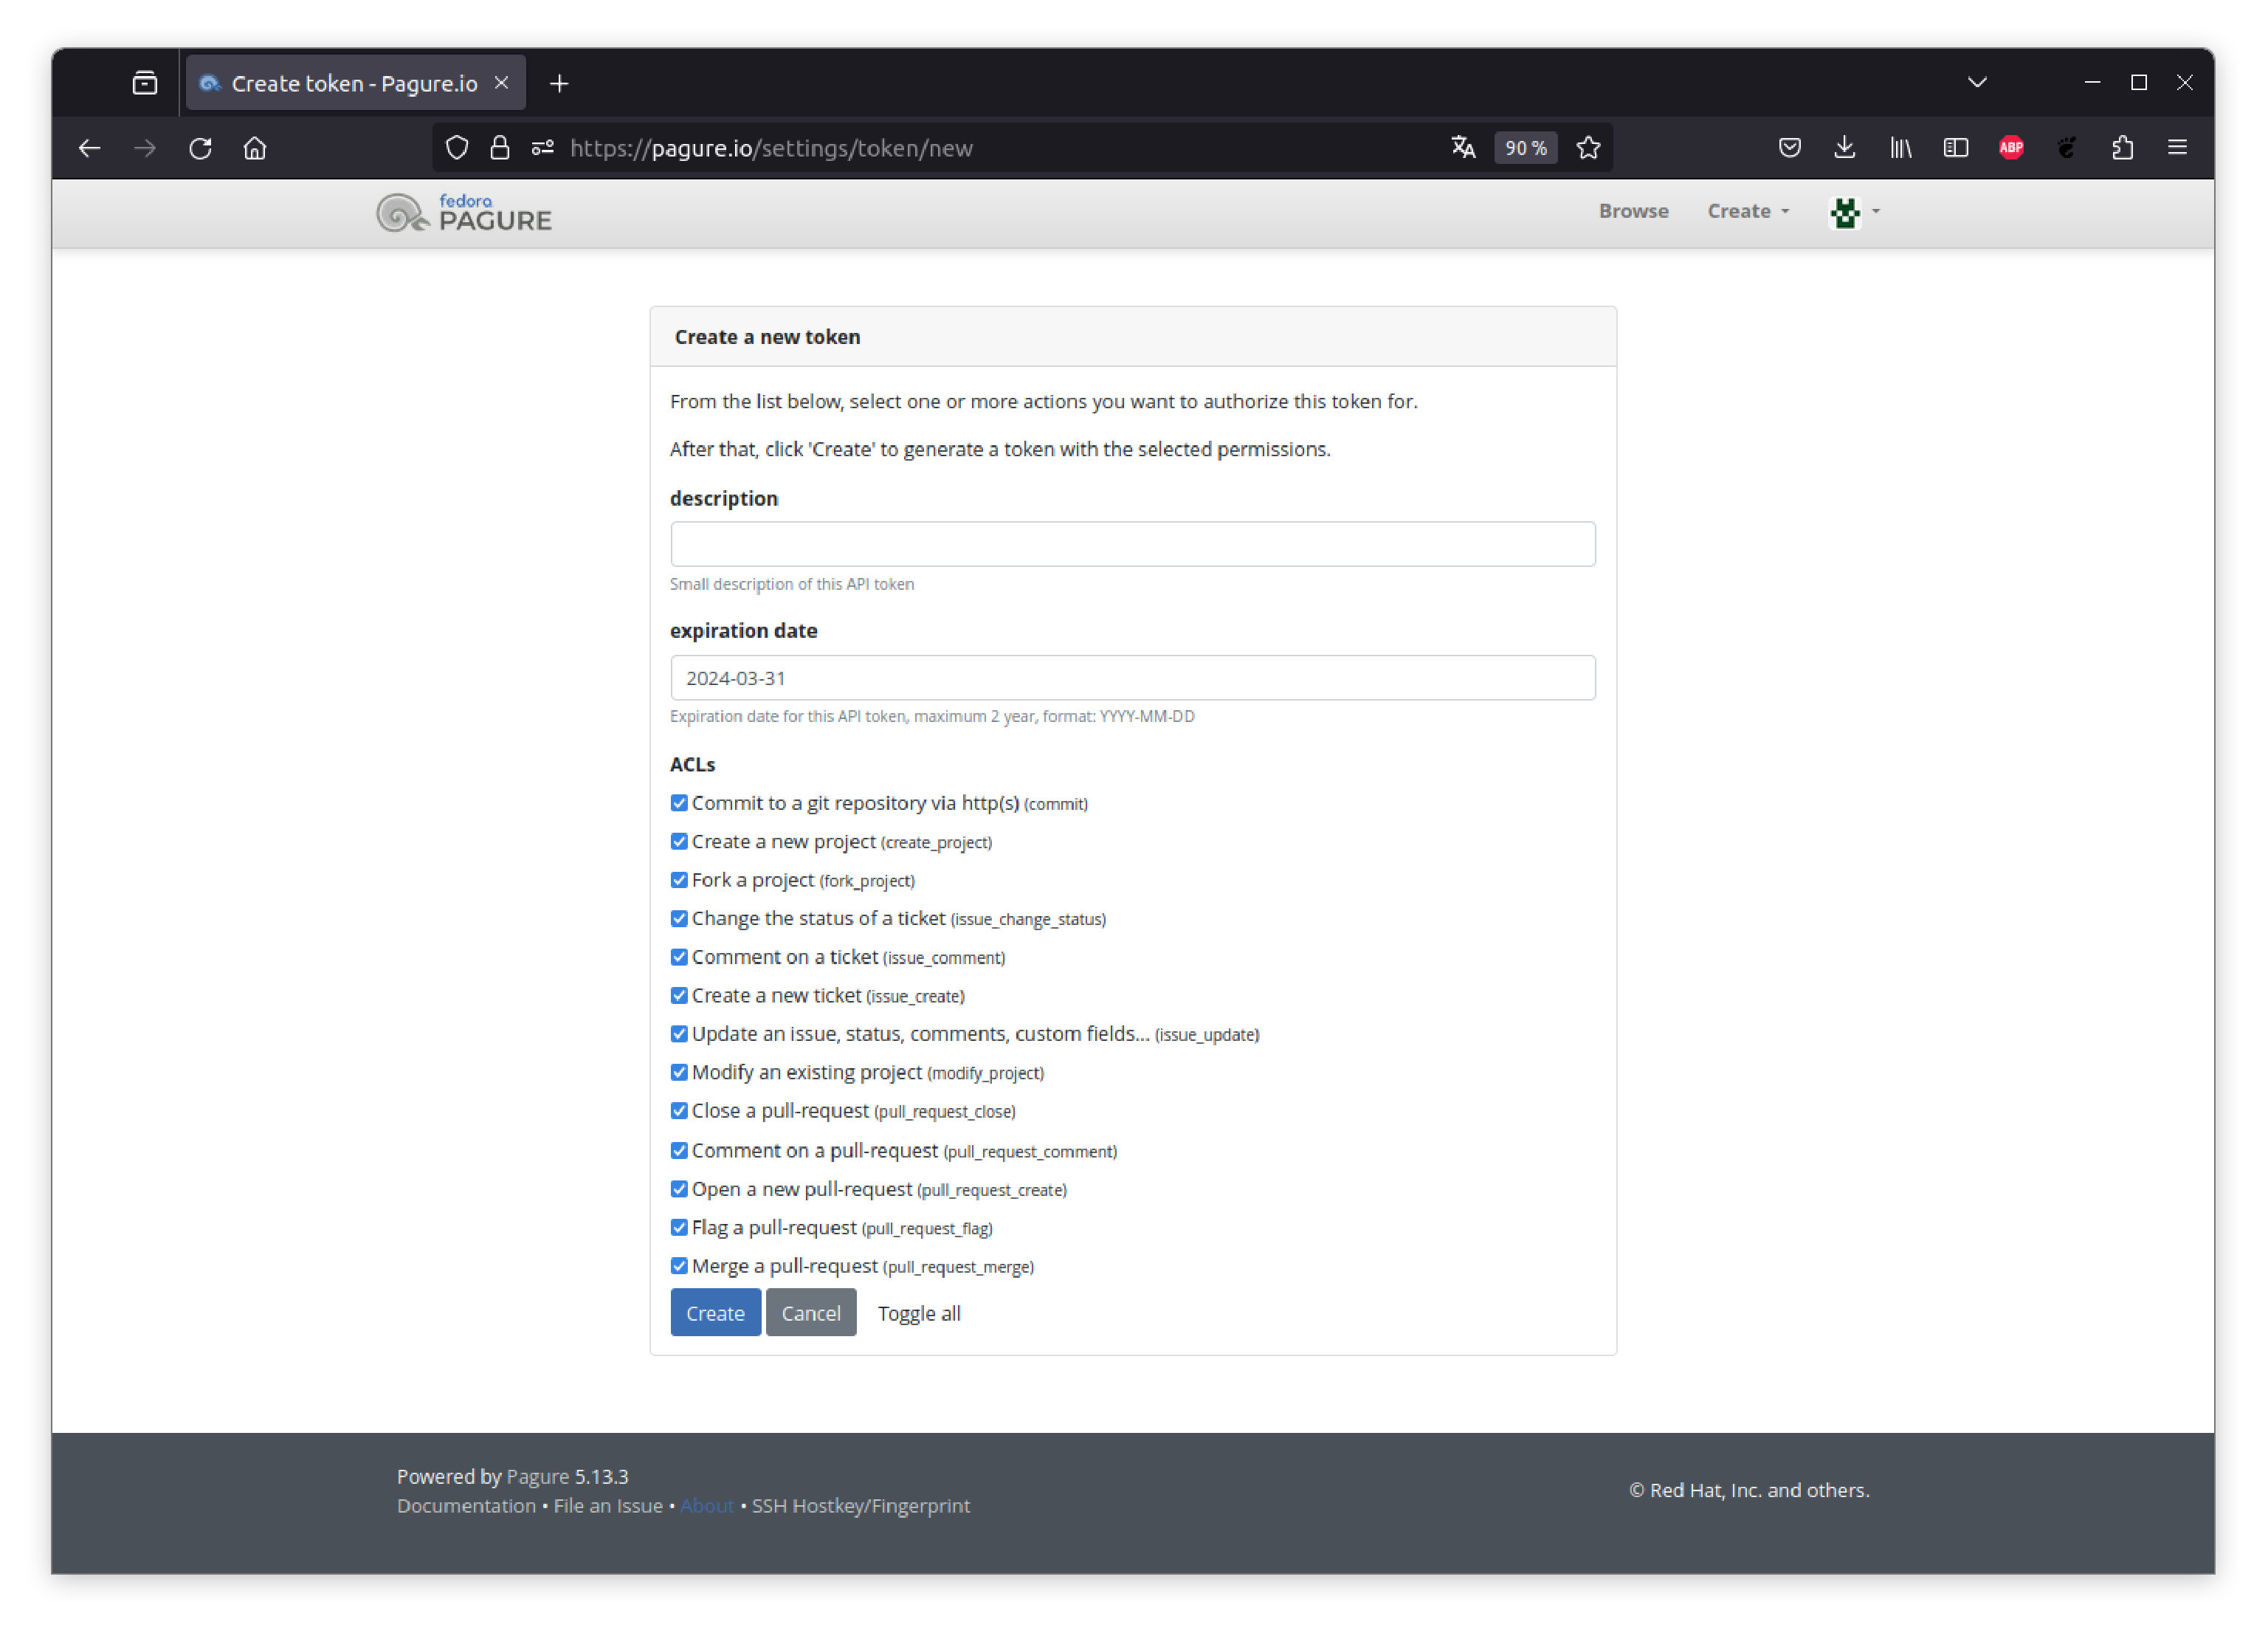
\includegraphics[width=0.75\textwidth,keepaspectratio=true,draft=\ddst]{img/rpms/pagure/pagure-1.eps}
\end{center}
You can select all available options, basically the system allows you create and work with set(s) of API Keys with different purposes. 
\item You can check the newly created API key in "\texttt{My Settings}" and then "\texttt{API Keys}"
\begin{center}
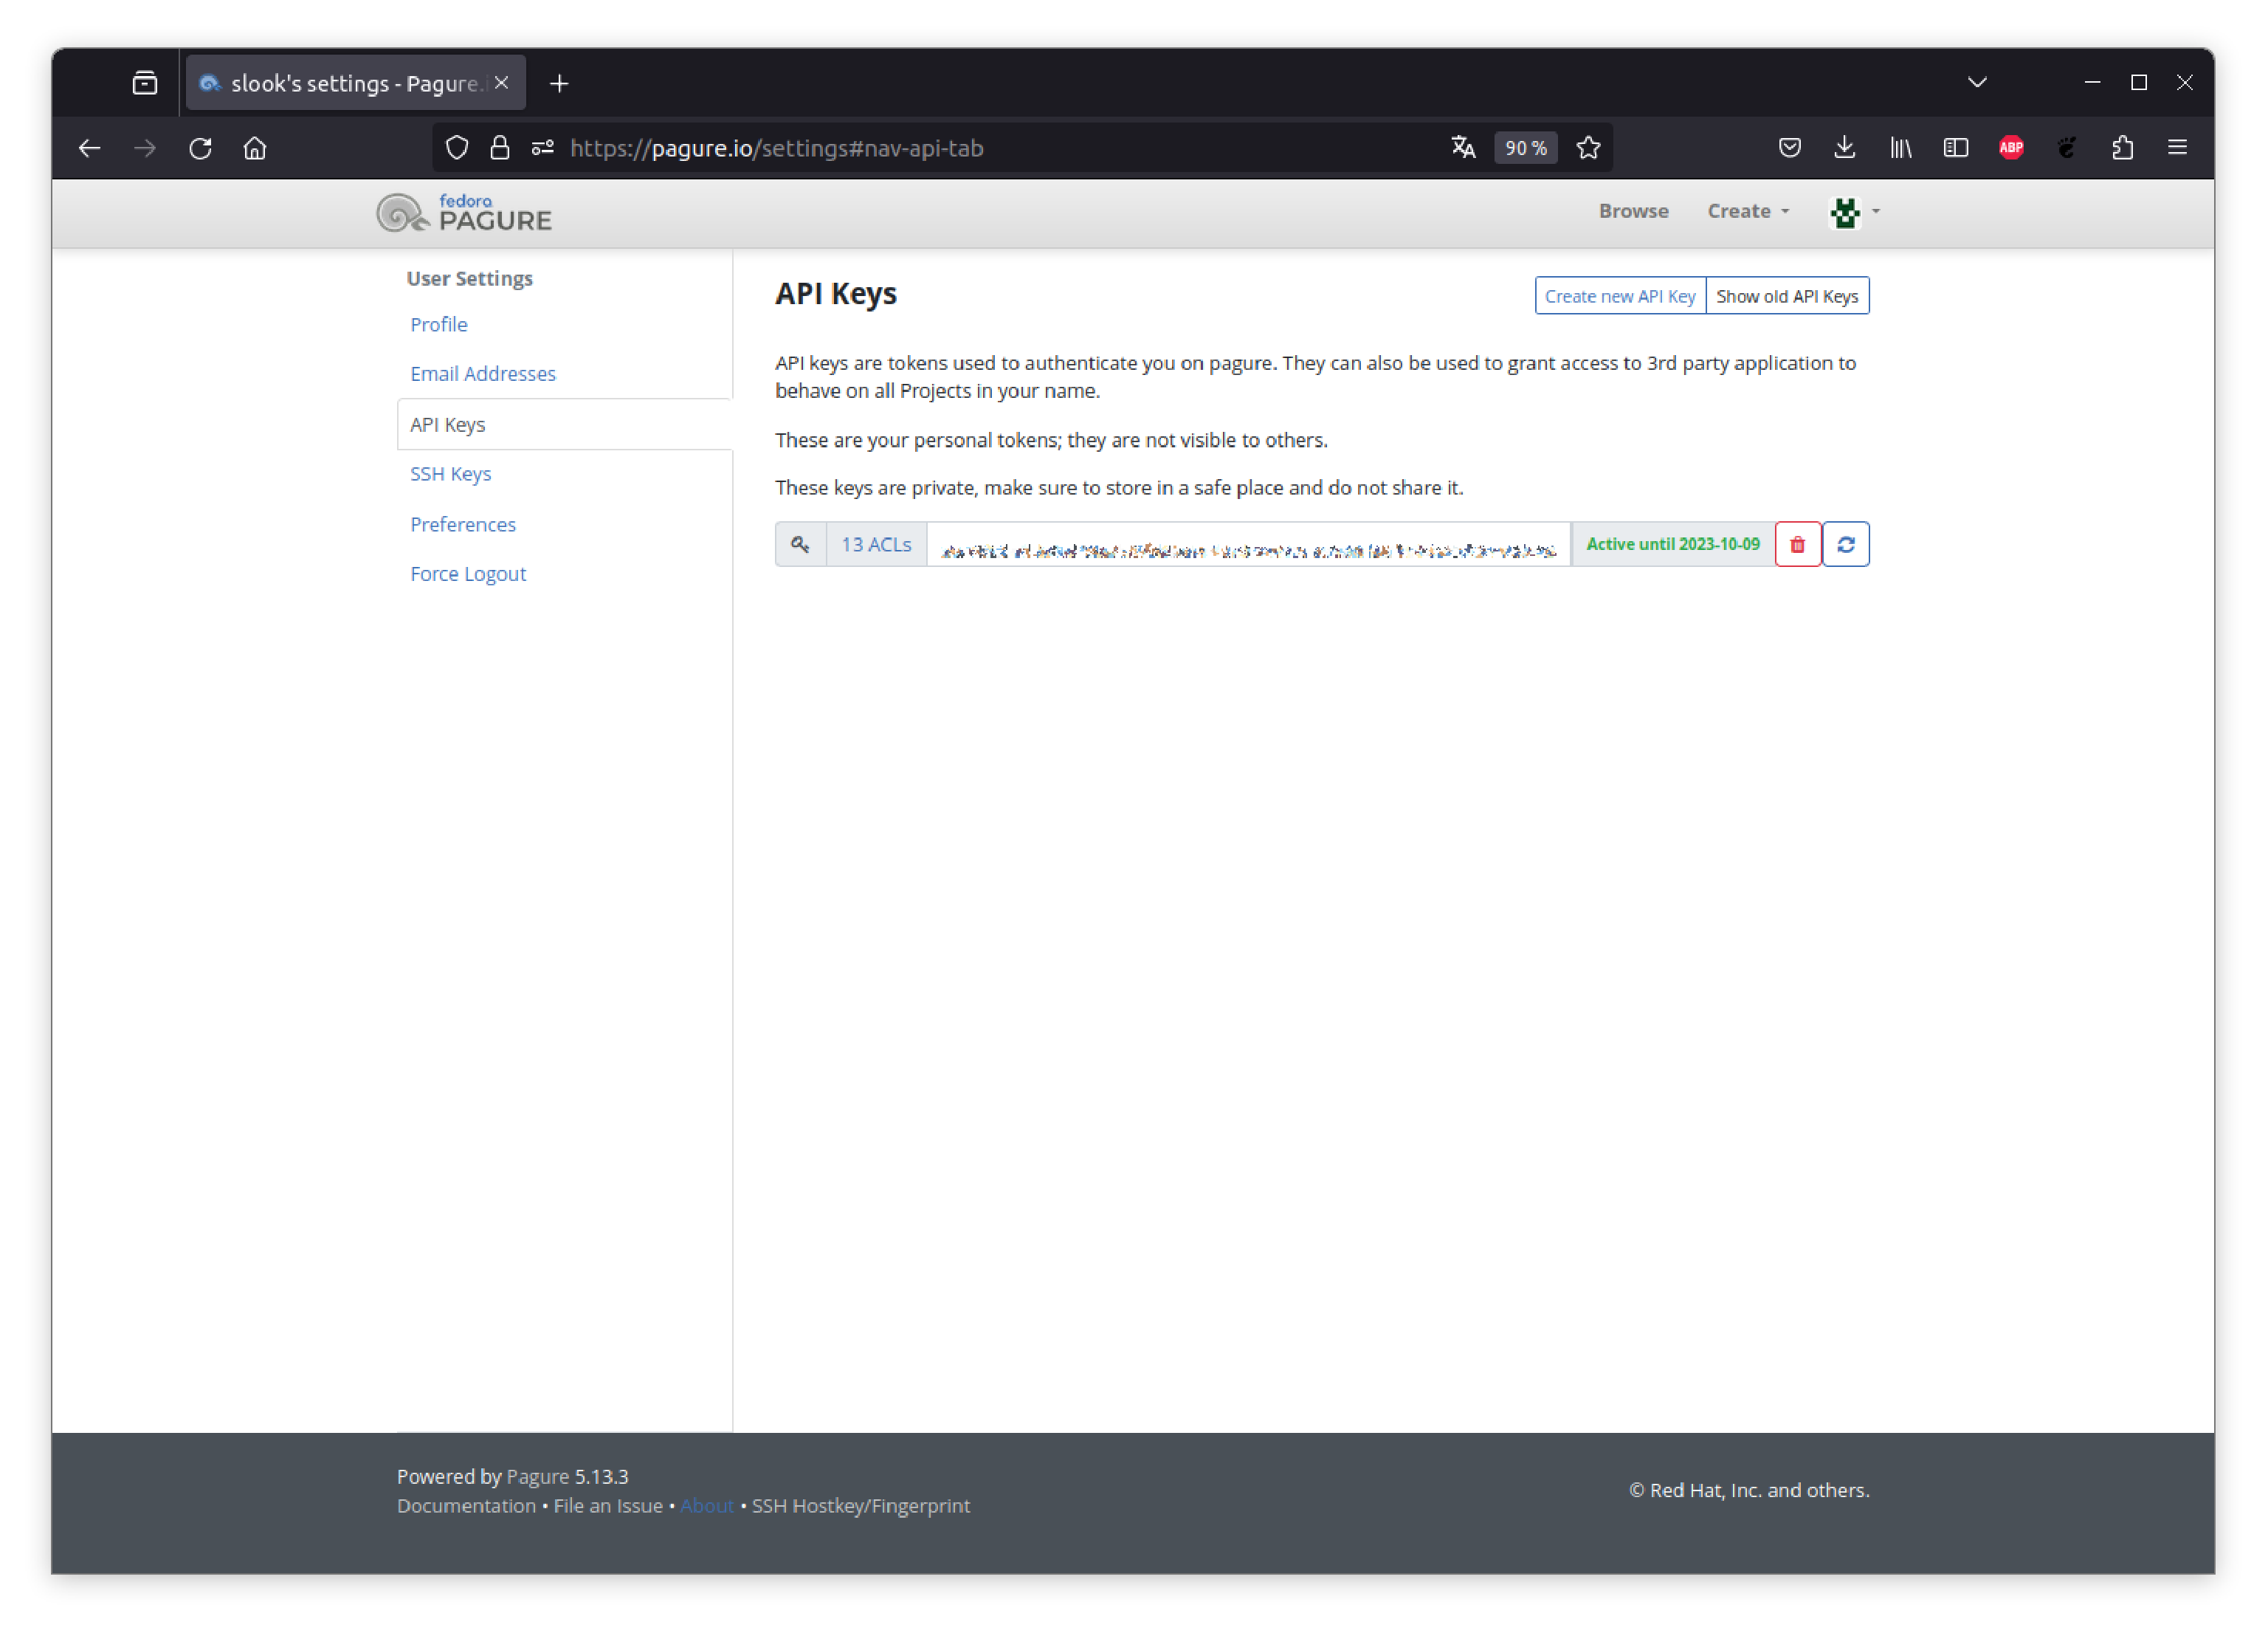
\includegraphics[width=0.75\textwidth,keepaspectratio=true,draft=\ddst]{img/rpms/pagure/pagure-3.eps}
\end{center}
\item Copy the content of the new key into: \texttt{\textasciitilde/.config/rpkg/fedpkg.conf}
\begin{scripti}
\fprompt{~} cat .config/rpkg/fedpkg.conf
[fedpkg.pagure]
url = https://pagure.io/
token = <generated-code-to-be-inserted-here>
\end{scripti}
\\[-0.75cm]
\noindent Note that the API key has an expiration date, so you will likely have to reproduce these few steps at some point in the future.
\end{enumerate}
This will ensure that the \bftt{fedpkg} command, a Fedora frontend to the \texttt{git} command, has the proper authorization access to handle the official repository of your package. 

\subsubsection{Creating the official repository for your package on \href{https://src.fedoraproject.org}{https://src.fedoraproject.org}}
\label{create_frepo}
Then it becomes possible to create the official source repository for your package. \\
The repository will be on the server \href{https://src.fedoraproject.org}{https://src.fedoraproject.org}, 
with the address:
\begin{center}https://src.fedoraproject.org/rpms/\texttt{program} \end{center}
This is where you will maintain you Fedora package, upload new source(s) and / or new package version(s). \\[0.25cm]
The repository creation is done using the \bftt{fedpkg} command:
\begin{script}
\fprompt{~} \bftt{fedpkg} \rtt{request-repo} program \dctt{???????}
\end{script}
Where: 
\begin{itemize}
\item \texttt{program} is the package name as provided in the bug message
\item \dctt{???????} is the bug message id number
\end{itemize}

\subsubsection{Uploading the package sources and / or "\texttt{.spec}" file to the official repository}

This is done using the \bftt{fedpkg} command, a Fedora frontend to the \texttt{git} command:
\begin{enumerate}
\item First, if not done already, configure your Git for Fedora packaging: 
{\small{
\begin{scripti}
\fprompt{~} \bftt{git} \rtt{config} \blue{--global} user.name "\abtt{Your Name}"
\fprompt{~} \bftt{git} \rtt{config} \blue{--global} user.email \dctt{\email}
\end{scripti}}}
\\[-0.75cm]
\item Then start by cloning the official source repository: 
\begin{scripti}
\fprompt{~} \bftt{fedpkg} \rtt{clone} prog
\end{scripti}
\\[-0.75cm]
\noindent This will copy the official Fedora source repository of "\texttt{program}" to your hard drive:
\begin{scripti}
\fprompt{~} ls prog
program.spec README.md sources
\fprompt{~}
\end{scripti}
\\[-0.75cm]
\noindent Note that you must use the name of the official Fedora repository as created in section~\ref{create_frepo}, in this case: "\texttt{program}"  
\item Download the sources from the official repository:  
\begin{scripti}
\fprompt{~} cd prog
\fprompt{~/program} \bftt{fedpkg} \rtt{sources}
\fprompt{~/program} ls
program.spec program-v1.1.tar.gz README.md sources
\fprompt{~/program}
\end{scripti}
\item Update the sources to the latest version:
\begin{scripti}
\fprompt{~/program} cp ~/program-v1.2.tar.gz .
\fprompt{~/program} \bftt{fedpkg} \rtt{new-sources} program-v1.2.tar.gz
\end{scripti}
\\[-0.75cm]
\noindent Before uploading new sources for your package to the official repository I strongly suggest that you already 
test-proofed the Koji build for this new package, see [Sec.~\ref{kojib}]. 
\item Modify the "\texttt{.spec}" file accordingly, including the \dgtt{\%changelog} section:
\begin{scripti}
\fprompt{~/program} vi program.spec 
\end{scripti}
\item Commit and push the changes:
\begin{scripti}
\fprompt{~/program} \bftt{fedpkg} \rtt{commit} \blue{-p -c}
\end{scripti}
\\[-0.75cm]
\noindent This will upload the new file(s) to: https://src.fedoraproject.org/rpms/\texttt{program}
\end{enumerate}

\subsubsection{Building the new package using the update(s)}

This is also done using the \bftt{fedpkg} command:
\begin{enumerate}
\item Request a build for Fedora branch(es), first of all for the rawhide branch:
{\small{
\begin{scripti}
\fprompt{~/program} \bftt{fedpkg} \rtt{request-branch} \blue{--repo} program \dgtt{rawhide}
\end{scripti}}}
\\[-0.5cm]
\noindent The rawhide branch is the development version of Fedora, usually the latest released version + 1. 
If the latest released is version 39 (f39), then rawhide will released as f40, 
then new rawhide branch will be created and later released as f41, and so on. \\[0.25cm]
To request a build for another Fedora branch, for instance the Fedora 39 branch, use:
{\small{
\begin{scripti}
\fprompt{~/program} \bftt{fedpkg} \rtt{request-branch} \blue{--repo} program \dgtt{f39}
\end{scripti}}}
\item To build the rawhide branch:
\begin{scripti}
\fprompt{~/program} \bftt{fedpkg} \rtt{switch-branch} \dgtt{rawhide}
\fprompt{~/program} \bftt{fedpkg} \rtt{build} \blue{--nowait}
\end{scripti}
To build the Fedora 39 branch: 
\begin{scripti}
\fprompt{~/program} \bftt{fedpkg} \rtt{switch-branch} \dgtt{f39}
\fprompt{~/program} \bftt{git} \rtt{merge} \blue{rawhide}:\dgtt{f39}
\fprompt{~/program} \bftt{git} \rtt{push} origin \blue{rawhide}:\dgtt{f39}
\fprompt{~/program} \bftt{fedpkg} \rtt{build} \blue{--nowait}
\end{scripti}
\\[-0.5cm]
\noindent For any other branch simply replace the \dgtt{f39} by the appropriate version number.
\end{enumerate}
At this stage you simply need to wait, the package will be built on Koji for the requested branches. 
If successful the builds will be available shortly to update the versions of the package in the Fedora software repository using the \href{https://bodhi.fedoraproject.org}{Bodhi} website.

\newpage
\subsubsection{Requesting for the new build(s) to update the package in the official repositories}

This is done via the web interface called Bodhi: \href{https://bodhi.fedoraproject.org}{https://bodhi.fedoraproject.org}. \\ 
\href{https://fedoraproject.org/wiki/Bodhi}{Bodhi} is a web-based system that facilitates the process of publishing package updates for Fedora. \\
\begin{center}
%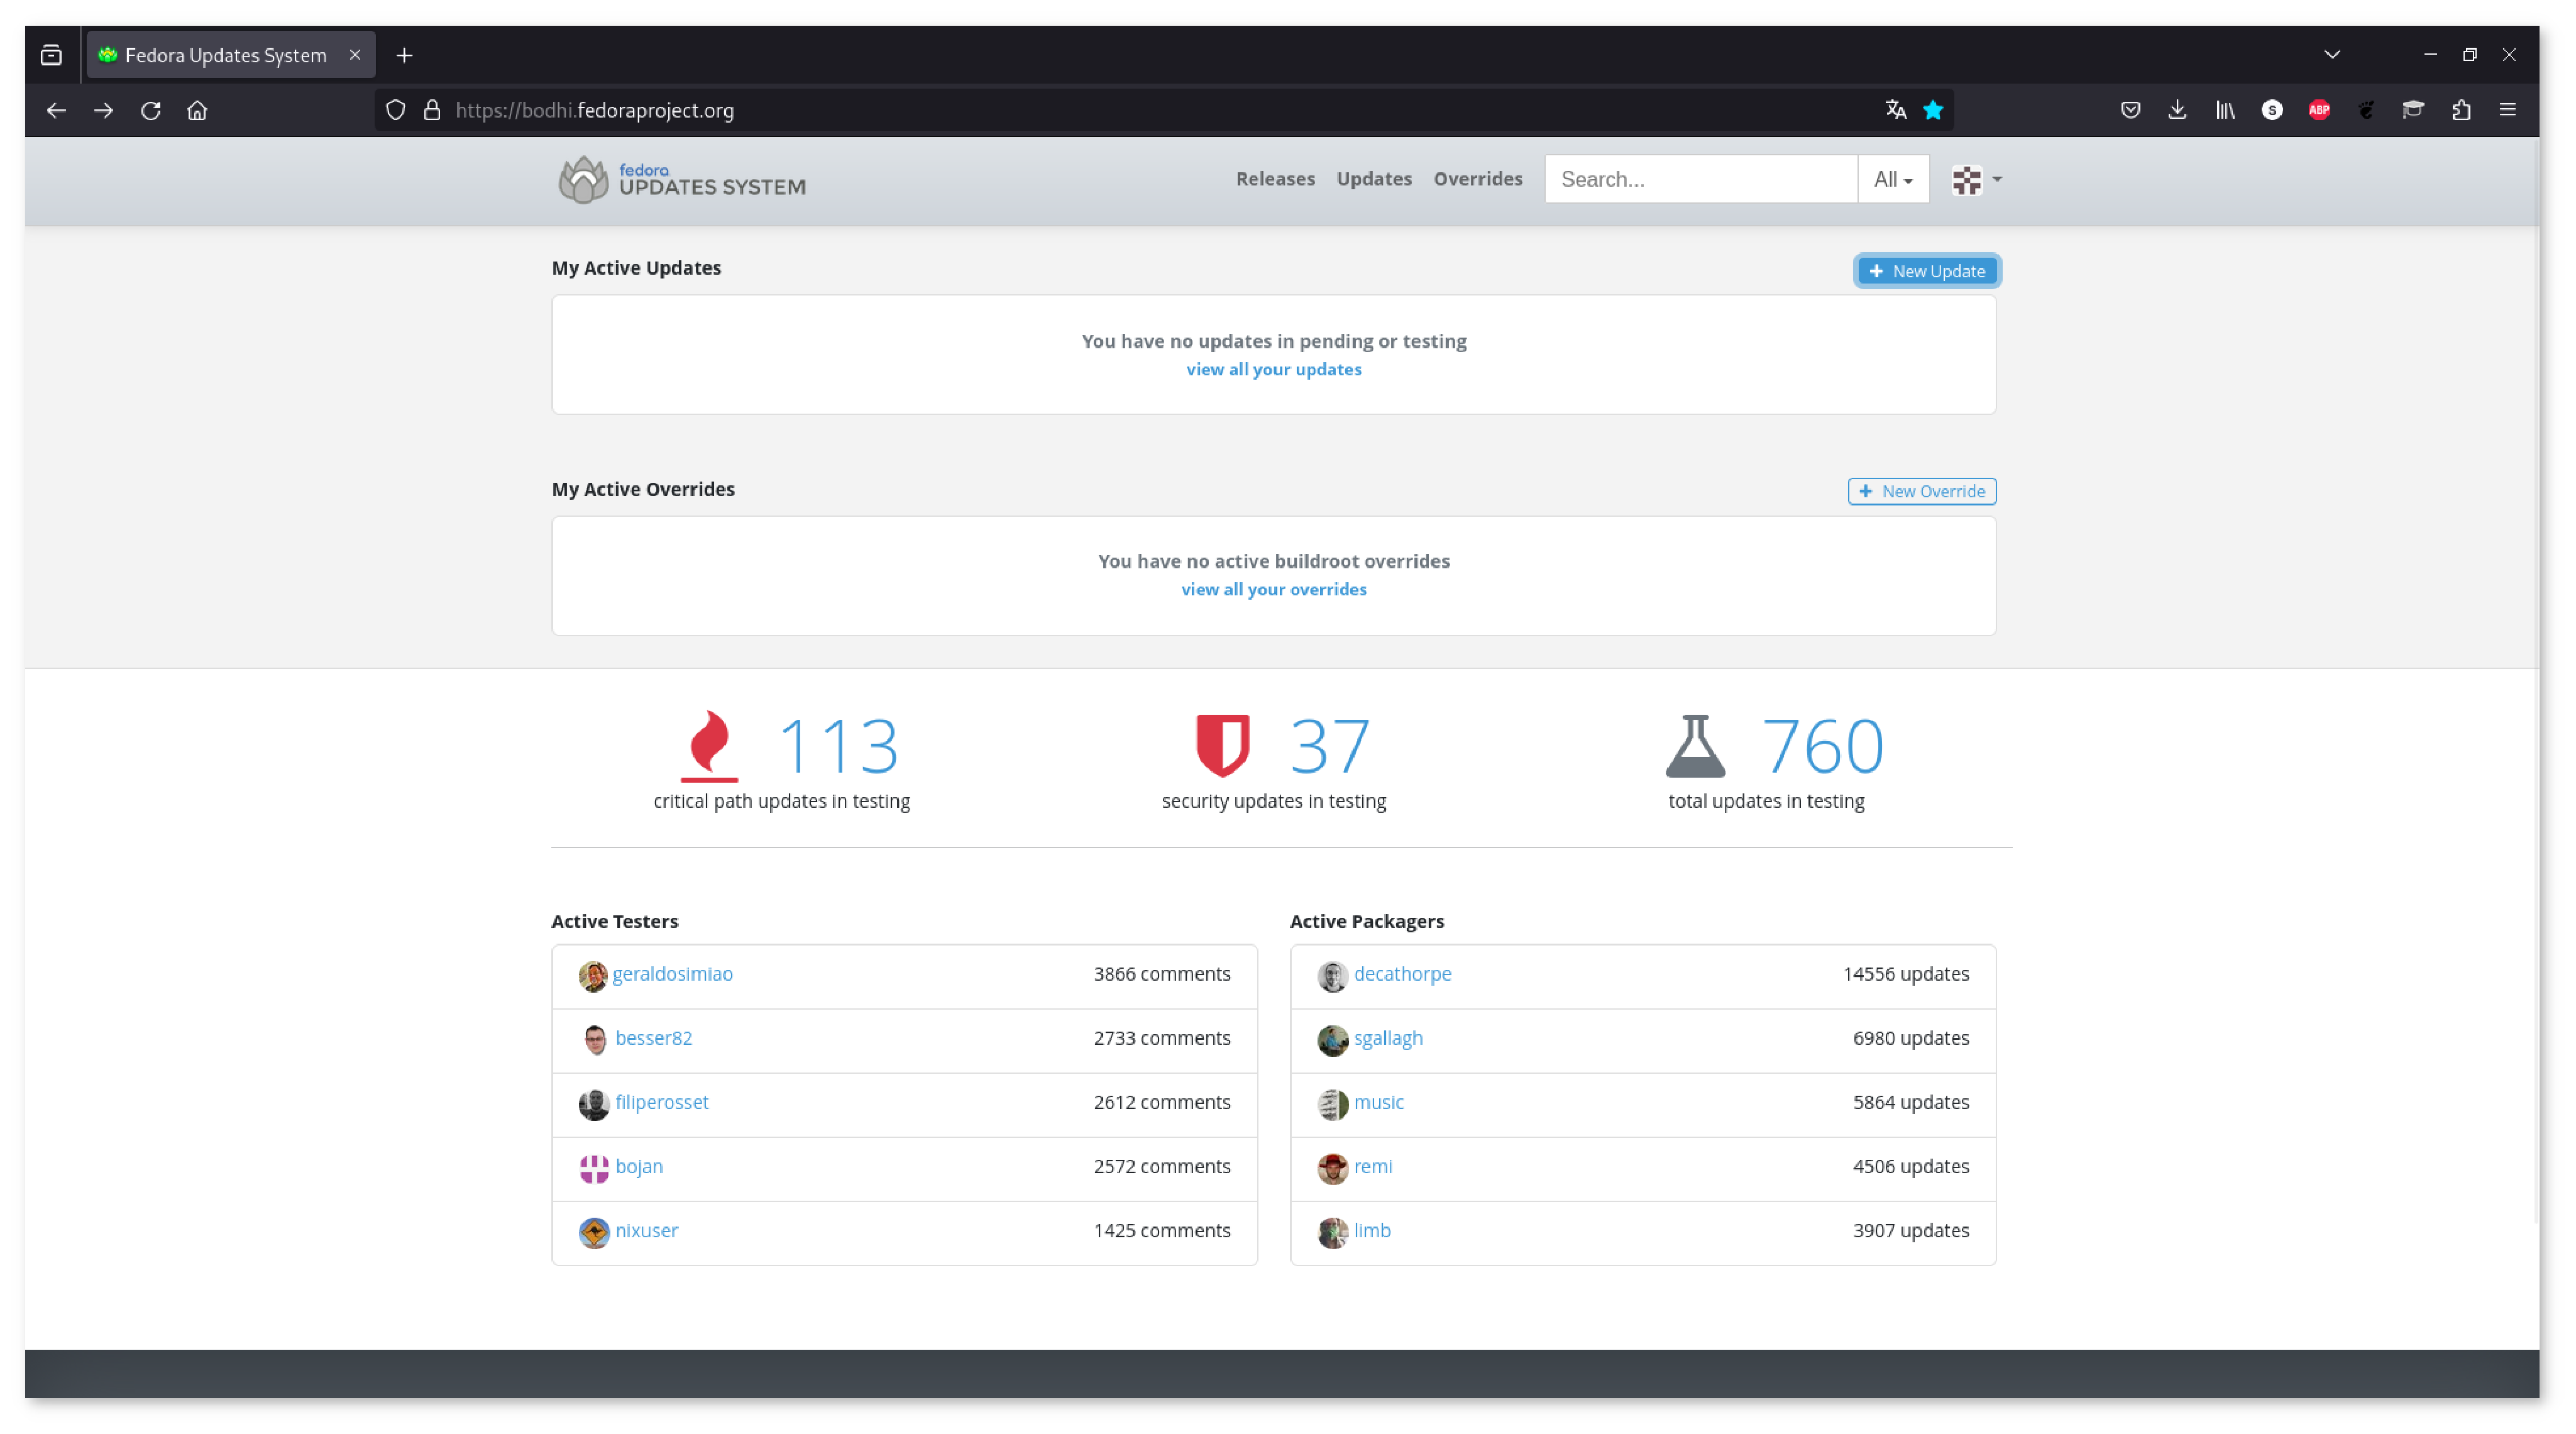
\includegraphics[width=0.75\textwidth,keepaspectratio=true,draft=\ddst]{img/rpms/bodhi/bodhi-0.eps}
\end{center}
To update the Fedora repositories with the new builds:
\begin{enumerate}
\item Login on Bodhi using your Fedora Account
\item Click on "\texttt{Updates}" 
\item Search for your package name, here "\texttt{program}" 
\item Need to create a new update to see what's next with more details
\end{enumerate}

\clearpage
